%––––––––––––––––––––––––––––––––––––––––––––––––––––––––––––––––––––––––––––––––––––––%
%––––––––––––––––––––––––––––––––––––––––––––––––––––––––––––––––––––––––––––––––––––––%
%–––––––––––––––––––––––––––––    S E T T I N G S        ––––––––––––––––––––––––––––––%
%––––––––––––––––––––––––––––––––––––––––––––––––––––––––––––––––––––––––––––––––––––––%
%––––––––––––––––––––––––––––––––––––––––––––––––––––––––––––––––––––––––––––––––––––––%
\sloppy



% Options for packages loaded elsewhere
\PassOptionsToPackage{hyphens}{url}
%
\documentclass[12pt, a4paper, ngerman, bidi=default]{article}

%––––––––––––––––––––––––––––––––––––––––––––––––––––––––––––––––––––––––––––––––––––––%
%–––––––––––––––––––––––––––––    S E T T I N G S     ––––––––––––––––––––––––––––––%
%–––––––––––––––––––––––––––––      P A K E T E        ––––––––––––––––––––––––––––––%
%–––––––––––––––––––––––––––––
%––––––––––––––––––––––––––––––––––––––––––––––––––––––––––––––––––––––––––––––––––––––%
\usepackage[utf8]{inputenc}
\usepackage[T1]{fontenc}
\usepackage[fixed]{fontawesome5} %Fontawesome für Icons und Symbole; siehe https://mirrors.ibiblio.org/CTAN/fonts/fontawesome5/doc/fontawesome5.pdf
\usepackage{amsmath,amssymb}
\usepackage{tcolorbox}
\usepackage{afterpage}
\usepackage{multicol}
\usepackage{graphicx}
\usepackage{subcaption} %Für die Verwendung von subfigure
\usepackage{setspace} %Für den Befehl \setstretch
\usepackage{transparent}
\usepackage{tikz}
  \usetikzlibrary{shapes.geometric, arrows.meta,fit, backgrounds, calc, positioning}
\usepackage{pgf-pie}%Für Kreisdiagramme
\usepackage{pgfplots}%Für Diagramme
  \pgfplotsset{compat=1.18}
\usepackage{eso-pic}%Für Hintergrundbilder
\usepackage{fvextra}    %Muss vor csquotes geladen werden
% \usepackage{csvsimple}%Für CSV-Dateien
% \usepackage{booktabs}   %für \toprule, \midrule, \bottomrule
% \usepackage{longtable}  %falls nicht schon geladen
% \usepackage{placeins}%Für \FloatBarrier
\usepackage[autostyle, german=quotes]{csquotes}
\usepackage[
  backend=biber,
  style=authoryear-ibid,
  autocite=footnote,  % Automatisch Fussnote
  language=ngerman,
  citetracker,
  ibidtracker,
  shorthandibid=true,
  backref=true,
  backrefstyle=three+
]{biblatex}
\let\cite\footcite


\DeclareBibliographyAlias{software}{misc}
\DefineBibliographyStrings{ngerman}{%
  page = {S\adddot},
  pages = {S\adddot\addspace ff\adddot}
}
\DefineBibliographyStrings{ngerman}{
  urlseen = {Zugriff am}
}
\DeclareFieldFormat{urldate}{\addspace#1}

\renewbibmacro*{url+urldate}{%
  \printfield{url}%
  \setunit*{\addspace}%
  \iffieldundef{urldate}
    {}
    {\printtext[urldate]{\printurldate}}%
}

\setlength{\skip\footins}{20pt}
\addbibresource{/Users/svenburkhardt/Developer/masterarbeit/1_MA_Arbeit/assets/Literature_Bib/Exportierte Einträge.bib}

\renewbibmacro*{date}{% 
    \ifentrytype{online}{% Falls der Eintrag @online ist, nimm das urldate
        \printtext[parens]{Zugriff am \usebibmacro{urldate}}}{\printdate}
    
}

\usepackage[ngerman]{babel}
\usepackage{pifont} %Für die Kästchen und Häkchen-Symbole
\usepackage[dvipsnames,svgnames,x11names,table]{xcolor}
\usepackage[table]{xcolor}
%Zum Definieren und Verwenden von Farben
\definecolor{LightGray}{gray}{0.9}
\definecolor{MediumGray}{gray}{0.7}
\definecolor{UniRot}{HTML}{D20537}                  %Corperate Design Farben Uni Basel 
\definecolor{UniAnthrazit}{HTML}{46505A}            %Corperate Design Farben Uni Basel 
\definecolor{UniMint}{HTML}{A5D7D2}                 %Corperate Design Farben Uni Basel 
\definecolor{VeryLightGray}{gray}{0.95}%Sehr helles Grau
\definecolor{OldPaper}{HTML}{f4eade}


\definecolor{UniBlue}{HTML}{1F78B4}     %Kräftiges Blau
\definecolor{UniGold}{HTML}{FFB000}     %Goldgelb
\definecolor{UniViolet}{HTML}{6A3D9A}   %Violett

\definecolor{abbrev}{RGB}{255,153,153}             %Rot für Tags
\definecolor{add}{RGB}{204,255,238}                %Hellgrün/Türkis für Tags
\definecolor{sic}{RGB}{255,255,153}                %Hellgelb für Tags
\definecolor{unclear}{RGB}{255,230,184}            %Hellorange für Tags
\definecolor{date}{RGB}{153,153,255}               %Blau für Tags
\definecolor{organization}{RGB}{255,153,255}       %Pink für Tags
\definecolor{place}{RGB}{204,153,255}              %Lila für Tags
\definecolor{person}{RGB}{153,255,153}             %Hellgrün für Tags
\definecolor{signature}{RGB}{153,255,153}          %Hellgrün (gleiche Farbe wie Person) für Tags
\definecolor{eventTag}{HTML}{05A9FF}               %Blau für Tags
\definecolor{oldLetter}{RGB}{246,238,227}          %Beige für Hintergrund  
\definecolor{vscode-blue}{HTML}{569CD6}            %VSCode Blau für python
\definecolor{vscode-yellow}{HTML}{DCDCAA}          %VSCode Gelb für python
\newcommand{\code}[1]{\colorbox{VeryLightGray}{\texttt{#1}}} %für die darstellung von Code 

\usepackage{array}
\usepackage{minted}
\usepackage{capt-of}
\usepackage{wrapfig}
\usepackage{colortbl}
\usepackage{booktabs}
\usepackage[hyphens]{url}
\usepackage{ragged2e}
\usepackage[
  hidelinks,
  unicode=true,
  hyperfootnotes=true,
  colorlinks=true,
  linkcolor=Blue,
  filecolor=Maroon,
  citecolor=Blue,
  urlcolor=Blue,
  pdfborder={0 0 0}
]{hyperref}
\usepackage{nameref}
\newcommand{\parref}[1]{Abschnitt \nameref{#1}}
\usepackage{orcidlink}
\usepackage{iftex}
\ifPDFTeX%
  \usepackage[utf8]{inputenc}
  \usepackage{lmodern}
  % Authblk, pdfpages etc. hier einbinden
\else
  \usepackage{fontspec}
\fi


% Use upquote if available, for straight quotes in verbatim environments
\IfFileExists{upquote.sty}{\usepackage{upquote}}{}

% Paragraph spacing configuration depending on the class
\makeatletter
\@ifundefined{KOMAClassName}{% if non-KOMA class
  \IfFileExists{parskip.sty}{%
    \usepackage{parskip}
 }{% else
    \setlength{\parindent}{0pt}
    \setlength{\parskip}{0pt}}
}{% if KOMA class
  \KOMAoptions{parskip=half}}
\makeatother


\usepackage[lmargin=2.5cm,rmargin=2.5cm,tmargin=2cm,bmargin=2cm]{geometry}
\setlength{\emergencystretch}{3em}%prevent overfull lines
\setcounter{secnumdepth}{-\maxdimen}%remove section numbering
% Make \paragraph and \subparagraph free-standing
\makeatletter
\ifx\paragraph\undefined\else
  \let\oldparagraph\paragraph%
  \renewcommand{\paragraph}{
    \@ifstar%
      \xxxParagraphStar%
      \xxxParagraphNoStar%
 }
  \newcommand{\xxxParagraphStar}[1]{\oldparagraph*{#1}\mbox{}}
  \newcommand{\xxxParagraphNoStar}[1]{\oldparagraph{#1}\mbox{}}
\fi
\ifx\subparagraph\undefined\else
  \let\oldsubparagraph\subparagraph%
  \renewcommand{\subparagraph}{
    \@ifstar%
      \xxxSubParagraphStar%
      \xxxSubParagraphNoStar%
 }
  \newcommand{\xxxSubParagraphStar}[1]{\oldsubparagraph*{#1}\mbox{}}
  \newcommand{\xxxSubParagraphNoStar}[1]{\oldsubparagraph{#1}\mbox{}}
\fi
\makeatother


\providecommand{\tightlist}{%
  \setlength{\itemsep}{0pt}\setlength{\parskip}{0pt}}\usepackage{longtable,booktabs,array}
\usepackage{calc}%for calculating minipage widths
% Correct order of tables after \paragraph or \subparagraph
\usepackage{etoolbox}
\makeatletter
\patchcmd\longtable{\par}{\if@noskipsec\mbox{}\fi\par}{}{}
\makeatother
% Allow footnotes in longtable head/foot
\IfFileExists{footnotehyper.sty}{\usepackage{footnotehyper}}{\usepackage{footnote}}
\makesavenoteenv{longtable}
\makeatletter
\def\maxwidth{\ifdim\Gin@nat@width>\linewidth\linewidth\else\Gin@nat@width\fi}
\def\maxheight{\ifdim\Gin@nat@height>\textheight\textheight\else\Gin@nat@height\fi}
\makeatother
% Scale images if necessary, so that they will not overflow the page
% margins by default, and it is still possible to overwrite the defaults
% using explicit options in \includegraphics[width, height, ...]{}
\setkeys{Gin}{width=\maxwidth,height=\maxheight,keepaspectratio}
% Set default figure placement to htbp
\makeatletter
\def\fps@figure{htbp}
\makeatother
% definitions for citeproc citations
\NewDocumentCommand\citeproctext{}{}
\NewDocumentCommand\citeproc{mm}{%
  \begingroup\def\citeproctext{#2}\cite{#1}\endgroup}
\makeatletter
%allow citations to break across lines
 \let\@cite@ofmt\@firstofone%
%avoid brackets around text for\cite:
 \def\@biblabel#1{}
 \def\@cite#1#2{{#1\if@tempswa, #2\fi}}
\makeatother
\newlength{\cslhangindent}
\setlength{\cslhangindent}{1.5em}
\newlength{\csllabelwidth}
\setlength{\csllabelwidth}{3em}
\newenvironment{CSLReferences}[2]%#1 hanging-indent, #2 entry-spacing
 {\begin{list}{}{%
  \setlength{\itemindent}{0pt}
  \setlength{\leftmargin}{0pt}
  \setlength{\parsep}{0pt}
 %turn on hanging indent if param 1 is 1
  \ifodd #1 \else%chktex 1
   \setlength{\leftmargin}{\cslhangindent}
   \setlength{\itemindent}{-1\cslhangindent}
  \fi
 %set entry spacing
  \setlength{\itemsep}{#2\baselineskip}}}
 {\end{list}}
\usepackage{calc}
\newcommand{\CSLBlock}[1]{\hfill\break\parbox[t]{\linewidth}{\strut\ignorespaces#1\strut}}
\newcommand{\CSLLeftMargin}[1]{\parbox[t]{\csllabelwidth}{\strut#1\strut}}
\newcommand{\CSLRightInline}[1]{\parbox[t]{\linewidth-\csllabelwidth}{\strut#1\strut}} %chktex 8
\newcommand{\CSLIndent}[1]{\hspace{\cslhangindent}#1}

\makeatletter
\@ifpackageloaded{caption}{}{\usepackage{caption}}
\AtBeginDocument{%
\ifdefined\contentsname%
  \renewcommand*\contentsname{Inhaltsverzeichnis}
\else
  \newcommand\contentsname{Inhaltsverzeichnis}
\fi
\ifdefined\listfigurename%
  \renewcommand*\listfigurename{Abbildungsverzeichnis}
\else
  \newcommand\listfigurename{Abbildungsverzeichnis}
\fi
\ifdefined\listtablename%
  \renewcommand*\listtablename{Tabellenverzeichnis}
\else
  \newcommand\listtablename{Tabellenverzeichnis}
\fi
\ifdefined\figurename%
  \renewcommand*\figurename{Abbildung}
\else
  \newcommand\figurename{Abbildung}
\fi
\ifdefined\tablename%
  \renewcommand*\tablename{Tabelle}
\else
  \newcommand\tablename{Tabelle}
\fi
}
\@ifpackageloaded{float}{}{\usepackage{float}}
\floatstyle{ruled}
\@ifundefined{c@chapter}{\newfloat{codelisting}{h}{lop}}{\newfloat{codelisting}{h}{lop}[chapter]}
\floatname{codelisting}{Listing}
\providecommand{\listoflistings}{\listof{codelisting}{Listingverzeichnis}}
\makeatother
\makeatletter
\makeatother
\makeatletter
\@ifpackageloaded{caption}{}{\usepackage{caption}}
\@ifpackageloaded{subcaption}{}{\usepackage{subcaption}}
\makeatother

% get rid of language-specific shorthands (see #6817):
\let\LanguageShortHands\languageshorthands%
\def\languageshorthands#1{}
\usepackage{bookmark}

\usepackage{placeins}                  %für \FloatBarrier
\usepackage[toc,page]{appendix}        %für eigene Anhangs-Umgebung
% optional:
% \usepackage{pdfcrypt}                  %für PDF-Passwortschutz

\IfFileExists{xurl.sty}{\usepackage{xurl}}{}%add URL line breaks if available
\urlstyle{same}%disable monospaced font for URLs
\hypersetup{
  pdftitle={Konzeption für AG Masterarbeit am
17.01.2025},
  pdfauthor={Sven Burkhardt},
  pdflang={de},
  colorlinks=true,
  linkcolor={blue},
  filecolor={Maroon},
  citecolor={Blue},
  urlcolor={Blue},
  pdfcreator={LaTeX via pandoc}
}

\usepackage{etoolbox}
\makeatletter
\providecommand{\subtitle}[1]{% add subtitle to \maketitle
  \apptocmd{\@title}{\par {\large #1 \par}}{}{}
}
\makeatother
\title{\vspace*{4cm} \LARGE Digitale Harmonie aus historischer Dissonanz
\color{UniMint} \rule{8cm}{1pt} \\  
\vspace{0.2cm}  
\color{white}\large Extraktion, Ordnung und Analyse\\unstrukturierter Archivdaten\\des Männerchor Murg}
\usepackage{etoolbox}
\makeatletter
\providecommand{\subtitle}[1]{% add subtitle to \maketitle
  \apptocmd{\@title}{\par {\large #1 \par}}{}{}
}
\makeatother
\subtitle{}
\author{Sven Burkhardt}
\date{2025-08-14}%chktex 8

%––––––––––––––––––––––––––––––––––––––––––––––––––––––––––––––––––––––––––––––––––––––%
%––––––––––––––––––––––––––––––––––––––––––––––––––––––––––––––––––––––––––––––––––––––%
%––––––––––––––––––––––––––––– T I T E L B L A T T   ––––––––––––––––––––––––––––––––––%
%––––––––––––––––––––––––––––––––––––––––––––––––––––––––––––––––––––––––––––––––––––––%
%––––––––––––––––––––––––––––––––––––––––––––––––––––––––––––––––––––––––––––––––––––––%
\begin{document}
\begin{titlepage}
    
% Setzt die Schriftfarbe auf Weiss
\color{white}
\pagecolor[HTML]{46505A} %Seitenfarbe in Uni Basel Anthrazit D20537 (rot)
\pagenumbering{gobble}   %Verhindert die Anzeige der Seitennummer auf dem Titelblatt
\date{}
\author{}
\maketitle
\begin{center}
  \author{\LARGE{\author{\vspace{-0.5cm}Sven Burkhardt}}}\\
  \vspace{4mm}
  \large{\orcidlink{0009-0001-4954-4426} {0009-0001-4954-4426}}\\%chktex 8%Orcid Link und Nummer
  \begin{figure}[h]
    \centering
    \color{white}
    \large{\href{https://dhlab.philhist.unibas.ch/en/persons/sven-burkhardt/}{{\hspace*{0.5mm}
\includegraphics[height=4.5
  mm]{./assets/Logos/Uni_basel_logo_white.png}}\hspace{3.4mm}\color{white} 17-056-912}}\\%chktex 8 %logo Unibas + Link + Immatrikulationsnummer
    \faIcon[regular]{calendar-alt}\date{\hspace*{2mm}15.08.2025}% chktex 8
  \end{figure}
  \setcounter{figure}{0}
\end{center}


% ------------ Hexagon grafik beginn -----------
\centering
\AddToShipoutPictureBG*{%
    \put(0,-40){%
        
\includegraphics[width=\paperwidth]{./assets/Logos/Hexagon_Deko}
  }
}
\centering
\AddToShipoutPictureBG*{%
    \put(0,810){%
        
\includegraphics[width=\paperwidth]{./assets/Logos/Hexagon_Deko}
   }
}
\centering
\AddToShipoutPictureBG*{%
    \put(33,752){%
        
\includegraphics[width=\paperwidth]{./assets/Logos/Hexagon_Deko}
   }
}
\centering
\AddToShipoutPictureBG*{%
    \put(-99,752){%
        
\includegraphics[width=\paperwidth]{./assets/Logos/Hexagon_Deko}
   }
}



\noindent%Verhindert Einzug des nachfolgenden Textes
% ------------ Hexagon grafik ende -----------



\begin{center}
    \vfill
    \begin{figure}
        \centering
        \begin{subfigure}{.3\textwidth}
          \centering
          
\includegraphics[width=.8\linewidth]{./assets/Logos/uni-basel-logo-en_white.png}
        \end{subfigure}%
        \begin{subfigure}{.3\textwidth}
          \centering
          
\includegraphics[width=.8\linewidth]{./assets/Logos/dhlab-logo-white.png}
        \end{subfigure}
    \end{figure}
        \setcounter{figure}{0}

    University of Basel\\
    Digital Humanities Lab\\
    Switzerland
\end{center}


\newpage
\color{black}          %Setzt die Schriftfarbe auf Schwarz für die folgenden Seiten
\setstretch{1.5}
\end{titlepage}
\newpage
%________________

%________________

%––––––––––––––––––––––––––––––––––––––––––––––––––––––––––––––––––––––––––––––––––––––%
%––––––––––––––––––––––––––––––––––––––––––––––––––––––––––––––––––––––––––––––––––––––%
%–––––––––––––––––––––––––––––   A B S T R A C T     ––––––––––––––––––––––––––––––––––%
%––––––––––––––––––––––––––––––––––––––––––––––––––––––––––––––––––––––––––––––––––––––%
%––––––––––––––––––––––––––––––––––––––––––––––––––––––––––––––––––––––––––––––––––––––%


\pagecolor{white}  
\color{black}  %Textfarbe zurücksetzen
\color{black} 
\setstretch{1.5}


\newpage 
Diese Arbeit befasst sich mit dem Archiv des Männerchor Murg in den Jahren des Zweiten Weltkrieges. 
Hierfür wird eine automatisierte Pipline auf Basis von LLMs und Patternmatching vorgestellt, mit deren Hilfe Named Entities extrahiert und weiterverarbeitet werden. 
Ziel ist es, dieses Archiv digital zugänglich, die beteiligten Personen sowie deren Netzwerke und dessen geographische Ausdehnung sichtbar zu machen.



%––––––––––––––––––––––––––––––––––––––––––––––––––––––––––––––––––––––––––––––––––––––%
%–––––––––––––––––––––––––––––      T A B L E        ––––––––––––––––––––––––––––––––––%
%–––––––––––––––––––––––––––––        O F            ––––––––––––––––––––––––––––––––––%
%–––––––––––––––––––––––––––––   C O N T E N T S     ––––––––––––––––––––––––––––––––––%
%––––––––––––––––––––––––––––––––––––––––––––––––––––––––––––––––––––––––––––––––––––––%



\newpage
\renewcommand*\contentsname{Inhaltsverzeichnis}%This controls the title of your table of contents.
{
\hypersetup{linkcolor=}
\setcounter{tocdepth}{5}%Sets the maximum sublevel to be displayed within the table of contents.
\tableofcontents
}
\pagenumbering{arabic}\setstretch{1.5}%Overwrites the previous command, pages are counted as normal from this point.


%––––––––––––––––––––––––––––––––––––––––––––––––––––––––––––––––––––––––––––––––––––––%
%––––––––––––––––––––––––––––––––––––––––––––––––––––––––––––––––––––––––––––––––––––––%
%––––––––––––––––––––––––      I N T R O D U C T I O N    ––––––––––––––––––––––%
%––––––––––––––––––––––––––––––––––––––––––––––––––––––––––––––––––––––––––––––––––––––%
%––––––––––––––––––––––––––––––––––––––––––––––––––––––––––––––––––––––––––––––––––––––%
\newpage
\section{Einleitung}
\subsection{Ziel und Relevanz der Arbeit}
\subsection{Formulierung der Forschungsfrage}
\subsection{Aufbau der Arbeit}
\subsection{Geografischer und historischer Kontext}
Die vorliegende Arbeit stützt sich auf Unterlagen aus dem Archiv des \enquote{Männerchor Murg} dessen Nachfolge im Jahr 2021 
durch die \enquote{New Gospelsingers Murg} angetreten wurde. Murg ist eine deutsche Gemeinde am Hochrhein, 
rund 30 km Luftlinie von Basel entfernt. Der Ort liegt am gleichnamigen Fluss Murg, der in den Rhein mündet. 
Beide Gewässer bildeten über Jahrhunderte hinweg den wirtschaftlichen Motor der Region: Die Wasserkraft der Murg 
begünstigte früh die Ansiedlung von Mühlen, Hammerwerken und Schmieden entlang des Bachlaufs, während der Rhein mit seiner 
Drahtseil-Fähre eine bedeutende Verkehrs- und Handelsverbindung bot, die bis zum Ersten Weltkrieg privat betrieben wurde.

Mit dem Ausbau der Landstrasse, der heutigen Bundesstrasse 34, sowie dem Anschluss an die Bahnstrecke Basel–Konstanz 
entwickelte sich Murg im 19. Jahrhundert von einer landwirtschaftlich geprägten Siedlung zu einer Gewerbe-, Handels- und 
Industriegemeinde. Die Wasserkraft wurde dabei zu einem entscheidenden Standortfaktor: Die Ansiedlung der Schweizer 
Textilfirma \textit{Hüssy \& Künzli AG} im Jahr 1853\cite[vgl.][]{gemeinde_murg_geschichte_nodate} trug wesentlich 
zum wirtschaftlichen Wachstum der Gemeinde bei. Zahlreiche Arbeitskräfte, vor allem aus der benachbarten Schweiz, 
machten Murg zu einem wichtigen Standort der regionalen Textilindustrie.

Die Gründung des \textit{Männerchor Murg} im Jahr 1861 durch Schweizer Textilarbeiter belegt diesen engen Zusammenhang 
zwischen wirtschaftlicher Migration, Industrialisierung und lokalem Vereinswesen. Diese historische Verflechtung bildet 
eine zentrale Grundlage für die vorliegende Untersuchung.


  

\newpage
\section{Forschungsstand und Forschungslücke}\label{subsec:forschungsstand}

Die vorliegende Arbeit knüpft an zwei Vorarbeiten an, die in den Jahren 2018 und 2022 am Departement Geschichte der Universität Basel durchgeführt
werden. In zwei Transkribus-Seminaren werden erste Teilbestände der \enquote{Männerchor Akten 1925--1944} erschlossen und in einem Korpus
von 137 Einzeldokumenten zusammengeführt.\cite[vgl.][]{burkhardt_feldpost_2022}
Ein kleinerer Korpus von rund 50 Dokumenten wird mit Metadaten versehen. Erfasst werden unter anderem die genaue Position im Ordner auf Seitenebene, 
Kurztitel und Entstehungsdatum. Diese Metadaten bilden die Grundlage für eine erstmalige systematische Erschliessung.

Während in einem frühen Projektschritt vorrangig häufig genannte Personennamen (\enquote{Carl Burger}, \enquote{Fritz Jung})
dokumentiert werden, richtet sich der Fokus im zweiten Schritt auf die Feldpost. Ziel ist es, über die Auswertung der Feldpostnummern
Rückschlüsse auf beteiligte Militäreinheiten, deren Stationierungen und Verlagerungen während des Zweiten Weltkriegs zu ziehen.

Für diese Recherchen kommen einschlägige Fachliteratur zu den jeweiligen Fachgebieten zum Einsatz. 
Hier sind besonders die Bücher von Alex Buchner\cite[vgl.][]{buchner_handbuch_1989}, Christian Hartmann\cite[vgl.][]{hartmann_wehrmacht_2010}, 
Werner Haupt\cite[vgl.][]{haupt_buch_1982}, Christoph Rass\cite[vgl.][]{rass_deutsche_2009}, Georg Tessin\cite[vgl.][]{tessin_verbande_1977} 
und Christian Zentner\cite[vgl.][]{zentner_illustrierte_1983} zu nennen.

Darüberhinaus werden eigene Recherchen in den Beständen des \textit{Bundesarchivs – Militärarchiv Freiburg}\cite{hollmann_freiburg_2025} durchgeführt. Ergänzende Recherchen 
stammen aus den Suchlisten des \textit{Deutschen Roten Kreuzes (DRK)}\cite{reuter_drk_2025}. Hinzu kommen philatelistische Übersichts-Websites\cite{noauthor_feldpost_nodate}, 
die bei der Entzifferung von Briefmarken und Stempeln helfen.
Absoult essentiell für den Erfolg dieser Recherchen sind Citizen-Science-Foren\footnote{vor Allem werden verwendet: 
\textit{Forum der Wehrmacht}~\parencite{hermans_forum_nodate} und das \textit{Lexikon der Wehrmacht}~\parencite{altenburger_lexikon_nodate}.}. Sie ergänzen und validieren eigene Forschung.

Parallel zur inhaltlichen Erschliessungen entsteht 2022 eine erste digitale Storymap mit \textit{ArcGIS},
die zentrale Ergebnisse des Projekts öffentlich zugänglich macht. Grundlage bildet die Sichtung, konservatorische Aufbereitung und Digitalisierung
von zunächst rund 30 der etwa 800 Seiten Vereinsakten. Der Teilkorpus wird entheftet, gescannt und mit Metadaten wie Absender, Datum,
Feldpostnummer und Einheit versehen. Da jedes Dokument einen anderen Verfasser aufweist, erfolgt die Transkription manuell. Eine automatische Handschriftenerkennung 
ist aufgrund der heterogenen Schriftbilder nicht praktikabel.
Am Beispiel einzelner Sänger wie \textit{Emil Durst} lässt sich durch die Rechercheergebnisse mithilfe der Feldpostnummern und ergänzender Kartenmaterialien der Aufenthaltsort
bis auf Gebäude oder wenige Meter genau rekonstruieren. Diese Erkenntnisse werden mit historischen Karten, Luftbildern und Ortsrecherchen verknüpft
und in einer interaktiven ArcGIS-Karte visualisiert, die Stationierungen, Märsche und Frontverschiebungen der Chormitglieder anschaulich darstellt. 

Die in diesen Vorprojekten erarbeiteten Listen, Geodaten, Transkriptionen und Visualisierungen fliessen in die vorliegende Arbeit ein
und bilden eine wesentliche Grundlage für die erweiterte, automatisierte Pipeline, die im Folgenden vorgestellt wird. Dazu gehören beispielsweise auch die Verbandsabzeichen, 
Taktische Zeichen\cite[vgl][S.64-66]{haupt_buch_1982} der jeweiligen Einheiten, die auch in die Groundtruth der vorliegenden Arbeit inkorporiert werden.

Abgesehen von diesen Vorarbeiten ist der Quellenkorpus wissenschaftlich unerschlossen. Mit dieser Arbeit liegt erstmals eine
umfassendere wissenschaftliche Auswertung vor.

Mit der notwendigen manuellen Recherche in oben dargelegten Datenbankstrukturen wird zugleich sichtbar, wie sehr es an Brücken fehlt, 
um unterschiedliche Klassifikationen, fachspezifische Ordnungslogiken und semantische Webtechnologien nachhaltig miteinander zu verbinden. Ein verhältnismässig einfaches
Webscraping nach Informationen zu diesem Korpus ist nahezu unmöglich. Ausgeführt werden diese Probleme beispielsweise bei 
Smiraglia und Scharnhorst (2021)\cite[vgl.][]{richard_linking_2022}, 
 die anhand konkreter Fallstudien verdeutlichen, wie fragmentiert semantische Strukturen bislang entwickelt werden 
 und welche Hürden bei der praktischen Verknüpfung heterogener Wissensorganisationen bestehen. Dabei benennen sie insbesondere die 
 Herausforderungen bei der Übersetzung historisch gewachsener Klassifikationen in standardisierte semantische Formate, 
 die Notwendigkeit dauerhafter technischer Wartung und die Abhängigkeit von nachhaltigen Infrastruktur-Partnern\cite[vgl.][Kap. 2 und 5]{richard_linking_2022}.

Für eine Einordnung zu historischen Netzwerkanaylsen sei auf Gamper\&Reschke\cite{gamper_knoten_2015} verwiesen. Der Sammelband
\textit{Knoten und Kanten III} verdeutlicht, dass die historische Netzwerkanalyse zwar von einem interdisziplinär etablierten Methodenkanon 
profitiert, jedoch nach wie vor vor erheblichen Herausforderungen steht. Dazu zählen die Fragmentierung historischer Quellen, der hohe manuelle 
Erfassungsaufwand und methodische Desiderate im Umgang mit zeitlichen und räumlichen Dimensionen. Erschwerende Faktoren einer systematische Erfassung 
relationaler Strukturen. Dennoch eröffnen netzwerkanalytische Verfahren – besonders im Zusammenspiel mit relationaler Soziologie 
und Figurationsansätzen – neue Perspektiven auf Macht, Abhängigkeiten und Akteurskonstellationen in historischen Gesellschaften.






%––––––––––––––––––––––––––––––––––––––––––––––––––––––––––––––––––––––––––––––––––––––%
%––––––––––––––––––––––––––––––––––––––––––––––––––––––––––––––––––––––––––––––––––––––%
%––––––––––––––––––––––––              Korpus            ––––––––––––––––––––––%
%––––––––––––––––––––––––––––––––––––––––––––––––––––––––––––––––––––––––––––––––––––––%
%––––––––––––––––––––––––––––––––––––––––––––––––––––––––––––––––––––––––––––––––––––––% 
\section{Korpus}\label{section:Korpus}
Aus dem Bestand des Ordners \textit{``Männerchor Akten 1925--1944''} werden für diese Arbeit ausschliesslich Akten verwendet, 
die während des Zweiten Weltkriegs verfasst wurden. Der Analysezeitraum erstreckt sich dementsprchend zwischen dem 01. September 1939 
und dem 8. Mai 1945, dem Tag der bedingungslosen Kapitulation Deutschlands.

Die zeitliche Eingrenzung ist notwendig, um die Funktionalität der im Folgenden beschriebenen Pipeline 
in einem klar definierten historischen Kontext demonstrieren zu können. Gleichzeitig führt TeXshop?diese Auswahl zu einer 
bewussten Reduzierung der potenziell erfassten Akteurinnen und Akteure, Orte und Organisationen. Diese Fokussierung ist 
insbesondere im Hinblick auf die Erstellung einer verlässlichen Groundtruth bedeutsam, die durch ergänzende Archivrecherchen 
mit historischen Metadaten angereichert wird.

Die Kombination aus einer präzise definierten Quellengrundlage und der digitalen Anreicherung dient dazu, das 
Potenzial der computergestützten Auswertung historischer Dokumente exemplarisch aufzuzeigen. 
Zugleich unterstreicht sie, dass die Qualität der Ergebnisse wesentlich von der sorgfältigen Eingrenzung 
des Korpus und der manuellen Validierung und Anreicherung abhängt.
%––––––––––––––––––––––––––––––––––––––––––––––––––––––––––––––––––––––––––––––––––––––%
%––––––––––––––––––––––––              Quellen            ––––––––––––––––––––––%
%––––––––––––––––––––––––––––––––––––––––––––––––––––––––––––––––––––––––––––––––––––––%

\subsection{Quellen}
\subsubsection{Quellentradierung}
In den Lagerräumen der New Gospel Singers Murg, dem Nachfolgeverein des Männerchors Murg, 
wird im Jahr 2018 mehrere je ca. 800 Seiten umfassende Ordner mit historischen Unterlagen gefunden. 
Für diese Arbeit wird ein Ordner mit der Aufschrift \textit{\enquote{Männerchor Akten 1925--1944}} gewählt, da er neben dem Ordner 
\textit{\enquote{Männerchor Akten 1946--1950}} den grössten Zeitraum abdeckt. Darüberhinaus bietet er das Potential, 
aufschlussreiche Einblicke in das Vereinsleben in der Zeit vor und während des Nationalsozialismus, insbesondere des Zweiten Weltkrieges, zu geben.\\ 
Der Ordner umfasst insgesamt 780 Seiten und deren Inhalt kann als \enquote{Protokoll}, \enquote{Brief}, \enquote{Postkarte}, \enquote{Rechnung}, 
\enquote{Regierungsdokument}, \enquote{Noten}, \enquote{Zeitungsartikel}, \enquote{Liste}, \enquote{Notizzettel} oder \enquote{Offerte} kategorisiert werden.

Die Unterlagen könnten bereits direkt nach ihrer Entstehung in die Ordner eingelegt worden sein. Einzelne Akten sind mit einem 
\enquote{Heftstreifen}, auch \enqute{Aktendulli} genannt, zusammengefehtet. In der Plastikversion, wie er in diesen Akten vorliegt, wurde er bereits 1938 patentiert\cite[vgl.][]{noauthor_heftstreifen_2023}.
Wer die Akten so archiviert hat lässt sich nicht mehr sagen. 
Der sogenannte \enquote{Archival-Bias} des Archivars, also die Grundeinstellung, weshalb etwas aufbewahrt oder
vernichtet wurde, lässt sich damit nicht mehr feststellen. 

\subsubsection{Quellenbeschrieb}\label{Dokumententypen}
\noindent
\begin{minipage}[t]{0.49\textwidth}
  \setstretch{1.5}
  \justifying
  Für diese Arbeit wurde ein Korpus selektiert, dessen Auswahl in~\nameref{section:Korpus} näher beschrieben wird. 
  Erfasst, benannt und tabellarisch mit groben Metadaten versehen werden sämtliche Unterlagen aus dem Ordner \textit{\enquote{Männerchor Akten 1925--1944}}. 
  Diese Auflistung in der Datei \textit{Akten\_Gesamtübersicht.csv} erlaubt die Zuordnung zu folgenden Kategorien: Briefe, Postkarten, Protokolle, Regierungsdokumente, Zeitungsartikel, 
  Rechnungen und Offerten. Die Verteilung ist ungleichmässig: Briefe bilden mit 282 von 381 Seiten die grösste Kategorie; Rechnungen und Offerten sind jeweils nur einseitig vertreten.
\end{minipage}%
\hfill
\begin{minipage}[t]{0.49\textwidth}
  \centering
  \vspace*{0.3cm} % Feinjustierung nach Bedarf
  \begin{tikzpicture}
    \begin{axis}[
      ybar,
      bar width=16pt,
      height=5.5cm,
      ymin=0,
      ylabel={Anzahl Dokumente},
      symbolic x coords={Brief, Postkarte, Protokoll, Regierungsdok., Zeitungsartikel, Rechnung, Offerte},
      xtick=data,
      nodes near coords,
      nodes near coords align={vertical},
      x tick label style={rotate=45, anchor=east},
      axis lines=left,
      enlarge x limits=0.15,
      grid=major,
      grid style={dashed, gray!30},
    ]
      \addplot[fill=gray!60] coordinates {
        (Brief,282) 
        (Postkarte,51) 
        (Protokoll,36) 
        (Regierungsdok.,5) 
        (Zeitungsartikel,4) 
        (Rechnung,1) 
        (Offerte,1)
      };
    \end{axis}
  \end{tikzpicture}

  \captionof{figure}{Verteilung der Dokumententypen im untersuchten Bestand (150 Akten – 381 Seiten).}
  \label{fig:dokumententypen-bar}
\end{minipage}

\noindent
\begin{minipage}[t]{0.48\textwidth}
  \setstretch{1.5}
  \justifying
  Auf Grundlage der oben erwähnten, händisch erstellten Gesamtliste der Akten können durch 
  die systematische Benennung der Dokumente auch Rückschlüsse auf den bislang nicht untersuchten 
  Teil des Bestandes gezogen werden. Mithilfe des Sprachmodells von OpenAI wurde eine grobe Näherung zur 
  Zusammensetzung des restlichen Korpus erarbeitet, wie sie in der rechtsstehenden Darstellung visualisiert ist.
  
  Diese Übersicht erhebt keinen Anspruch auf Vollständigkeit oder Genauigkeit, sondern dient der Veranschaulichung, 

\end{minipage}%
\hfill
\begin{minipage}[t]{0.48\textwidth}
  \centering
  \vspace*{0.2cm} % Feinjustierung der vertikalen Ausrichtung
  
  \begin{tikzpicture}
    \begin{axis}[
      ybar,
      bar width=16pt,
      height=5.5cm,
      ymin=0,
      ylabel={geschätzte Verteilung restlicher Korpus},
      symbolic x coords={Briefe, Postkarten, Protokolle, Regierungsdok., Zeitungsartikel, Rechnungen, Offerten},
      xtick=data,
      nodes near coords,
      nodes near coords align={vertical},
      x tick label style={rotate=45, anchor=east},
      axis lines=left,
      enlarge x limits=0.15,
      grid=major,
      grid style={dashed, gray!30},
    ]
      \addplot[fill=gray!60] coordinates {
        (Briefe,155) 
        (Postkarten,12) 
        (Protokolle,7) 
        (Regierungsdok.,60) 
        (Zeitungsartikel,25) 
        (Rechnungen,8) 
        (Offerten,12)
      };
    \end{axis}
  \end{tikzpicture}
  \captionof{figure}{geschätzte Verteilung der Dokumententypen im restlichen Bestand.}\label{fig:dokumententypen-schätzung}
\end{minipage}

\vspace{1em}

\noindent
dass die Verteilung der Quellengattungen im Zeitraum vor dem Zweiten Weltkrieg möglicherweise deutlich anders gestaltet ist. Eine vertiefte Untersuchung dieser bislang unbearbeiteten Bestände erscheint daher notwendig und markiert eine zentrale Forschungslücke, die im Rahmen dieser Arbeit erstmals systematisch benannt wird.

\subsubsection{Sichtung \& Kategorisierung in Akten}
Für diese Arbeit werden alle Seiten in dem Ordner \textit{\enquote{Männerchor Akten 1925--1944}} 
zwei mal gesichtet und gelesen. Beim ersten Durchgang werden explorativ nach zusammenhängenden Unterlagen gesucht, die im Anschluss zu einer Akten gefasst werden können.

Ausschlaggebend für eine Zusammenfassung in einer Akte sind folgende Faktoren:
\begin{itemize}
  \item Historische Gliederung durch Bindung (Büroklammern, Heftstreifen, etc)
  \item gleiche Autorenschaft in direkt aufeinanderfolgenden Seiten
  \item gleiches Datum ["~"~"~"]
  \item gleiches Thema ["~"~"~"]
\end{itemize}
Auf dieser Grundlage wird eine Aktenübersicht\footnote{genannt Akten\_Gesamtübersicht.csv; in den Projektdaten} im CSV-Format erstellt. Sie seztt sich zusammen aus der Aktennummer, die die Reihenfolge innehalb des ursprünglichen Ordners beschreibt. In diesem ersten Schritt gilt die Lage als 
Identifikator für die Unterlagen. Jeder Nummer wird darüber hinaus ein beschreibender Titel, und das Erstellungsdatum zugewiesen.

Vorgreifend soll auch die zweite Quellensichtung beschrieben sein, in der diese Daten in der CSV um Metadaten auf Seitenebene und aus Transkribus ergänzt werden. Die Kategorisierung findet also in einem parallelen Prozess mit der Digitalisierung statt.
Hierfür werden die Akten auf Seitenebene genau ausgebaut. Dem zugrunde liegt eine internen Seiten-ID, die den Aktennamen und die Position innerhalb der Akte kombiniert (Bsp: Akt\_078\_S001.jpg). 
Ab dem Zeitpunkt des Uploads bei Transkribus wird diese jedoch durch Traskribus-Dokument-ID abgelöst. Beide IDs werden zu besseren Nachvollziehbarkeit in der CSV notiert.

Auch inhaltlich wird nochmals schärfer kategorisiert. Mit Tags in Apple-Dateien und der CSV wird nun folgendes erfasst:
\begin{itemize}
  \item Handschrift
  \item Maschinenschrift
  \item Bild
  \item Signatur
\end{itemize}
Die in \nameref{Dokumententypen} dargestellten Kategorisierungen werden nun als Groundtruthdaten in die CSV aufgenommen, um sie später in der Pipeline auszuwerten.

\subsection{Digitalisierung der Quellen}

Überlieferte analogen Dokumente müssen zunächst fachgerecht für das Projekt und den Digitalisierungsprozess aufbereitet werden. 
Hierzu werden die Akten aus ihren ursprünglichen Ablagesystemen entnommen und sorgfältig von Heftklammern, Büro- und Gummibändern 
befreit. Diese konservatorischen Massnahmen sind notwendig, um die langfristige Materialerhaltung zu gewährleisten, 
da insbesondere Korrosionsspuren ehemaliger Metallklammern die Papierfasern nachhaltig schädigen können. Zudem finden sich häufig 
Anzeichen von Säurefrass, sofern nicht säurefreies Archivmaterial verwendet wurde.

Für die eigentliche Digitalisierung kommt die native \enquote{Dateien}-Applikation von 
Apple\footnote{vgl.\href{https://support.apple.com/de-de/guide/preview/prvw28034/mac}{Apple Support: Dateien-App}} zum Einsatz. 
Diese bietet neben einer vergleichsweise hochauflösenden Erfassung die Möglichkeit zur direkten Speicherung in einem Cloud-basierten 
Speichersystem sowie eine automatische Texterkennung (OCR). Ziel dieser Vorgehensweise ist es, die digitalisierten Inhalte möglichst 
schnell durchsuchbar zu machen und standortunabhängig für das Projekt zugänglich zu machen.

Die Aufnahme der Dokumente erfolgt mithilfe eines Tablets, das auf einem stabilen Stativ exakt im rechten Winkel (90\textdegree)
über dem zu digitalisierenden Schriftgut positioniert wird. Diese einfache, jedoch effiziente Konfiguration gewährleistet eine 
gleichbleibend hohe Bildqualität bei gleichzeitig hoher Verarbeitungsgeschwindigkeit. Die digital erfassten Dateien werden konsistent
 benannt und folgen einer vorab definierten Gesamtübersicht der Bestände. Mehrseitige Konvolute werden dabei als zusammengehörige 
 Akteneinheiten geführt, während Einzeldokumente entsprechend separat erfasst werden. Die Archivierung erfolgt sowohl analog als auch 
 digital auf Seitenebene, um eine möglichst feingranulare Erschliessung zu ermöglichen.

Die initiale Speicherung erfolgt dabei standardmässig im PDF-Format. Für die anschliessende Verarbeitung mit den unten dargestellten 
Transkriptionswerkzeugen müssen die Dokumente jedoch in das JPEG-Format konvertiert werden. Die Umwandlung erfolgt automatisiert 
mithilfe eines eigens erstellten Python-Skripts, wie in Anhang~\ref{section:PDF_to_JPEG} beschrieben.\cite{burkhardt_githubpdf_to_jpegpy_2025}
Es extrahiert die Seiten, speichert im geeigneten 
Format ab und ergänzt die Dateinamen systematisch um eine dreistellige, führend nullengefüllte Seitennummer.

\subsection{Transkription}
Nach der Digitalisierung und Konvertierung der Dokumente beginnt die eigentliche Transkription. 
Wie im Kapitel \nameref{section:Transkriptionen_Methoden} dargestellt, 
entscheidet sich dieses Projekt bewusst für Transkribus als zentrale Plattform. 
Ausschlaggebend sind insbesondere die Möglichkeit, ein eigenes HTR-Modell auf Basis einer projektspezifischen Groundtruth zu trainieren, 
sowie die integrierten Funktionen zur Annotation von Named Entities direkt im Transkriptionsprozess.
Für die effiziente Transkription soll im Folgenden der Workflow beschrieben werden, der einen Mixed Method Ansatz verfolgt. 

\begin{minipage}[t]{0.52\textwidth}
  \setstretch{1.5}
  \justifying
  \noindent
Wie das Beispiel Abbildung \nameref{fig:Carl-handschrift} rechts verdeutlichen soll, sind viele der Akten schwer entzifferbar. Auch Transkribus kommt wegen der kleinen
Sets unterscheidlicher Autoren und Autorinnen für spezifische Handschrift an seine Grenzen. Mit Expertise sind diese nur mit hohem zeitlichen Aufwand transkribierbar. 
Die Baselines\footnotemark~ist in diesem Beispiel verhältnismässig homogen. Schwierigkeiten bereiten jedoch Postkarten oder Zeitungsartikel, die mit einer komplexeren 
Schrift-Setzung einen höheren Aufwand in der Transkription benötigen. 
\noindent
\end{minipage}%
\hfill%
  % Rechte Minipage = Bild
  \begin{minipage}[t]{0.43\textwidth}
    \centering
    \vspace*{0cm} % ► schiebt alles um 0.3cm nach unten
  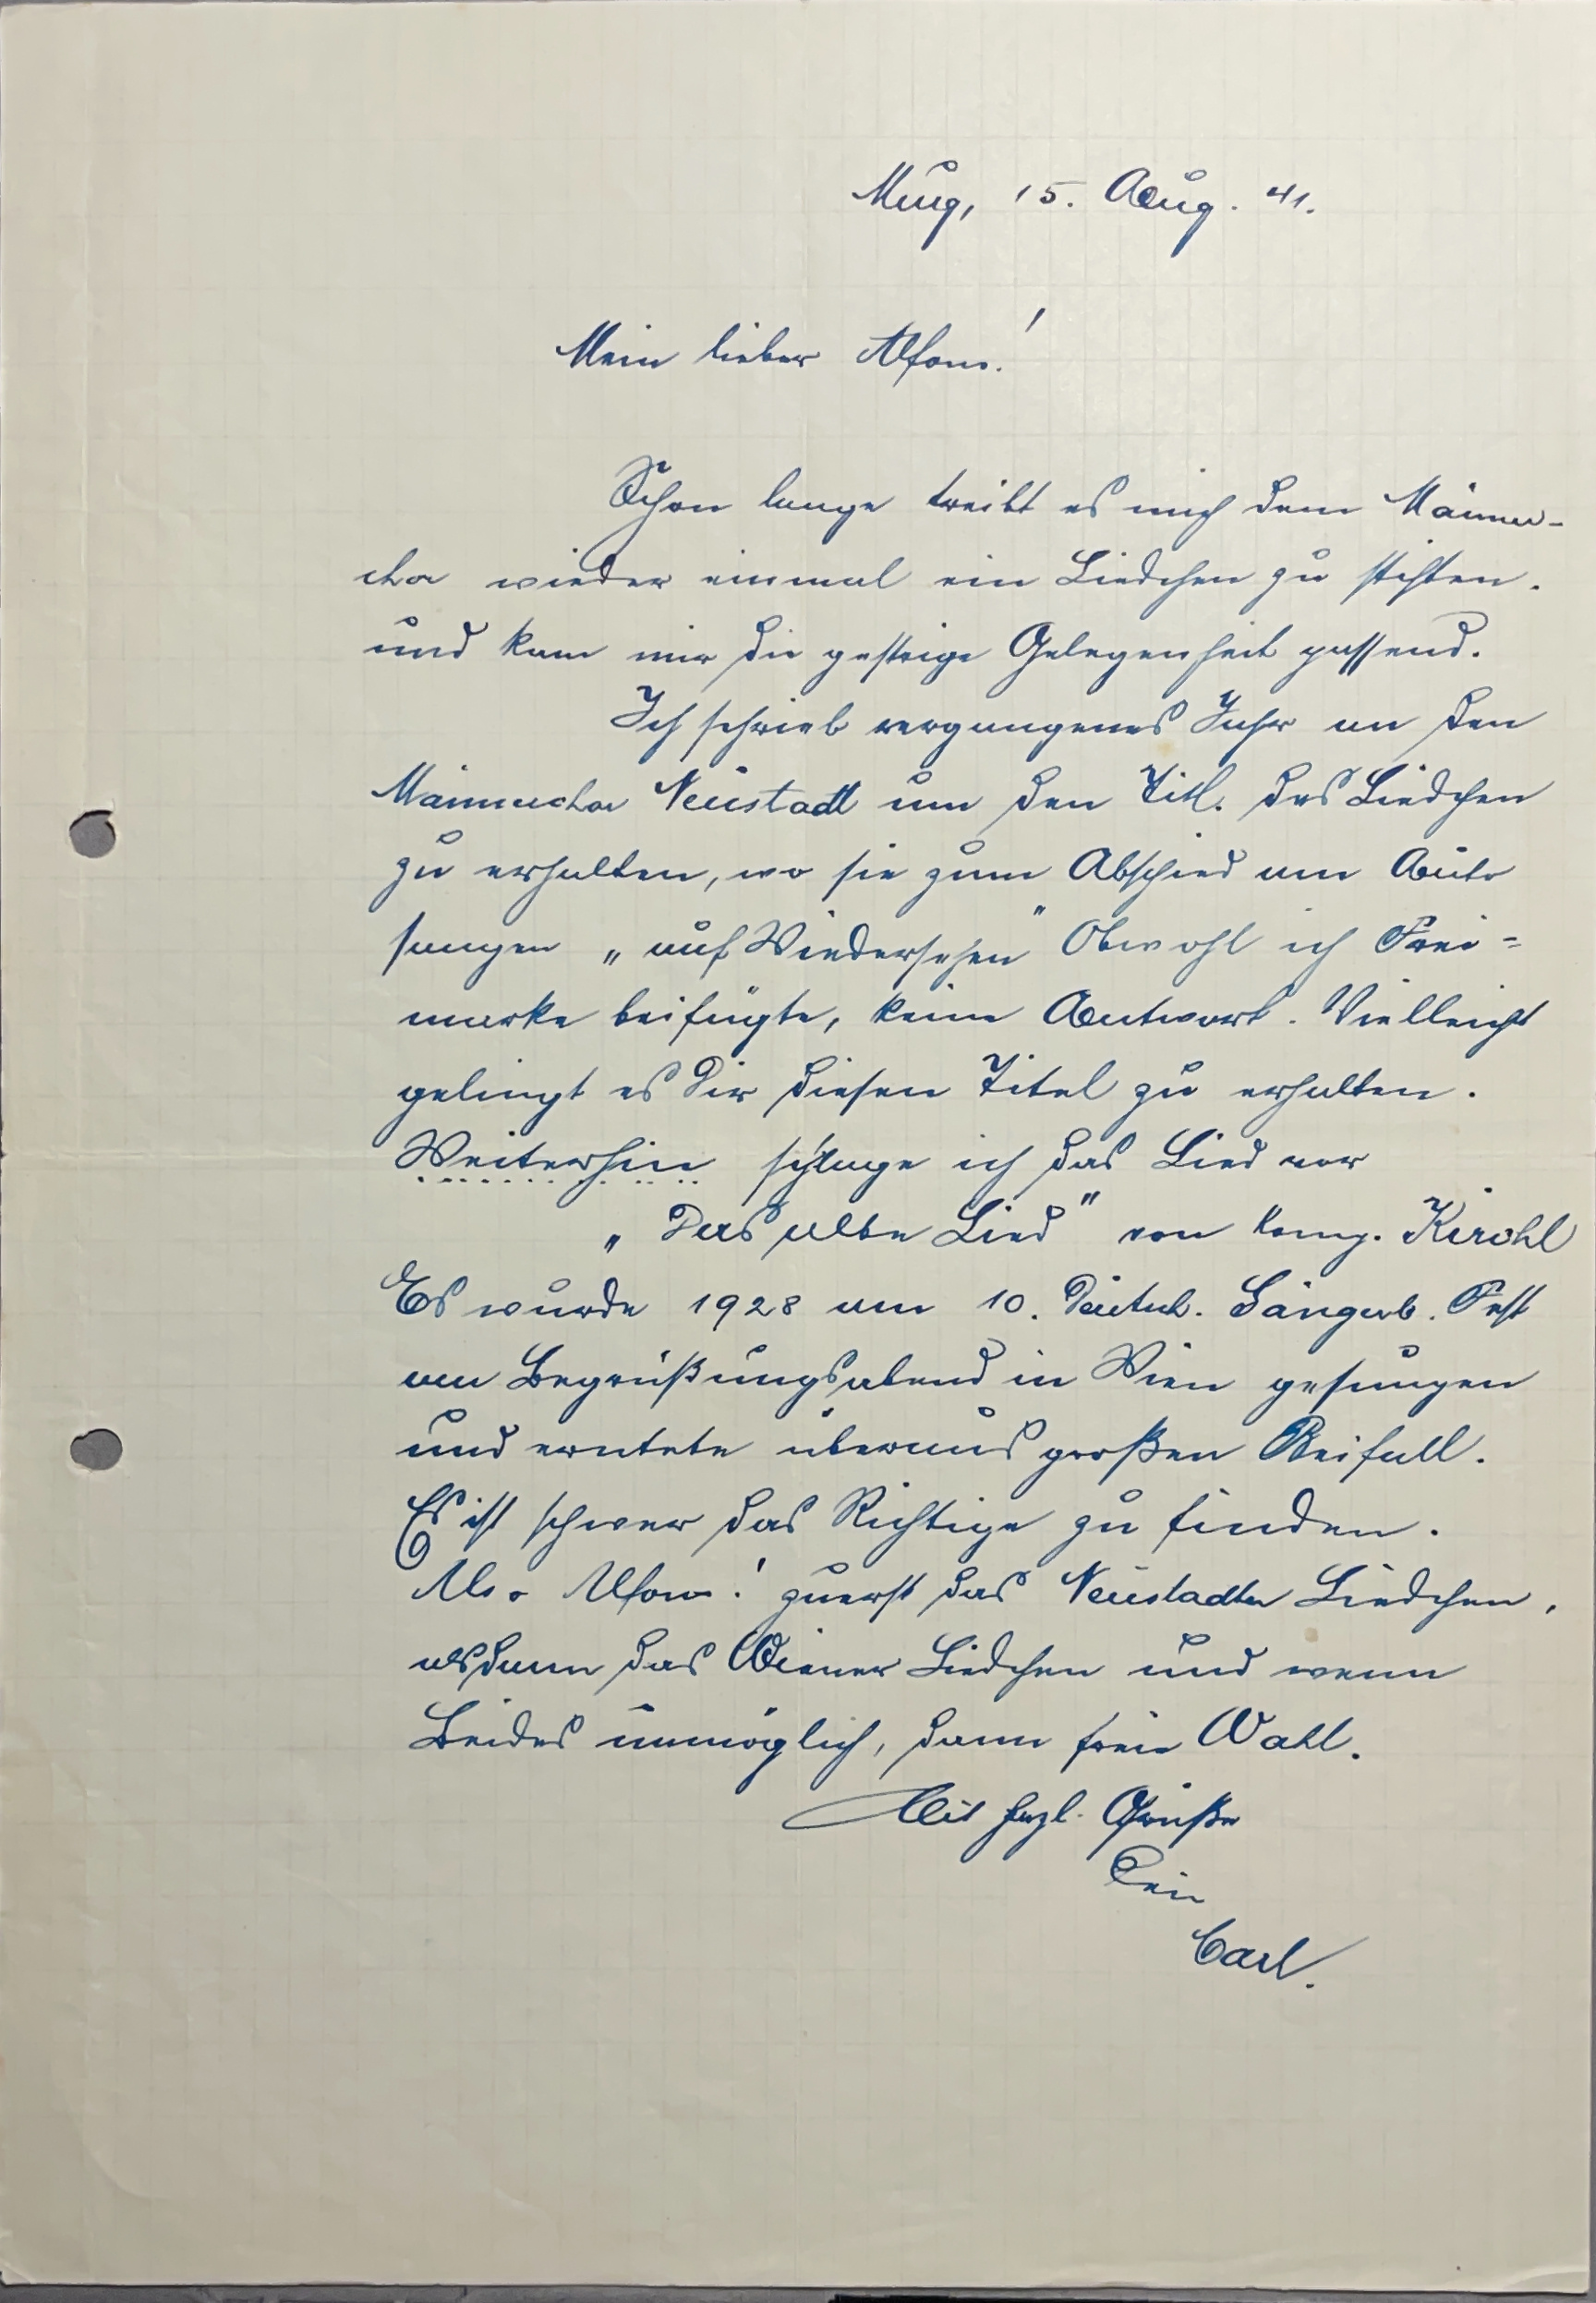
\includegraphics[width=0.8\textwidth]{./assets/Images/Akte_076_S001.jpg}
  \captionof{figure}{Beispiel für handschriftlichen Text in Akte\_076}\label{fig:Carl-handschrift}
\end{minipage}
\vspace{1em}
\footnotetext{Baselines = Schriftausrichtung}

Ausgangspunkt für dieses Projekt ist das generischen Modell \textit{The German Giant I}, 
das mit einer CER\footnote{\textbf{CER} (Character Error Rate): Kennzahl für die Anzahl falsch erkannter Zeichen.} von 8,30\% zunächst auf 70 Akten angewendet wird. 
Sie umfassen 158 Seiten mit insgesamt 22.155 Wörtern. Die Ergebnisse
sind dabei jedoch sehr unpräzise, wie Abbildung \nameref{fig:Carl-Transkribus} veranschaulicht. 
In insgesamt vier Durchläufen über diese Selektion wird daher manuell eine Groundtruth für ein eigenes Modell erstellt und gleichzeitig regelbasiert und strukturiert Personen, Orte, Daten und
Organisationen getaggt. Zwar erweist sich ChatGPT in der direkten Texterkennung aus Bilddateien (OCR) als nicht ausreichend zuverlässig. 




\begin{minipage}[t]{0.52\textwidth}
  \setstretch{1.5}
  \justifying
  \noindent
Wie oben ausgeführt wird zur 
Erstellung des Groundthruth-Korpus bei der manuellen Korrektur OpenAIs ChatGPT-4o-Modell für die Rechtschreibprüfung verwendet. Die vermeintliche Schwäche 
bei der Transkription, passende Begriffe zu halluzinieren, stellen sich als besonders hilfreich heraus. Insbesondere in der Rekonstruktion fehlender Worte oder 
Satzteile aus dem semantischen Kontext heraus Wörter oder Satzteile. 
In Kombination mit der philologischen Expertise bei der Entzifferung einzelner Buchstaben entsteht so ein kollaborativer Transkriptionsprozess, 
bei dem Maschine und Mensch sich wechselseitig ergänzen. Die automatische Transkription wird in \autoref{fig:Carl-Transkribus} dargestellt, die überarbeitete LLM-Version folgt in \autoref{fig:Carl-LLM}.
\end{minipage}
\vspace{1em}
\begin{minipage}[t]{0.5\textwidth}
    \centering
    \vspace*{0cm}
  \begin{tcolorbox}[colback=oldLetter, colframe=black, sharp corners, width=0.8\textwidth]
    \tiny{Murg. 15. Aug 41 
    
    Mein lieber Alfons! 

    Sehen lunge Lreitt es mich dem Männer- 

    chor wieder einmal ein Liedehen zu stehten. 

    und kam mir die gestege Gelegenheit gussend. 

    Männechor Venstad um den Title das Liedchen 

    zu erhalten, wo sie zum Abschied am Aute 

    sängen ``auf Wiederschen Owohl ich Frei! 

    märke beifügte, keine Aentwarb. Vielleicht 

    gelingt es Dir diesen Iitel zu erhalten. 
    
    Weiterhin sänge ich fal Lied nur 
    
    ``Bas alte Lied'' von being. Rerohl 

    Es wurde 1928 am 10. Dachub. Sängerb. Frst 

    von Begrüssungsabend in Dien gesungen. 

    und erntete überaus grossen Reifall. 

    Es ich schwer das Richtige zu finden. 

    Aler Alfon, werst das Vemsladler Liedchen. 

    alsdann das Biener Lidchen und wenn 

    Leides unmöglich, dann freu Nall. 

    Mit herzl. Grüsse 

    Dein 

    Carl} 
  \end{tcolorbox}
  \captionof{figure}{LLM-Version von \autoref{fig:Carl-Transkribus}\label{fig:Carl-LLM}}
\end{minipage}
\hfill%



\begin{minipage}[t]{0.52\textwidth}
  \setstretch{1.5}
  \justifying
  \noindent
Die so entstehnde Groundtruth wird für das Training des Modells
(\href{https://app.transkribus.org/models/public/287793}{ModelID: 287793})\footnotemark{} verwendet.
Dieses trainierte Modell erreicht eine CER von 6,58\% und kommt anschliessend für die automatische Transkription der übrigen Dokumente zum Einsatz. Auch hier ist eine manuelle Überprüfung der durch das eigens trainierte Modell erstellten
Transkription unabdingbar, die knapp 1.7\% geringere CER macht sich jedoch beim Korrekturaufwand bereits bemerkbar. Gleichzeitig wird diese Korrektur für das Taggen benutzt, das folgend beschrieben werden soll.

\end{minipage}
\footnotetext{\cite[vgl.][]{burkhardt_transkribus_2024}}
\begin{minipage}[t]{0.5\textwidth}
    \centering
    \vspace*{0cm}
  \begin{tcolorbox}[colback=oldLetter, colframe=black, sharp corners, width=0.8\textwidth]
\tiny{Murg, 15. Aug. 41

Mein lieber Alfons!

Schon lange treibt es mich, dem Männerchor wieder einmal ein Liedchen zu stiften, und kam mir die günstige Gelegenheit gelegen.

Ich schrieb vergangenes Jahr an den Männerchor Venstad, um den Titel des Liedchens zu erhalten, das sie zum Abschied am Auto sangen: \enquote{Auf Wiedersehen, o wohl ich frei!}

Ich fügte eine Frankierung bei, erhielt jedoch keine Antwort. Vielleicht gelingt es Dir, diesen Titel zu erhalten.

Weiterhin sang ich das Lied nur \enquote{Das alte Lied von Wien}. Obwohl es am 10. Dezember 1928 beim Sängerbund-Fest von Begrüssungsabend in Wien gesungen wurde und überaus grossen Beifall erntete, ist es schwer, das Richtige zu finden.

Aber Alfons, zuerst das Venstadler Liedchen, dann das Wiener Liedchen und wenn beides unmöglich, dann Fröhlichsein.

Mit herzlichen Grüssen

Dein

Carl}

\end{tcolorbox}
  \captionof{figure}{Transkription durch ChatGPT von \autoref{fig:Carl-Transkribus}\label{fig:Carl-LLM}}
\end{minipage}
\hfill%




\subsubsection{Tagging mit Transkribus und LLM}

Während der manuellen Korrektur der Transkriptionen erfolgt parallel die Annotation zentraler Entitäten. 
Transkribus bietet hierfür ein flexibles Tagging-System, mit dem sowohl strukturelle als auch semantische Informationen direkt im Dokument markiert werden können. 
Im Zentrum stehen dabei Tags für Personen, Orte, Organisationen und Datumsangaben. Diese Kategorien sind für die spätere Analyse besonders relevant, 
etwa für die Modellierung historischer Netzwerke oder die Kontextualisierung von Ereignissen.

Ein Mixed-Method-Verfahren kommt dort zum Tragen, wo die Transkription an ihre Grenzen stösst: 
Fehlende Buchstaben, fehlerhafte Worttrennungen oder unleserliche Handschriften lassen sich durch die Kombination aus Modellwissen 
und menschlichem Quellenverständnis rekonstruieren. ChatGPT liefert hier auf Basis des Kontexts plausible Vorschläge, 
die von einer historisch geschulten Bearbeitung geprüft und übernommen oder verworfen werden. Dieser kollaborative Vorgang verbessert 
nicht nur die Lesbarkeit, sondern erhöht auch die semantische Genauigkeit der rekonstruierten Passagen.

Ein Beispiel zeigt die schrittweise Entwicklung einer Transkription: Ausgehend von einem gescannten Originalbrief (\autoref{fig:Carl-handschrift}) 
wird zunächst eine maschinelle Transkription erstellt (\autoref{fig:Carl-Transkribus}), die anschliessend durch ein LLM geglättet und lesbarer gemacht wird 
(\autoref{fig:Carl-LLM}).

In einem letzten Schritt erfolgt die manuelle Annotation mit Transkribus-Tags (\autoref{fig:Tagging-Carl-LLM}): 
Hier werden etwa \texttt{Murg} und \texttt{Wien} als Orte, \texttt{Alfons}, \texttt{Carl} und \texttt{Kirchl} als Personen sowie das 
\texttt{Deutsch. Sängerb. Fest} als Ereignis markiert. Auch der Liedtitel \enquote{Das alte Lied von Wien} wird in seinen Bestandteilen 
zwischen Person, Ort und kulturellem Kontext aufgeschlüsselt. Für unklare oder unleserliche Textstellen, wie etwa das Fragment \texttt{auf Wiederschen}, 
kommt das Tag \texttt{unclear} zum Einsatz – häufig auf Grundlage einer Vorschlagsformulierung durch ChatGPT.
\end{minipage}

Zusätzlich zur semantischen Markierung ermöglicht Transkribus auch die Kennzeichnung struktureller Eigenschaften. 
So wird beispielsweise die Abkürzung \texttt{V.D.A.} – für \textit{Verein für das Deutschtum im Ausland} – mit dem Tag \texttt{abbrev} versehen, 
auch wenn diese Tags in der XML-Exportstruktur teilweise nicht vollständig erhalten bleiben (vgl. Kapitel~\ref{section:Transkriptionen_Methoden}).

Für die spezifischen Anforderungen dieses Korpus wird das Tagging-Schema gezielt erweitert, etwa um den benutzerdefinierten Tag \texttt{signature}, 
der handschriftliche Unterschriften maschinenlesbar ausweist. Das zweite Beispiel – ein poetischer Brief an Otto (\autoref{fig:Tagging-Carl-LLM}, unten) – 
zeigt die Anwendung dieses Verfahrens in lyrischer Sprache. Auch hier werden alle erwähnten Personen (u.\,a. \texttt{Otto}, \texttt{Lina Fingerdick}, 
\texttt{Otto Bollinger}, \texttt{Alfons Zimmermann}), Orte (\texttt{Murg}, \texttt{Laufenburg (Baden)}, \texttt{Rhina}) sowie Organisationen 
(\texttt{Männerchor}) mit den entsprechenden Tags versehen. Die adressierte Funktion \texttt{Vereinsführer des Männerchor} wird dabei 
als Organisationseinheit erfasst und semantisch vom Personenbezug getrennt.

Fehlerhafte oder fehleranfällige Passagen – insbesondere historisch bedingte Schreibungen oder Transkriptionsunschärfen – 
werden mit dem Tag \texttt{sic} versehen. In diesen Fällen folgt die standardisierte Lesart unmittelbar auf das markierte Original, 
wodurch ein differenzierter Umgang mit dem Quelltext sichergestellt ist.

Alle Tags werden während des Transkriptionsprozesses konsistent dokumentiert und in einem projektspezifischen Regelwerk festgehalten. 
Dieses dient nicht nur der internen Nachvollziehbarkeit, sondern auch als Grundlage für die spätere Verarbeitung durch Sprachmodelle, 
die auf die gleichen semantischen Kategorien angewiesen sind. Das strukturierte Tagging bildet somit die Brücke zwischen manueller 
Quellenarbeit und automatisierter Weiterverarbeitung.

% % \begin{itemize}
% %   \item Ausgangslage und technische Bedingungen
% % \item Zeitlicher Verlauf des Digitalisierungsprojekts
% % \item Geräte, Software (iPad, Apple Scan, ökonomische Gründe)
% % \item Mangelnde DH-Vorkenntnisse bei Beginn
% % \item Qualität und OCR-Auswirkungen
% % \item Erste Transkription und Groundtruth-Erstellung
% % \item Nutzung von German Giant I
% % \item Erste Fehleranalyse, CER = 8,3 %
% % \item Auswahl von 70 Akten für manuelle Korrektur
% % \item Iterative Verbesserung in 4 Schritten
% % \item Tagging-Strategie
% % \item Manuelles Tagging von Personen, Orten, Daten, Organisationen
% % \item Ergänzung um Custom-Tags wie \texttt{signature}
% % \item Verwendung von \texttt{sic} für fehlerhafte Vorlagen
% % \item Dokumentation der Regeln zur Weitergabe an LLMs
% % \item Modelltraining und finale Transkription
% % \item Aufbauendes Modell mit CER 6,58 %
% % \item Nutzung des Modells für 80 restliche Akten
% % \item Vorteile im Workflow, aber weiterhin manuelle Kontrolle nötig
% % \item Beispielhafte Ergebnisse (Referenz auf Boxen + Abbildungen)
% % \item Bildquelle → Transkription → korrigierte, getaggte Version
% % \item Beobachtungen: LLM transformiert Inhalt lesbar, aber semantische Fehler (z.B. „Venstad“ vs. „Neustadt“)

% % \end{itemize}

% % Für die Transkrition der Daten wurde ein best-practise Ansatz gewählt. Nach Tests mit dem Python-Modul \textit{\enquote{Tesseract}} 
% % und unterschiedlichen LLMs wurde auf Transkribus zurückgegriffen. Eine Gegenüberstellung der drei erwähnten Tools findet 
% % sich im Kapitel~\nameref{section:Transkriptionen_Methoden}


% \subsection{Tagging}
% blabla
% \subsubsection{Tagging mit Transkribus}
% blabla
% \subsubsection{Tagging mit LLM}
% blabla
% \subsection{Export}
% blabla

%––––––––––––––––––––––––––––––––––––––––––––––––––––––––––––––––––––––––––––––––––––––%
%––––––––––––––––––––––––––––––––––––––––––––––––––––––––––––––––––––––––––––––––––––––%
%––––––––––––––––––––––––           Forschungsstand        ––––––––––––––––––––––%
%––––––––––––––––––––––––––––––––––––––––––––––––––––––––––––––––––––––––––––––––––––––%
%––––––––––––––––––––––––––––––––––––––––––––––––––––––––––––––––––––––––––––––––––––––% 


%––––––––––––––––––––––––––––––––––––––––––––––––––––––––––––––––––––––––––––––––––––––%
%––––––––––––––––––––––––––––––––––––––––––––––––––––––––––––––––––––––––––––––––––––––%
%––––––––––––––––––––––––           Methodisches Vorgehen        ––––––––––––––––––––––%
%––––––––––––––––––––––––––––––––––––––––––––––––––––––––––––––––––––––––––––––––––––––%
%––––––––––––––––––––––––––––––––––––––––––––––––––––––––––––––––––––––––––––––––––––––% 
\section{Methodisches Vorgehen}
\subsection{Genutze Tools}
Digitale Methoden spielen für die Durchführung dieser Arbeit eine zentrale Rolle. Von der Digitalisierung der Quellen
über die Transkription bis hin zur Auswertung durchlaufen die Daten zahlreiche Prozessschritte, die mithilfe von Large 
Language Models, Deep-Learning-Modellen und anderen digitalen Werkzeugen verarbeitet und visualisiert werden. 
Die Auswahl der Tools orientierte sich dabei an Kriterien wie Verfügbarkeit (Open~Source vs.\ proprietär), 
Kompatibilität, Community-Support, erforderlichem Arbeitsaufwand und selbstverständlich dem konkreten Mehrwert für 
die Forschungsfragen.

In diesem Kapitel werden sowohl Werkzeuge vorgestellt, die tatsächlich eingesetzt wurden, als auch solche, die sich 
im Verlauf des Projekts als ungeeignet erwiesen. Transparenz ist hierbei ein wesentlicher Aspekt: Ein grosser Teil der 
Methodik entwickelte sich erst im Forschungsprozess selbst. Da sich Large Language Models rasant weiterentwickeln, 
ist nicht immer von Beginn an klar, ob ein Tool für den eigenen Anwendungsfall geeignet ist.
Um diese Unsicherheiten zu dokumentieren, werden hier auch gescheiterte Versuche dargestellt.

\subsubsection{LOD – Linked Open Data}

Linked Open Data (LOD) bezeichnet einen dezentral organisierten Ansatz zur Veröffentlichung und 
Verknüpfung strukturierter Daten im Web. Ziel ist es, Datensätze verschiedener Institutionen und Akteure 
maschinenlesbar zugänglich zu machen und über standardisierte Formate wie RDF und SPARQL miteinander zu 
verbinden\cite[ vgl.][Preface S. VI \& S. 13f]{garoufallou_metadata_2020}. 
Wesentliches Merkmal der LOD-Cloud ist dabei die Nutzung semantischer Beziehungen, insbesondere Äquivalenzen einzelner Daten. 
Hierfür wird häufig das Prädikat \texttt{owl:sameAs} genutzt, um z.B. mit \colorbox{VeryLightGray}{\textit{:Choir owl:sameAs wd:Q131186}} eine eigene 
Instanz als identisch mit der Wikidata-Entität für einen Chor zu deklarieren.
Klassen oder Instanzen können so aus unterschiedlichen Datenquellen eindeutig identifiziert und zusammengeführt werden.

Die OWL Web Ontology Language, entwickelt vom World Wide Web Consortium (W3C), ist damit ein zentrales Werkzeug für die Realisierung von 
LOD.\cite[ vgl.][]{smith_owl_2004} 
Mit ihr lassen sich Ontologien definieren, die Domänen über Klassen, Individuen und deren Relationen formal beschreiben. 
Sie ermöglichen, logische Schlussfolgerungen zu ziehen, um verteilte Datenbestände zu verknüpfen und maschinenlesbar auszuwerten.
Besonders relevant ist dabei \texttt{owl:sameAs}, das als Identitätsrelation fungiert: 
Es deklariert Instanzen, die in unterschiedlichen Quellen unter verschiedenen URIs\footnote{Abk. \textbf{URI}\: Uniform Resource Identifier} geführt werden, 
als dasselbe reale Objekt\cite[ vgl.][2.3. Data Aggregation and Privacy]{smith_owl_2004}
und ermöglicht so eine präzise Zusammenführung von Informationen — ein Grundpfeiler für die Interoperabilität im Semantic Web.
Die OWL-Spezifikation baut auf RDF\footnote{Abk. \textbf{RDF}\; Resource Description Framework} auf und erweitert es um zusätzliche Konzepte.
Die RDF-Daten werden häufig im Turtle-Format (TTL) serialisiert, einer textbasierten Notation für RDF, die eine kompakte, leicht lesbare Schreibweise bietet.
Dieses Format eignet sich besonders für den Austausch und die manuelle Bearbeitung von RDF-Tripeln.
Die Sprache liegt in drei Varianten vor\footnote{OWL Lite, OWL DL und OWL Full}, die sich im Grad ihrer Ausdrucksstärke 
unterscheiden.\cite[ vgl.][1.1. The Species of OWL.]{smith_owl_2004}
Insbesondere OWL DL bietet einen praktikablen Mittelweg zwischen hoher Ausdruckskraft und vollständigem, entscheidbarem Schliessen (Reasoning) 
und ist daher für viele LOD-Anwendungsfälle geeignet.

Trotz ihres Potenzials wird diese Form der Datenverknüpfung bislang jedoch nicht von allen Websites konsequent 
umgesetzt.\cite[ vgl.][S. 14]{garoufallou_metadata_2020}. Für die technische 
Umsetzung für diese Arbeit werden zwei zentrale Werkzeuge genutzt: Protégé zur Modellierung der Ontologie und GraphDB für deren Verwaltung und Abfrage.

\paragraph{Protégé} Zur praktischen Modellierung der Ontologie kam \textit{Protégé} zum Einsatz. 
Protégé ist eine weit verbreitete Open-Source-Software zur Erstellung, Visualisierung und Verwaltung von Ontologien.
Die grafische Oberfläche unterstützt eine intuitive Klassendefinition, 
Relationserstellung und Instanzverwaltung. 
Mit Hilfe von Plugins können darüber hinaus logische Konsistenzprüfungen durchgeführt und 
Ontologien direkt im OWL-Format exportiert werden, um sie in LOD-Workflows einzubinden.
Die initiale Version der Ontologie für dieses Projekt entstand zuerst im Codeeditor \textit{Visual Studio Code} wurde aber schnell vollständig in Protégé überarbeitet.
Damit bildet das Programm die Grundlage für erste Experimente mit Abfragen in SPARQL.%

\paragraph{GraphDB} Für die Speicherung und Abfrage der Ontologie wurde \textit{GraphDB} verwendet. 
GraphDB ist eine spezialisierte RDF-Triplestore-Datenbank, die es ermöglicht, 
grosse Mengen an semantisch verknüpften Daten effizient zu verwalten. 
Mit der integrierten SPARQL-Schnittstelle können Benutzer gezielt nach Instanzen, Klassen und Relationen suchen 
und komplexe Muster in den Datenbeständen erkennen. 
Im Rahmen dieser Arbeit diente GraphDB als Backend, um die in Protégé entwickelte Ontologie zu testen 
und mit realen Entitäten aus den untersuchten Quellen abzugleichen.



\noindent
\begin{minipage}[t]{0.52\textwidth}
  \setstretch{1.5}
  \justifying%
\paragraph{LOD-Ontologie}\\
Ein wichtiger Aspekt dieser Arbeit ist die Unstrukturiertheit relevanter Informationen. 
Aus diesem Grund wurde auf der Basis der Oben beschrieben Semantik begonnen, eine eigene Ontologie zu entwickeln, die die identifizierten Entitäten systematisch erfasst.
Beim Schreiben dieser initialen Ontologie aus rund 2000 Zeilen Code erweist sich schnell ein neues Problem. Die Datengrundlage aus den geschilderten Vorprojekten (vgl.~\hyperref[subsec:forschungsstand]{Forschungsstand und Forschungslücke}) ist 
zu klein, um daraus eine aussagekräftige Netzwerkanalyse zu machen. Hierfür erweisen sich die Unterschiede der Daten zusätzlich als zu gross tische Grundlage des Globalund damit aufwendig. Der Fokus der Arbeit verschiebt sich dementsprechend von der Ontologieentwicklung 
auf die Extraktion von Entitäten.
\end{minipage}%
\hfill%
  % Rechte Minipage = Bild
  \begin{minipage}[t]{0.43\textwidth}
    \centering
    \vspace*{0.3cm} % ► schiebt alles um 0.3cm nach unten
    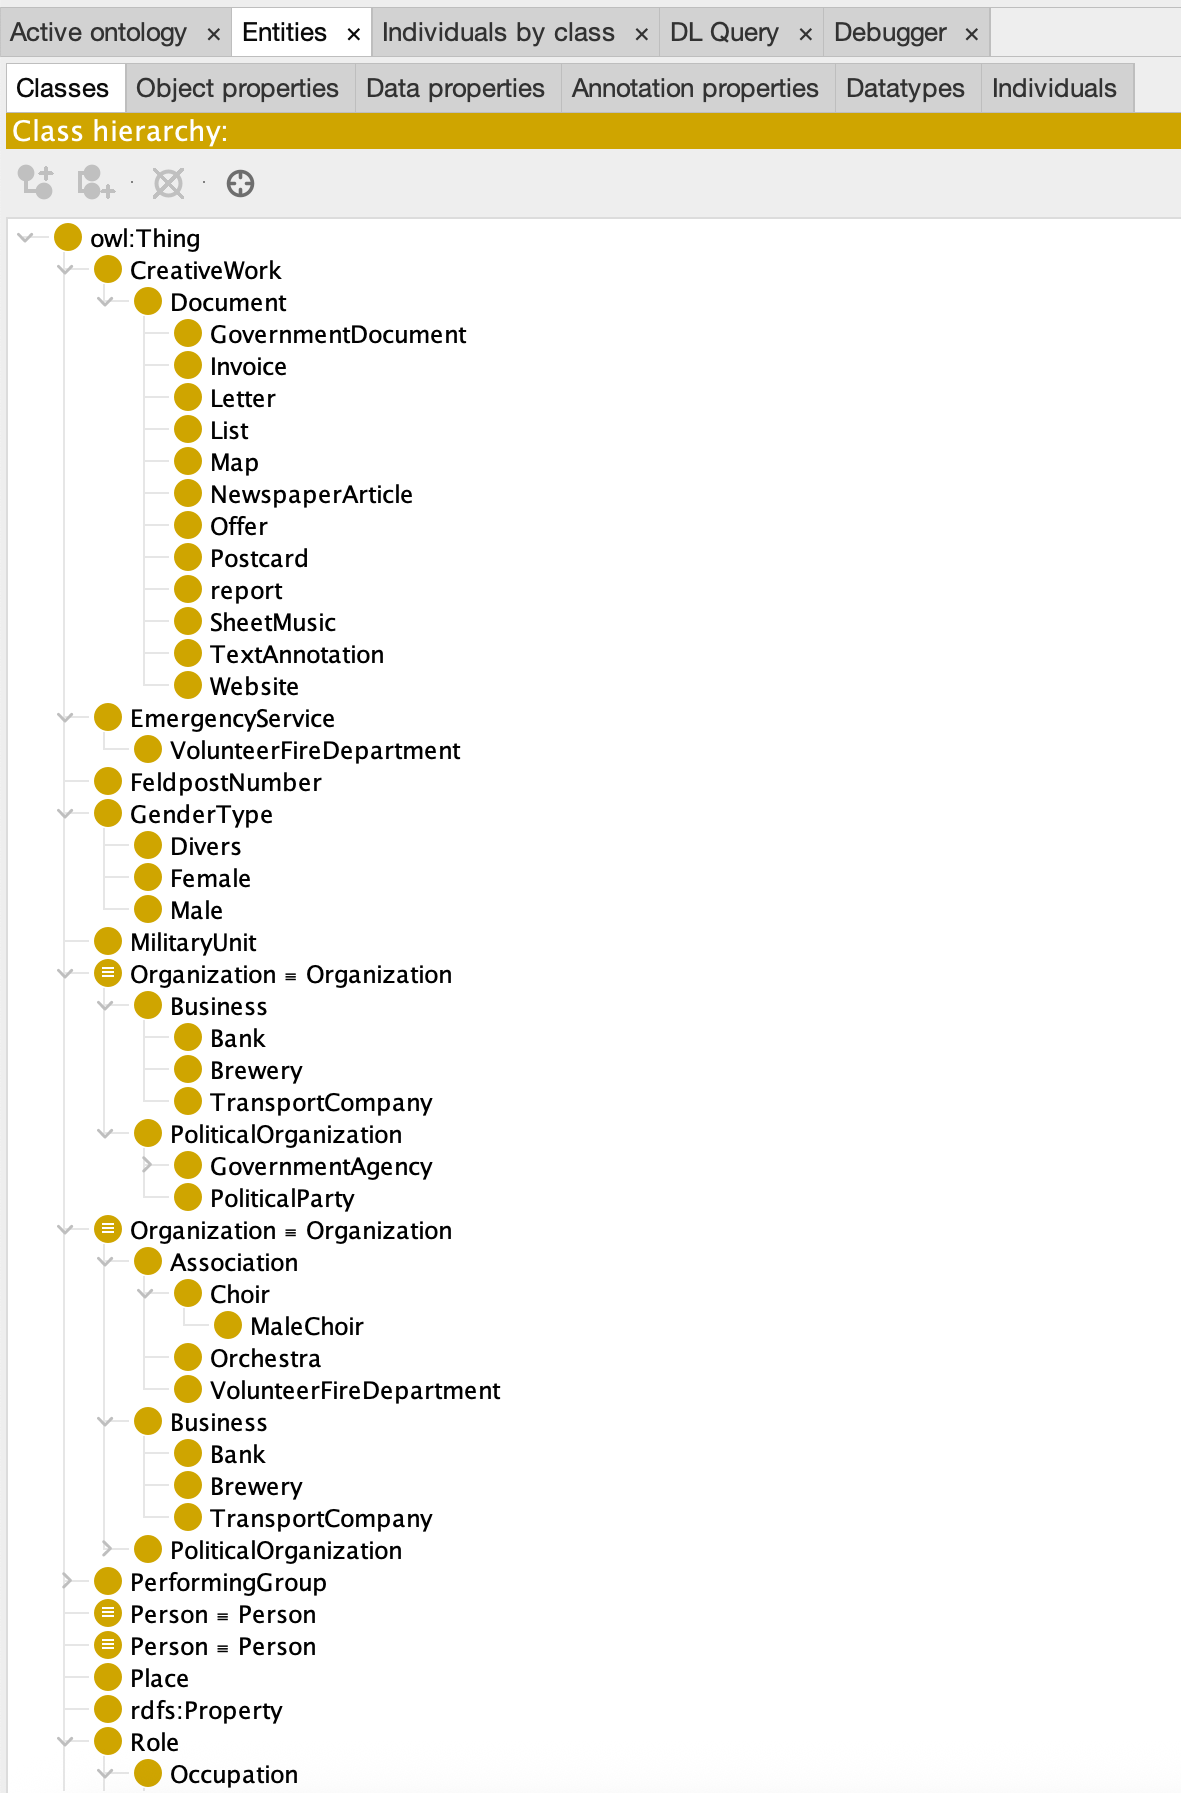
\includegraphics[width=\linewidth]{assets/Images/Bildschirmfoto_ttl_ontologie_Ausschnitt.png}
    \captionof{figure}{Ausschnitt der TTL-Ontologie.}\label{fig:ttl-ontologie}
\end{minipage}

\vspace{1em}

Der bestehende Datensatz ist zu klein, um eine umfangreiche Ontologie lohnend zu machen. Hinzu kommen externe Quellen, und deren Zugänglichkeit. Zuverlässige Quellen für Informationen 
über militärische Einheiten und deren Feldpostnummern sind das \enquote{Forum der Wehrmacht}\cite[ vgl.][]{altenburger_lexikon_nodate} 
und der \enquote{Suchdienst des DRK}\cite[ vgl.][]{reuter_drk_2025}. In beiden Fällen liegen die Daten jedoch nicht als LOD vor, sondern im Forum als einfache Strings 
und beim Deutschen Roten Kreuz als OCR-PDF\footnote{OCR = Optical Character Recognition} historischer Suchlisten aus der Nachkriegszeit. Ein manuelles Recherchieren dieser Daten scheint zu diesem Zeitpunkt
den Rahmen der Arbeit zu sprengen. Die in diesem Schritt geleistete Vorarbeit beim Sortieren und Klassifizieren von Entitäten, besonders in Verknüpfung mit selbst erstellten Wikidata-Klassen 
wird in späteren Prozessschritten wieder aufgegriffen\footnote{siehe Abschnitt~\hyperref[subsec:Nodegoat_chapter]{Nodegoat}}.

\subsubsection{Wikidata}

\textit{Wikidata}\cite[vgl.][]{noauthor_wikidata_nodate} ist eines der zentralen Repositorien für Linked Open Data, und bietet eine hohe Interoperabilität durch standardisierte
URIs, SPARQL-Endpunkte und offene APIs zu den Entitäten.
Jede Entität erhält dabei eine eindeutige, persistente URI 
(z.B. \colorbox{VeryLightGray}{\textit{wd:Q131186}} für einen Chor), die in LOD-Szenarien 
als stabiler Referenzpunkt dient.
Neben anderen betonen Martinez \& Pereyra Metnik (2024) beispielsweise: \\
\textit{\enquote{Wikidata stands out for its great potential in interoperability and its ability to connect data from various domains.}}\cite{martinez_comparative_nodate}

Wikidata entspricht, ebenso wie das nachfolgend beschriebene GeoNames, den FAIR-Prinzipien: Die Daten sind 
\textbf{F}\textit{indable} und \textbf{A}\textit{ccessible}, \textbf{I}\textit{nteroperable} und \textbf{R}\textit{eusable}\cite[ vgl.][S. 2]{wilkinson_fair_2016}.

Im Rahmen dieser Arbeit dient Wikidata als zentrale externe Referenz, um lokal erhobene Entitäten mit international etablierten Datenobjekten 
zu verknüpfen und so ihre Interoperabilität sicherzustellen. Die Plattform ermöglicht eine eindeutige Identifizierung sowie die maschinenlesbare 
Anreicherung um zusätzliche Informationen.

Die praktische Umsetzung zeigt jedoch eine strukturelle Einschränkung. Für diese Arbeiteigens angelegter Einträge auf Wikidata werden
trotz systematischer Verknüpfung mit anderen dort verwalteten Entitäten, etwa mit Armeen, Militäreinheiten, Orten und Personen, entfernt die Community–Moderation etwa 70\% dieser Einträge. 
Das zeigt einerseits hohe internen Qualitätsanforderungen auf, andererseits werden diese jedoch nicht klar kommuniziert. Mit regidem Löschen neuer Einträge wird die Verlässlichkeit und den Nutzen der 
geleisteten Arbeit erheblich begrenzt. 
Aufwand und Unsicherheit über die Persistenz der Einträge machen den ursprünglich vorgesehenen LOD–Ansatz in dieser Form nicht praktikabel.

\subsubsection{GeoNames}\label{subsubsec:geonames}

Ebenso wie Wikidata bietet \textit{GeoNames}\cite[vgl.][]{noauthor_geonames_nodate} eine Open-Source-Plattform für interoperable Daten. GeoNames fokussiert sich hierbei auf geografische Informationen 
und stellt eine umfassende Datenbank mit über 25 Millionen Ortsnamen und rund 12 Millionen eindeutigen geografischen Objekten bereit.  
Alle Einträge sind in neun Feature–Klassen und über 600 spezifische Feature–Codes kategorisiert. Die Plattform integriert Daten zu 
Ortsnamen in verschiedenen Sprachen, Höhenlagen, Bevölkerungszahlen und weiteren Attributen aus unterschiedlichen nationalen und internationalen Quellen.  
Sämtliche Geokoordinaten basieren auf dem WGS84–System\cite[\textit{WGS84: geodätische Grundlage des Global Positioning System (GPS)} ;vgl.][]{noauthor_wgs84_nodate}
und können über frei zugängliche Webservices oder eine API abgerufen werden.  
Darüber hinaus erlaubt GeoNames registrierten Nutzenden, bestehende Datensätze über eine Wiki–Oberfläche zu bearbeiten oder zu ergänzen, wodurch eine 
kollaborative Qualitätssicherung gewährleistet wird.

GeoNames wird in dieser Arbeit intensiv zur Referenzierung von Ortsnamen verwendet und bildet die Basis für die Groundtruth, wie sie in den Kapiteln \nameref{subsec:Nodegoat_chapter} und 
\nameref{subsec:place_matcher_chapter} beschrieben ist. Im Gegensatz zu Wikidata wurde hier von Beginn an darauf verzichtet, eigene Ortsdatensätze zu ergänzen. Dies liegt einerseits an 
den klar kommunizierten Community–Guidelines und andererseits daran, dass der Datensatz bis auf wenige, sehr lokale Flurnamen als nahezu vollständig gelten kann.

Historische Gebäude wie Gaststätten oder Spitäler fehlen folgerichtig in der GeoNames–Datenbank. Diese Lücke ist erwartbar, aber erwähnenswert, da GeoNames 
ansonsten eine nahezu vollständige und ausgesprochen detaillierte Datengrundlage bietet.

\subsubsection{Transkriptionen (Methodenvergleich)}\label{section:Transkriptionen_Methoden}
\paragraph{Tesseract}\label{paragraph:Tesseract}

Da bereits zu Beginn des Projekts klar ist, dass ein Grossteil der Datenverarbeitung mit Python-Code erfolgen soll, wird gezielt 
nach Werkzeugen gesucht, die eine automatische Transkription von gescannten Dokumenten ermöglichen. 
Als besonders etabliert erweist sich ein Open-Source-Projekt zur Texterkennung in Bilddateien, die OCR-Engine Tesseract. 
Tesseract wird seit den 1980er-Jahren entwickelt, zunächst von Hewlett-Packard, später von Google weitergeführt, 
und ist über GitHub öffentlich zugänglich.\cite[vgl.][]{weil_tesseract-ocrtesseract_2025}

Die Software basiert seit Version 4 auf einem LSTM-basierten\cite[Abk.: \textbf{LSTM} steht für \textit{Long Short-Term Memory};  Architektur der frühen Generation rekurrenter neuronaler Netzwerke \textit{RNNs}. LSTMs wurden entwickelt, um Sequenzdaten zu verarbeiten und dabei sowohl kurzfristige als auch langfristige Abhängigkeiten in der Datenfolge zu erfassen – ein typisches Beispiel sind Texte, Sprache, Zeitreihen oder Handschrift. ;vgl.][p.1-2]{beck_review_2020} neuronalen Netzwerk, das besonders bei der Erkennung von zusammenhängenden Textzeilen eine 
hohe Genauigkeit bietet. Tesseract unterstützt neben modernen Schrifttypen auch historische Schriftsätze wie Fraktur, was es besonders geeignet 
für den Einsatz in digitalisierten Archiven macht.\cite[vgl.][]{weil_tesseract-ocrtesseract_2025}

Vorbereitend für den Einsatz von Tesseract müssen alle gescannten PDF in das JPEG Format umgewandelt werden, wofür ein kurzes Python-Script verwendet wird\cite[vgl.][]{burkhardt_githubpdf_to_jpegpy_2025}. 
Im praktischen Einsatz scheiterte die Integration von TEsseract jedoch an der Heterogenität des Korpus: uneinheitliche Layouts, wechselnde 
Schrifttypen, maschinen- und handschriftliche Texte sowie komplexe Textverläufe. Beispielhaft sollen hier überlagerte oder mehrspaltig angeordnete 
Passagen auf Postkarten und Zeitungsartikeln genannt werden, die zu massiven Erkennungsfehlern führten. Auch mit angepassten Segmentierungsparametern (--psm) 
konnte keine zufriedenstellende Texterkennung erzielt werden.

Tesseract wurde daher nicht weiterverwendet.

\paragraph{LLM}\label{paragraph:LLM_transcript}
Analog zum Einsatz des OCR-Systems Tesseract\footnote{siehe Abschnitt \nameref{paragraph:Tesseract}} stellt die Integration von Large Language Models (LLMs) von Beginn an einen zentralen Bestandteil der Projektkonzeption dar.
Aus diesem Grund wird in einer frühen Phase auch der Einsatz von LLMs, spezifisch ChatGPT, bei der Transkription der Unterlagen erprobt.

Der Einsatz von LLMs wie ChatGPT für die Transkription historischer Quellen erweist sich als ambivalent. Während die Modelle nach gezielter 
Anleitung eine erstaunlich präzise Rekonstruktion von Layoutstrukturen und maschinell erfassten Textdaten leisten, bestehen erhebliche Einschränkungen. Im Detail sind das
erhebliche Probleme bei der semantischen Genauigkeit. Das LLM beginnt sehr schnell mit sinnverändernden Haluzinationen, die unklare Textpassagen aus dem gelernten Kontext stimmig auffüllt.
Eine genaue Transkription, mit forcierter Notation von unklaren Stellen\footnote{Beispielsweise durch das Einfügen von \enquote{[\dots]}} gelingt in der Regel nicht. 
Die Verarbeitung handschriftlicher Dokumente scheitert weitgehend und führt zu stark spekulativen oder fehlerhaften Inhalten.

Hinzu kommen zu Projektbeginn technische Begrenzungen: Da ein API-Zugang zu OpenAI noch nicht verfügbar ist, erfolgt der Zugriff 
über die Weboberfläche. Diese stösst bei umfangreichen Eingaben rasch an Kapazitätsgrenzen; 
Sitzungen brechen häufig ab oder lassen sich nicht zuverlässig fortsetzen. Das kann zu inpersistenzen in der Promptstrukturierung und
dem Kontext des LLMs führen, was wiederum direkten Einfluss auf die Verarbeitung der Unterlagen hat.

Zum Zeitpunkt der exploratien Nutzun stelt das zentrales Hindernis der integrierte Content-Filter der Modelle dar. Inhalte mit Bezug zum Nationalsozialismus
führen zu einem sofortigen Abbruch der Verarbeitung. Beispielhaft sollen etwa Grussformeln wie \enquote{\textit{Heil Hitler}} genannt sein. Auffällig ist jedoch, dass
sich diese Filtermechanismen durch alternative Schreibweisen in den Quellen umgehen lassen. Die schreibweise \enquote{\textit{Heil -- Hitler}} umgeht den Filter komplett 
und wird ohne Einschränkung transkribiert.

Ohne den Zugang zur API und dem damit notwendigen Umweg über den Webclient zeigt sich 
zudem, dass LLMs ohne persistente Promptstrukturierung dazu neigen, wichtige Hintergrundinformationen zu vergessen. 
Eine Kombination aus Ground-Truth-gestützter Anleitung und manuellem Review ist daher notwendig, um eine verlässliche Transkription zu gewährleisten. Sie wird in dem Abschnitt \nameref{subsubsec:LLM_use} näher ausgeführt.

Aus den genannten Gründen kommt auch eine Transkription mittels generativem LLM nicht zum Einsatz.

\paragraph{Transkribus}\label{Transkribus}
Transkribus ist eine webbasierte Plattform zur automatisierten Handschrifterkennung (HTR) und Texterkennung (OCR), die sich seit ihrer Entwicklung im EU-Projekt READ 
(Recognition and Enrichment of Archival Documents)\cite[vgl.][]{noauthor_recognition_nodate} als Standardwerkzeug in den digitalen Geschichtswissenschaften etabliert 
hat\cite[vgl.][]{muhlberger_transkribus_2019}. Betrieben wird Transkribus durch die READ-COOP SCE, einer europäischen Genossenschaft.

Die Plattform bietet zwei zentrale Zugriffsmöglichkeiten: einerseits die schlanke Webanwendung \textit{Transkribus Lite}, andererseits den \textit{Expert Client}, 
eine umfangreiche Desktopsoftware zur Bearbeitung und Verwaltung grosser Dokumentenkorpora. Beide Varianten ermöglichen die Transkription von gescannten Dokumenten, 
die Annotation von strukturellen und semantischen Einheiten sowie den Export in verschiedenen Dateiformaten. 

Die Nutzung des Expert Clients erlaubt darüber hinaus eine detaillierte Kontrolle über Transkriptionsprozesse und das zugrunde liegende Datenmanagement. 
Über integrierte Schnittstellen lassen sich grosse Datenmengen effizient verwalten. Auch externe FTP-Clients können zur Anbindung an das interne Dateisystem verwendet werden, 
um beispielsweise umfangreiche Digitalisate in strukturierter Form einzubinden.

Ein zentrales Merkmal von Transkribus ist die Möglichkeit, \textit{Tags} zu vergeben. Diese umfassen sowohl strukturelle Merkmale wie Abkürzungen, Unklarheiten oder Layout-Elemente, 
als auch semantische Einheiten wie Personen, Orte, Organisationen und Daten. Tags können individuell erweitert oder angepasst werden und werden im XML-Export maschinenlesbar dargestellt.

Die Exportfunktion von Transkribus erlaubt den Download der Transkriptionen im standardisierten PageXML-Format. Dieses Format ist auf die langfristige Nachnutzung 
struktureller Informationen ausgelegt und bildet die Grundlage für weiterführende Auswertungsschritte etwa in Digital Humanities-Projekten.

In der praktischen Handhabung zeigt sich jedoch eine teils deutliche Diskrepanz zwischen den im Interface sichtbaren Informationen und der tatsächlichen XML-Ausgabe. 
So werden beispielsweise benutzerdefinierte Abkürzungsauflösungen oder Listenstrukturen nicht zuverlässig im XML ausgegeben. 
Informationen, die manuell innerhalb der Transkriptionsumgebung gepflegt wurden, gehen im strukturierten Export unter Umständen verloren. 
Insbesondere bei Listenobjekten, etwa für Personenverzeichnisse oder Inventare, bleibt die XML-Struktur häufig leer. Eine Möglichkeit zur systematischen Nachbearbeitung 
oder maschinellen Extraktion steht bislang nicht bereit.

Diese Einschränkungen wurden auch in aktuellen Studien festgestellt. So verweisen Capurro et al.\cite[][]{capurro_experimenting_2023} im Rahmen ihrer Analyse mehrsprachiger Handschriftenkorpora 
auf signifikante Herausforderungen bei der automatisierten Layoutanalyse sowie bei der Verarbeitung komplexer Dokumentstrukturen. 
Sowohl beim Tagging als auch bei der Postcorrection sei weiterhin eine umfangreiche manuelle Nachbearbeitung notwendig, um konsistente und weiterverwendbare Datenformate zu erzeugen.

Trotz dieser Limitierungen liegt der methodische Mehrwert von Transkribus insbesondere in der Möglichkeit, ein eigenes HTR-Modell auf Basis einer spezifischen Groundtruth zu trainieren. 
Dies erlaubt es, auf charakteristische Eigenschaften eines konkreten Korpus einzugehen und so die Character Error Rate (CER) gegenüber generischen Modellen deutlich zu reduzieren. 
Darüber hinaus kann durch strukturierte Annotation eine Grundlage für die spätere Modellbewertung oder den Vergleich mit LLM-basierten Verfahren geschaffen werden.

Insgesamt stellt Transkribus eine leistungsfähige Plattform zur initialen Bearbeitung und Annotation historischer Quellen dar. 
Die automatisierte Erkennung unterstützt den Einstieg in umfangreiche Korpora, ersetzt jedoch nicht die editorische Kontrolle und Nachbearbeitung. 
Gerade für forschungsorientierte Projekte mit Fokus auf strukturierte, semantisch angereicherte Daten bleibt eine kritische Auseinandersetzung mit den technischen Grenzen unerlässlich.

\subsubsection{Large Language Models} \label{subsubsec:LLM_use}
Ein zentrales Werkzeug bei der Verarbeitung der historischen Quellen ist die weiter unten näher beschriebene Python-Pipeline, die auf der Verarbeitung von XML-Dateien basiert. Vorgreifend sei erwähnt, dass diese XML-Verarbeitung ein Large Language Model (LLM) zum Custom-Tagging nutzt. Nebst dem Tagging stellt das Programmieren dieser Pipeline eine der Kernherausforderungen dieses Forschungsprojekts dar. 
Für das Tagging und die Entwicklung der Pipeline werden verschiedene Large Language Models intensiv getestet und eingesetzt.
\paragraph{Msty}
Um ein dafür geeignetes LLM zu evaluieren, werden zu Beginn des Projektes beispielhafte Prompts erstellt und deren Ergebnisse systematisch verglichen. Um diesen Vergleich zu erleichtern, wird die Desktop-Anwendung Msty\cite[vgl][]{noauthor_msty_nodate} eingesetzt. Zu den zentralen Funktionen gehören parallele Chatinterfaces (\enquote{Parallel Multiverse Chats}),
eine flexible Verwaltung lokaler Wissensbestände (\enquote{Knowledge Stacks})\cite[vgl][]{noauthor_msty_nodate}, sowie eine vollständige Offline-Nutzung ohne externe Datenübertragung. Msty dient dazu, verschiedene Modelle zu testen, durch die Parallel Multiverse Chats Antworten zu vergleichen und Konversationen strukturiert zu verzweigen und auszuwerten.

Wichtig ist, dass dies kein klassisches Benchmarking auf Basis vergleichbarer Resultate ist. Es wird zu diesem frühen Projektzeitpunkt weder systematisch überpüft, welche Qualität der jeweilge Codeteil hat, noch wird gemessen, wie viel Prozent der Named Entities jeweils richtig erkannt werden. Der direkte Vergleich der getesteten LLMs liefert jedoch schnell ein klares Bild, welches Modell sich am besten eignet. Beprobt werden die Folgenden Anbieter und Modelle:



\paragraph{Alphabet – Gemini}
\paragraph{Anthopic – Claude}
\paragraph{OpenAI – ChatGPT}


\subsubsection{Nodegoat}\label{subsec:Nodegoat_chapter}

Nachdem sich die Implementierung von Linked Open Data (LOD) für das vorliegende Projekt aufgrund des hohen zeitlichen 
Aufwands als nicht realisierbar erwiesen hat, wird mit \textbf{Nodegoat}\cite{kessels_nodegoat_2013}
eine praktikable und zugleich forschungsnahe Alternative eingeführt. Im Folgenden soll das Tool näher beschrieben, und ihre Anwendung für das Projekt erläutert werden.

Nodegoat ist eine webbasierte Plattform, die sich besonders in den Digital Humanities etabliert hat. Es unterstützt Forschende in der Modellierung, 
Verwaltung, Analyse und Visualisierung komplexer Datenbestände. Ein zentrales Merkmal von Nodegoat ist die grafische Benutzeroberfläche, die eine vergleichsweise niedrige Einstiegshürde bietet. 
Auch Forschenden ohne tiefgehende Programmierkenntnisse wird so die Möglichkeit  eröffnet, eigene Datenmodelle zu definieren, zu pflegen und weiterzuentwickeln. 
Die Plattform folgt einem modularen Prinzip: Über das UI\footnote{Abk.:\textbf{UI} User-Interface} können beliebig viele Datenmodelle 
erstellt werden, die sich flexibel an die spezifischen Forschungsfragen anpassen lassen. Diese hohe Individualisierbarkeit der Datenstrukturen erlaubt es, innerhalb kürzester Zeit projektspezifische 
Datenbanken zu konzipieren und fortlaufend zu erweitern oder an sich ändernde Bedürfnisse anzupassen.

Die Grundstruktur eines Modells unterscheidet in Nodegoat zwischen sogenannten \code{Object Descriptions} und \code{Sub-Objects}. 
Erstere legen die grundlegenden Merkmale eines Objekts fest, etwa Zeichenketten, Zahlen oder Verweise auf andere Einträge. 
So kann eine \code{Person} in diesem Projekt neben einem Feld für Vor- und Nachname auch eine Referenz auf ein \code{Gender}-Objekt enthalten, 
das eine eindeutige Geschlechtszuordnung ermöglicht.

Für das hier behandelte Forschungsvorhaben übernimmt Nodegoat die zentrale Verwaltung der Groundtruthdaten, die später als CSV-Export in die Pipeline integriert werden. 
Für die Groundtruth werden folgende Entitäten modelliert:

\begin{table}[h]
  \renewcommand{\arraystretch}{1.5}
  \centering
  \rowcolors{1}{VeryLightGray}{VeryLightGray}
  \begin{tabular}{|p{0.45\textwidth}|p{0.45\textwidth}|}
    \hline
    Personen & Orte \\ \hline
    Organisationen & Ereignisse \\ \hline
    Dokumente & Rollen \\ \hline
    Gender & \\ \hline
  \end{tabular}
  \caption{\small Übersicht der erfassten Entitäten}
\end{table}

Die Auflistung ist dabei so geordnet, dass die Entitäten mit der grössten Anzahl oder Vielfalt an zugehörigen Sub-Objects zuerst genannt werden. \code{Sub-Objects} erlauben eine
noch vielfältigere Abbildung abhängiger Informationen. Das können in dieser Arbeit zum Beispiel Quellenbelege, sowie temporale oder lokale Attribute, die einem Hauptobjekt zugeordnet werden. Lokale Attribute 
werden in Verknüpfung mit \hyperref[subsubsec:geonames]{GeoNames} und für Länder, Flurnamen oder Gewässer im Geojson-Format\cite[Weiterführend:][]{thomson_geographic_2017}. So lassen sich beispielsweise für\code{Persons}
in den Sub-Objekten \code{Geburt} oder \code{Tod} das Datum und der Ort modelieren, sowie die Todesursache notieren.

Die in den Kapiteln \hyperref[section:Transkriptionen_Methoden]{Transkriptionen und Methoden}, \hyperref[subsec:forschungsstand]{Forschungsstand und Forschungslücke} 
sowie \hyperref[subsec:unmatched_logger]{Unmatched Logger} beschriebenen Verarbeitungsschritte bilden die Grundlage für die in Nodegoat hinterlegten Entitäten.
Die strukturierte Erfassung dient dabei nicht nur der internen Qualitätssicherung, sondern ermöglicht auch eine nachhaltige Referenzierbarkeit durch eindeutig 
vergebene Identifikatoren, die beispielsweise beim Abgleich von Personendaten genutzt werden, um Textstellen präzise mit den zugehörigen Datenbankeinträgen zu verknüpfen.

Darüber hinaus wird Nodegoat über seine Programmierschnittstelle (API) mit einer eigens entwickelten Webanwendung verknüpft. Diese Webanwendung fungiert als publikumsorientierte 
Such- und Präsentationsplattform für die erarbeiteten Quellen. Die in den strukturierten JSON-Daten enthaltenen Nodegoat-IDs verknüpfen hier ebenfalls jede identifizierte Named Entity eindeutig mit dem 
zugehörigen Objekt in der Nodegoat-Datenbank. Dies soll nachfolgend erläutert werden.

Kritisiert werden muss an Nodegoat die fehlende Doukumentation. Viele Informationen finden sich nur über Drittparteien\cite[beispielsweise durch Schulungsunterlagen von Universitäten, 
hier besonders:\\][]{gubler_nodegoat_nodate} oder, wie unten geschildert, auf konkrete Nachfrage bei den Entwicklern. Der dann geleistete Support 
ist jedoch ausgesprochen zeitnah und umfassend. 



\subsubsection{\colorbox{red}{Webtool}}\label{subsec:webtool_chapter}
Die Planung sieht vor, oben beschriebene Verknüpfung zu nutzen, um aus der Webanwendung heraus bei Bedarf Detailinformationen zu den einzelnen Entitäten abzurufen. 
Dazu wird über spezifische API-Requests die jeweilige Objektbeschreibung geladen. In einem exemplarischen Anwendungsfall wird etwa eine Abfrage an eine URL der Form
\begin{figure}
  \hspace*{-0.6cm}%
  \centering\code{https://api.nodegoat.dasch.swiss/data/type/\colorbox{MediumGray}{11680}object/ngEL9c68pELQqGVuoFN49t/}
\end{figure}
gesendet. Hierbei steht die Type-ID \textit{11680} im Beispiel für den jeweiligen Modelltyp \enquote{Organisation} und die Zeichenkette am Ende für die eindeutige Nodegoat-ID 
des Objekts\footnote{im Beispiel eine gekürzte Nodegoat-ID}.

Die dabei zurückgelieferte JSON-Antwort enthält die gespeicherten Metadaten (z.B. Namensvarianten, Zugehörigkeiten, Quellenbelege). Um diese Informationen benutzerfreundlich darzustellen, 
wird angestrebt, den aus Nodegoat bekannten \enquote{Object Detail View} in Form eines iFrames direkt in die Webanwendung einzubetten. Dabei kann über gezielte CSS-Regeln gesteuert werden, dass 
lediglich der gewünschte Objektbereich angezeigt wird, ohne die übrigen Bestandteile der öffentlichen Nodegoat-Oberfläche zu übernehmen.

In der technischen Umsetzung wurde zudem erörtert, ob die interne Object-ID oder die plattformübergreifende Nodegoat-ID als Referenz verwendet werden sollte. Die Rückmeldung bei den
Nodegoat-Entwicklern (Kessels und van Bree) legt auf Anfrage nahe, dass beide ID-Typen im Prinzip austauschbar sind: Die Object-ID gewährleistet eine eindeutige Identifikation 
innerhalb einer spezifischen Nodegoat-Instanz, 
während die Nodegoat-ID eine konsistente Referenz über mehrere Installationen hinweg ermöglicht — auch im Hinblick auf LOD-Kompatibilität.

Für die Integration in die eigene Webanwendung wird daher ein hybrides Modell verfolgt: In den JSON-Daten der Quelltexte werden Nodegoat-IDs gespeichert, um langfristig eine offene Verknüpfbarkeit sicherzustellen. 
Gleichzeitig wird über die API der jeweilige Objekttyp (z.B.\enquote{Person}, \enquote{Organisation}) abgefragt, um die semantischen Eigenschaften der Entität zu laden. Diese werden mit dem 
Model-Endpunkt kombiniert (z.B. \code{https://api.nodegoat.dasch.swiss/model/type/11680}), um etwa Labelstrukturen oder benutzerdefinierte Felder korrekt abzubilden.

Auf diese Weise kann die Webanwendung den Nutzenden nicht nur eine reine Objektliste liefern, sondern auch kontextreiche Detailansichten generieren. Sie sind als iFrame eingebettet oder dynamisch 
gerendert und visualisieren alle relevanten Informationen direkt aus Nodegoat. Um die Serverlast zu minimieren, wird hierbei eine Caching-Strategie empfohlen, sodass wiederholte API-Abfragen 
effizient verarbeitet werden können.

Zusammengefasst fungiert Nodegoat somit als zentrales Bindeglied zwischen der internen Datenhaltung und der öffentlichen Präsentation: Es vereinfacht die Pflege konsistenter Groundtruth-Daten, 
unterstützt deren Ausspielung über standardisierte Schnittstellen und ermöglicht eine modular erweiterbare Verknüpfung mit Webportalen und Suchsystemen.



\subsection{Netzwerkanalyse als Methode}
  \subsubsection{Theoretischer Hintergrund der Netzwerkanalyse}
  \subsubsection{Ziele der Netzwerkanalyse im Kontext der Quellen}
  \subsubsection{Technische Umsetzung (Tools, Datenbankstruktur)}



%––––––––––––––––––––––––––––––––––––––––––––––––––––––––––––––––––––––––––––––––––––––%
%––––––––––––––––––––––––––––––––––––––––––––––––––––––––––––––––––––––––––––––––––––––%
%––––––––––––––––––––––––––––––––––––––––––––––––––––––––––––––––––––––––––––––––––––––%
%––––––––––––––––––––––––           Pipeline        ––––––––––––––––––––––%
%––––––––––––––––––––––––––––––––––––––––––––––––––––––––––––––––––––––––––––––––––––––%
%––––––––––––––––––––––––––––––––––––––––––––––––––––––––––––––––––––––––––––––––––––––% 
\section{Pipeline}
\subsection{Vorverarbeitung}
Neben Transkribus, das bei der Transkription einen elementaren Schritt in der Vorverarbeitung aller Dokumente darstellt,
müssen die Seiten noch weiter vorbereitet werden, um detaillierte Ergebnisse zu gewinnen. Die Kernherausforderung der vorliegenden Arbeit ist die Named Entity Recognition. Wie bereits 
im Abschnitt \nameref{Transkribus} ausgeführt, werden viele Inhalte bereits während des Transkriptionsprozesses manuell getaggt. 
Aufgrund der Menge
an Unterlagen und des begrenzten zur Verfügung stehenden Zeitrahmens wird für das Projekt auch eine zweite Verarbeitungsform gewählt.

Im Zentrum des Vorverarbeitungsskripts steht eine strukturierte Anbindung an die OpenAI-API, um ausgewählte 
PAGE-XML-Dateien aus dem Transkribus-Export automatisiert mit Annotationen anzureichern. Das Skript ist modular
 aufgebaut und folgt einer klar definierten Abfolge von Verarbeitungsschritten, die im Folgenden näher erläutert werden.

Zunächst wird mit der Funktion \code{get\_api\_client()} eine Verbindung zur OpenAI-Programmierschnittstelle 
aufgebaut. Dabei wird der API-Schlüssel über eine Umgebungsvariable geladen und für spätere Anfragen bereitgestellt.
Die zentrale Annotation erfolgt in der Funktion \code{annotate\_with\_llm()}, die den vollständigen Unicode-Text der XML-Datei
verarbeitet und an das Modell GPT-4o übergibt. Grundlage ist ein präzise formulierter Prompt, der die Struktur des zu erwartenden
Outputs definiert. Der Prompt spezifiziert, dass ausschliesslich \code{<TextLine>}-Elemente bearbeitet und mit einem \code{custom}-Attribut
versehen werden dürfen. Innerhalb dieses Attributs werden ausschliesslich tatsächlich erkannte Entitäten in standardisiertem Format codiert, 
darunter Personen (\code{person}), Rollen (\code{role}), Orte (\code{place}), Organisationen (\code{organization}), Daten (\code{date}) 
sowie autoren- und empfängerbezogene Markierungen (\code{author}, \code{recipient}, \code{creation\_place}). Für jedes einzelne Tag gibt es genaue Anweisungen
an das Modell. Auch ein Beispielresultat der Anotation wird jedes mal mitgeliefert, um möglichst wenig Varianz in den Antworten zu erhalten. Gleichzeitig liefert
das Beispielresultat auch Informationen über Abkürzungen, die nicht von dem Modell als Organisationen erkannt werden. Das \enquote{WhW - das Winterhilfswerk} ist eine
abkürzung, die offenbar nicht in den Trainingsdaten des Modells vorkommt. Dieses Vorgehen stellt den Versuch dar, ein nicht domänenspezifisch trainiertes Modell 
auf eine historische Quellenlage zu adaptieren. Es ist jedoch davon auszugehen, dass ein speziell auf den historischen Korpus abgestimmtes Sprachmodell 
deutlich präzisere Ergebnisse liefern würde.

Die Antwort des Sprachmodels ist eine vollständige XML-Datei, die sämtliche bestehenden Strukturinformationen beibehalten soll. 
Der Rückgabewert wird zunächst in der Funktion \code{clean\_llm\_output()} auf mögliche Formatierungen überprüft. Diese Funktion 
extrahiert den tatsächlichen XML-Inhalt aus dem Rückgabestring, etwa wenn dieser durch Markdown-Wrapper wie \code{\texttt{\char\`{}\`{}xml-content\'{}\'{}\'{}}
} eingefasst wurde. 

Die konkrete Verarbeitung einzelner Dateien erfolgt über die Funktion \code{process\_file()}, die eine originale Transkribus-XML-Datei einliest,
an das Modell übergibt, das Ergebnis prüft und anschliessend unter verändertem Dateinamen (Suffix \code{\_preprocessed}) abspeichert. Vor dem 
Schreiben erfolgt eine strukturelle Validierung mittels XML-Parser, um syntaktische Fehler oder unvollständige Rückgaben zu 
erkennen. Fehlermeldungen werden protokolliert, fehlerhafte Dateien übersprungen.

Die eigentliche Ausführung der Batch-Verarbeitung wird durch die \code{main()}-Funktion gesteuert. Diese durchläuft das in 
\code{TRANSKRIBUS\_DIR} konfigurierte Arbeitsverzeichnis, wobei alle Unterordner der Form \code{<7-stelliger Ordner>/Akte\_<Nummer>/page/} 
rekursiv analysiert werden. XML-Dateien, die bereits mit \code{\_preprocessed} enden, werden übersprungen. Zusätzlich wird ein Verzeichnis 
ignoriert, wenn bereits mehr als fünfzig Prozent der Dateien annotiert wurden. Die verbleibenden Dateien werden schrittweise mit dem Modell 
verarbeitet. Hintergrund ist eine kosteneffiziente Verarbeitung, die verhindern soll, dass Datein mehrfach durch die API bearbeitet werden. Die Funktion 
\code{annotate\_with\_llm()} berechnet darüber hinaus die Anzahl der vom Modell verarbeiteten Eingabe- und Ausgabetokens. Auf Basis dieser Werte wird für 
jede Datei eine Schätzung der anfallenden API-Kosten vorgenommen. Diese Informationen werden für jede Anfrage protokolliert, um eine transparente 
Kostenkontrolle sicherzustellen.

Am Ende dieses Prozesses entsteht pro annotierter Seite eine neue, syntaktisch validierte XML-Datei, 
die alle Annotationen als \code{custom}-Attribute enthält. Diese dienen in den nachfolgenden Modulen der 
ipeline (insbesondere \code{transkribus\_to\_base.py}) als Grundlage für die strukturierte Extraktion und Validierung von Entitäten.

\subsection{Aufbau XML to JSON Pipeline}
\subsubsection{Übersichtsgrafik der Pipeline}
\vspace{6\baselineskip}
\begin{figure}[htbp]
  \centering
  \resizebox{0.9\textwidth}{!}{
    \begin{tikzpicture}[
  module/.style={rectangle, draw=black, fill=blue!10, thick, minimum width=4.5cm, minimum height=1.2cm, align=center},
  process/.style={rectangle, draw=black, fill=orange!20, thick, minimum width=4.8cm, minimum height=1.2cm, align=center},
  source/.style={rectangle, draw=black, fill=green!30!gray!20, thick, minimum width=4.2cm, minimum height=0.7cm, align=center},
  group/.style={draw=gray, dashed, rounded corners, inner sep=0.5cm},
  arrow/.style={-Latex, thick}, arrowboth/.style={<Latex>-<Latex>, thick},
  node distance=0.8cm and 1.6cm
]


% --- Hauptquellen oben ---
\node[source] (transkribus) at (-14.5, 0) {\textbf{app.transkribus.org} \\ Transkription};
\node[process] (dir) at (0, -3.2) {\textbf{Dateiverzeichnis} \\ mit XML-Dateien};
\node[process] (llmpre) at (6, -3.2) {\textbf{llm\_XML\_preprocessing.py}};
\node[process, below=7.5cm of dir] (main) {\textbf{Transkribus\_II\_Test.py} \\ Hauptverarbeitung};

% ------------------- MODULE (FLOWCHART) ------------------------
\node[module, below=2cm of main] (init) {Initialisierung \\ (CSV-Import, Matcher)};
\node[module, below=of init]    (xml)  {XML \& Custom-Tags \\ Parsen, extract\_metadata};

% Referenzpunkt zentriert unter xml
\coordinate (modcenter) at ($(xml.south) + (0,-1.8)$);

\node[module] (roles)   at ($(modcenter) + (-8cm, -0.5)$) {Rollen \\ zuweisen, anreichern};
\node[module] (persons) at ($(modcenter) + (-2.7cm, -0.5)$) {Personen \\ match, split, enrich};
\node[module] (orgs)    at ($(modcenter) + (2.7cm, -0.5)$)  {Organisationen \\ extrahieren, deduplizieren};
\node[module] (places)  at ($(modcenter) + (8cm, -0.5)$)  {Orte \\ Kontext + Kombination};
\node[module] (dates)  at ($(modcenter) + (13cm, -0.5)$) {Daten \\ combine\_dates(), count};
\node[module] (events)  at ($(modcenter) + (-13.5cm, -0.5)$)  {Events \\ extract\_events\_from\_xml()};
\node[module, below=1.2cm of persons] (authors) {Autoren \& Empfänger \\ infer, dedup, score};
\node[module] (unmatched) at ($(modcenter) + (0cm, -7.5cm)$) {unmatched\_logger.py};
\node[module] (json)  at ($(modcenter) + (0cm, -9.5cm)$)  {BaseDocument Build \\ + Rollenpostprocessing};
\node[coordinate] (joinpoint) at ($(unmatched.north) + (0, 1.5cm)$) {};
\node[coordinate] (joinpointxml) at ($(xml.south) + (0, -0.5cm)$) {};
\node[source, below=of json] (save) {Speicherung \\ JSON pro Seite + total\_json};
\node[source, right=of save] (unmatchedjson) {unmatched.json};

% CSV-Quellen
\node[source] (csv1) at ($(transkribus.south) + (0.5, -4.5)$) {\textbf{export-person.csv}};
\node[source, below=0.6cm of csv1] (csv2) {\textbf{export-place.csv}};
\node[source, below=0.6cm of csv2] (csv3) {\textbf{export-roles.csv}};
\node[source, below=0.6cm of csv3] (csv4) {\textbf{export-organisationen.csv}};

\node[group, fit=(csv1)(csv2)(csv3)(csv4), name=nodegoatbox,
  label={[anchor=north west, xshift=-0.5cm, yshift=0.7cm]north west:\texttt{Vorverarbeitung: Nodegoat-Exporte}}] {};

\node[group, fit=(transkribus), name=pretranskribusbox,
  label={[anchor=north west, xshift=-0.5cm, yshift=0.7cm]north west:\texttt{Vorverarbeitung: Transkribus}}] {};

 %--- Gruppenrahmen für Modulblock ---
\node[group, fit=
  (persons)(authors)(roles)
  (orgs)(dates)(events)
  (places)(joinpoint), name=flowchartbox] {};

% --- Gruppenrahmen um Hauptverarbeitung + Flowchart ---
\node[group, fit=(main)(flowchartbox)(save),
  label={[anchor=north west, xshift=12.5cm, yshift=+0.7cm]north west:\texttt{Hauptverarbeitung der Transkribus\_II-Pipeline}}] {};


% Verbindungen
\draw[arrow] (transkribus.east) -- ++(1.2,0)-- ++(0,-3.2)-- node[pos=0.6, left, font=\small, xshift=-2cm, yshift=1.3cm]{\textit{Export als XML}} (dir.west);  
\draw[arrow] (dir.east) -- (llmpre.west);
\draw[arrow] (llmpre.north) -- ++(0,1.2) -| node[pos=0.5, above, font=\small, xshift=3cm] {\textit{Custom-Tags}} (dir.north);
\draw[arrow] (dir.south) -- (main.north);
\draw[arrow] (main.south) -- (init.north);
\draw[arrow] (init.south) -- (xml.north);

\draw[arrow] (xml.south) -- (joinpointxml.south);
\draw[arrow] (joinpointxml) -- ($(roles.north |- joinpointxml)$) -- (roles.north);
\draw[arrow] (joinpointxml) -- ($(persons.north |- joinpointxml)$) -- (persons.north);
\draw[arrow] (joinpointxml) -- ($(orgs.north |- joinpointxml)$) -- (orgs.north);
\draw[arrow] (joinpointxml) -- ($(places.north |- joinpointxml)$) -- (places.north);
\draw[arrow] (joinpointxml) -- ($(dates.north |- joinpointxml)$) -- (dates.north);
\draw[arrow] (joinpointxml) -- ($(events.north |- joinpointxml)$) -- (events.north);
\draw[arrow] (unmatched.east) -- ($(unmatchedjson.north |- unmatched.east)$) -- (unmatchedjson.north);

\draw[arrow, dashed] (persons.south) -- (authors.north);
\draw[arrow] (persons.west) -- (roles.east);
\draw[arrow] (roles.east) -- (persons.west);   
\draw[arrow] (persons.east) -- (orgs.west);
\draw[arrow] (orgs.west) -- (persons.east); 
\draw[arrow] (persons.east) -- (orgs.west);
\draw[arrow] (orgs.west)-- (persons.east)  ;      
\draw[arrow] (orgs.east) -- (places.west);  
\draw[arrow] (places.west) -- (orgs.east);  

             
% Doppelte Pfeile mit definiertem Stil
\draw[arrow] (events.south) -- ($(events.south |- joinpoint)$);
\draw[arrow] ($(events.south |- joinpoint)$) -- (joinpoint);

\draw[arrow] (roles.south) -- ($(roles.south |- joinpoint)$);
\draw[arrow] ($(roles.south |- joinpoint)$) -- (joinpoint);

\draw[arrow] (authors.south) -- ($(authors.south |- joinpoint)$);
\draw[arrow] ($(authors.south |- joinpoint)$) -- (joinpoint);

\draw[arrow] (orgs.south) -- ($(orgs.south |- joinpoint)$);
\draw[arrow] ($(orgs.south |- joinpoint)$) -- (joinpoint);

\draw[arrow] (places.south) -- ($(places.south |- joinpoint)$);
\draw[arrow] ($(places.south |- joinpoint)$) -- (joinpoint);

\draw[arrow] (dates.south) -- ($(dates.south |- joinpoint)$);
\draw[arrow] ($(dates.south |- joinpoint)$) -- (joinpoint);

\draw[arrow] (joinpoint.south) -- (unmatched.north);


\draw[arrow] (json.south) -- (save.north);
\draw[arrow] 
  (nodegoatbox.south) |- ([xshift=-0.4cm]init.west)
  node[pos=0.6, left, font=\small, xshift=2.6cm, yshift=2.8cm]{\textit{liefert Groundtruth}};
\end{tikzpicture}
  }
  \caption{Übersicht der gesamten XML-to-JSON-Pipeline}\label{fig:pipeline-uebersicht}
\end{figure}
\vspace{6\baselineskip}


\subsection{Hauptmodul -- transkribus\_to\_base}\label{sec:transkribus_to_base}
\subsubsection*{1. Initialisierung und Pfadlogik}

Die Initialisierungsphase des Skripts\footnote{bis ca. Line 250} dient der Einrichtung sämtlicher Systempfade, Datenquellen, 
Modulabhängigkeiten und Ressourcen. Im Zentrum steht dabei die Festlegung der Projektstruktur sowie die dynamische Integration 
aller untergeordneten Module und Datenbestände.

Zu Beginn werden die Python-Standardbibliotheken sowie externe Abhängigkeiten geladen, darunter \code{pandas} für 
Tabellenverarbeitung, \code{spacy} für die linguistische Analyse und \code{rapidfuzz} für den Vergleich von ähnlichen Strings. Zusätzlich 
wird das aktuelle Datum mit Zeitstempel generiert und als Konsolenoutput ausgegeben. Das unterstützt die Nachvollziehbarkeit von
Verarbeitungsläufen und das Debugging in größeren Verarbeitungsszenarien.

Das Verzeichnis der Skriptdatei wird mithilfe des \code{pathlib}-Moduls identifiziert. Anschließend wird von dort ausgehend das 
Projektwurzelverzeichnis nachvollzogen. Diese dynamisch bestimmte Wurzel fungiert als zentraler Referenzpunkt für die Auflösung 
aller nachfolgenden Verzeichnispfade, absolute Pfadangaben werden vollständig vermieden.  
Das Projekt ist so organisiert, dass sämtliche zentralen Datenverzeichnisse, Ressourcen und Modulstrukturen relativ
zur Wurzel definiert und im Code programmatisch zugänglich gemacht sind. Dazu gehören beispielsweise die 
Unterverzeichnisse \code{Data} für CSV-basierte Groundtruth-Informationen, \code{Module} für modulare 
Verarbeitungsfunktionen sowie \code{Transkribus\_test\_In} und \code{Transkribus\_test\_Out} als standardisierte 
Ein- und Ausgabeverzeichnisse für XML-Dateien und strukturierte JSON-Outputs.

Zur Gewährleistung der Modulverfügbarkeit wird dem globalen Importpfad das Verzeichnis \code{Module} über \code{sys.path.insert} hinzugefügt. 
Dadurch lassen sich alle enthaltenen Funktions- und Klassendefinitionen zentral importieren. Die einzelnen Komponenten sind in 
modularisierten Unterdateien wie \nameref{subsec:person_matcher.py}, \nameref{subsec:place_matcher_chapter} und \nameref{subsec:document_schema} abgelegt. 
Diese Struktur fördert die klare Trennung thematischer Verantwortlichkeiten innerhalb des Codes.

Darüber hinaus erfolgt die Definition aller relevanten Ein- und Ausgabepfade. Der 
Pfad \code{TRANSKRIBUS\_DIR} verweist auf das Eingabeverzeichnis für XML-Dateien, während 
\code{OUTPUT\_DIR} die Ausgabe der JSON-Dateien sowie untergeordnete Strukturen für nicht 
gematchte Entitäten, Logdateien und CSV-Dumps aufnimmt.

Die Initialisierungslogik umfasst ferner das standardisierte Einlesen der Groundtruth-Dateien aus den 
jeweiligen Nodegoat-Exporten, die Zentral im Ordner \code{/Data/Nodegoat\_Export} gespeichert sind. 
Dabei werden die dort hinterlegten Informationen aus den 
CSV-Dateien geladen, in \code{pandas.DataFrames} überführt und durch Fehlerbehandlung in Form von
\code{try\-exept}-Blöcken abgesichert. 
Eine Konsolenausgabe informiert über Anzahl und Status der geladenen Einträge.

Im Anschluss daran wird überprüft, ob das deutsche Sprachmodell 
\code{de\_core\_news\_sm} von \code{spaCy} verfügbar ist und gegebenenfalls auf ein Fehlen hingewiesen. 
Wichtig ist die Abfrage eines gültigen 
API-Schlüssels für das OpenAI-Modul. Ist dies nicht der Fall wird der nachgelagerte Enrichment-Prozess 
automatisch deaktiviert.

Die standardisierte Datenstruktur für Personen wird unmittelbar nach dem Einlesen der 
Groundtruth-Dateien erzeugt. Hierzu werden die relevanten Felder aus der CSV-Datei 
\code{export-person.csv} extrahiert und als strukturierte Python-Dictionaries gespeichert. 
Diese beinhalten Attribute wie \code{forename}, \code{familyname}, \code{alternate\_name}, 
\code{title} sowie die eindeutige \code{nodegoat\_id}. Die Struktur orientiert sich an der in 
\code{document\_schemas.py} definierten Klasse \code{Person}, bildet jedoch in dieser Phase noch 
keine Instanzen davon. Sie dient als Referenz für alle nachfolgenden Matching- und 
Deduplikationsvorgänge.


Abschließend stehen zwei Hilfsfunktionen bereit, um neu erkannte Personen in die bestehende 
CSV-Struktur zu überführen. Eine Duplikatsprüfung auf Basis unscharfer Namensähnlichkeit wird 
durch \code{Rapidfuzz} realisiert und stellt sicher, dass nur bisher unbekannte Einträge ergänzt werden.

Die Initialisierungs- und Pfadlogik legt damit den Grundstein für eine skalierbare, 
reproduzierbare und systematisch strukturierte Weiterverarbeitung aller Eingabedaten.


\subsubsection*{2. Extraktion von Struktur und Fließtext}
Zweck: Parsen der XML-Datei und strukturierte Extraktion von Text, Metadaten und Custom-Tags.
\begin{itemize}
\item extract\_metadata\_from\_xml(\dots)
\item get\_document\_type(\dots)
\item extract\_text\_from_xml(\dots)
\item extract\_custom\_attributes(\dots)
  \begin{itemize}
  mit:
  \item extract\_person\_from\_custom(\dots)
  \item extract\_place\_from\_custom(\dots)
  \item extract\_organization\_from\_custom(\dots)
  \item extract\_date\_from\_custom(\dots)
  \end{itemize}
\end{itemize}

\subsubsection*{3. Named Entity Recognition}
Zweck: Erkennung, Anreicherung und Zuordnung von Personen, Rollen, Orten, Organisationen und Ereignissen.
\begin{itemize}
\item \texttt{mentioned\_places\_from\_custom\_data(\dots)}
\item \texttt{extract\_and\_prepare\_persons(\dots)}
\item \texttt{assign\_roles\_to\_known\_persons(\dots)}
\item \texttt{match\_organization\_entities(\dots)}
\item \texttt{extract\_events\_from\_xml(\dots)}
\item \texttt{combine\_dates(\dots)}
\item \texttt{assign\_sender\_and\_recipient\_place(\dots)}
\end{itemize}


\subsubsection*{4. Deduplikation und Validierung}
Zweck: Zusammenführung mehrfach erkannter Entitäten und finale Konsistenzprüfung.
\begin{itemize}
\item \texttt{deduplicate\_and\_group\_persons(\dots)}
\item \texttt{ensure\_author\_recipient\_in\_mentions(\dots)}
\item \texttt{count\_mentions\_in\_transcript\_contextual(\dots)}
\item \texttt{postprocess\_roles(\dots)}
\item \texttt{mark\_unmatched\_persons(\dots)}
\item \texttt{validate\_extended(\dots)}
\end{itemize}

\subsubsection*{5. JSON-Export und Logging}
Zweck: Erstellung der finalen JSON-Dateien im gewünschten Basisschema und Protokollierung von problematischen Einträgen.
\begin{itemize}
\item Erstellung von \texttt{BaseDocument(\dots)}
\item \texttt{doc.to\_json(\dots)}
\item \texttt{update\_total\_json(\dots)}
\item \texttt{log\_unmatched\_entities(\dots)}
\item Terminalausgabe bei Validierungsfehlern
\end{itemize}

JSon Export weil menschenlesbar und leichte Abwandelbarkeit in andere Formate.

\subsubsection*{6. Review-Prozess}
Zweck: Markierung und Protokollierung unsicherer, unvollständiger oder nicht eindeutig gematchter Entitäten für eine spätere manuelle Überprüfung.

\begin{itemize}
\item \texttt{mark\_unmatched\_persons(\dots)} – Kennzeichnung von Personen ohne ID, mit niedrigem Score, unklarem Namen
\item \texttt{needs\_review = true} bei allen problematischen Einträgen
\item \texttt{review\_reason} zur Beschreibung der Ursache (z.\,B. „nur Vorname“, „nicht in Groundtruth“)
\item \texttt{log\_unmatched\_entities(\dots)} – Protokollierung in den Dateien:
  \begin{itemize}
  \item \texttt{unmatched\_persons.json}
  \item \texttt{unmatched\_places.json}
  \item \texttt{unmatched\_roles.json}
  \item \texttt{unmatched\_events.json}
  \end{itemize}
\item Kontextbasierte Filterung durch Zeilenumfeld (z.\,B. keine Dopplung bei Rolle+Name in direkter Nachbarschaft)
\end{itemize}


------------------------------------
Die wesentliche Verarbeitung der durch ChatGPT verarbeiteten XML-Files für jede einzelne Seite wird im 
Hauptmodul \code{Transkribus\_to\_base.py} gesteuert. Es ist das umfangreichste
Modul für dieses Projekt, dessen Funktionsweise im Folgenden beschrieben werden soll.

Nach Abschluss der Vorverarbeitung und der Anreicherung mit Annotationen werden die XML-Dateien mithilfe des 
Moduls \texttt{transkribus\_to\_base.py} in eine strukturierte JSON-Repräsentation überführt. Diese stellt das 
im Projekt definierte Basisschema dar und dient als Grundlage für die nachfolgenden Analyseschritte. Ziel ist es, 
aus dem strukturierten und annotierten XML-Dokument ein validiertes JSON-Objekt zu erzeugen, das alle im Dokument 
erkannten Entitäten eindeutig, formal konsistent und datenmodellkonform beschreibt.

Das Modul \code{transkribus\_to\_base.py} ist als zentraler Verarbeitungsknoten konzipiert. Es verarbeitet die Inhalte 
der zuvor erzeugten XML-Dateien schrittweise, prüft und transformiert sie und strukturiert sie in einer einheitlichen Objektklasse 
(\code{BaseDocument}). Die Verarbeitung beginnt mit dem Einlesen der XML-Datei. In einem ersten Schritt werden aus dem XML-Header 
Informationen wie \code{docId}, \code{pageId}, \code{tsid} sowie Referenzen zu Bild- und Quelldateien extrahiert. Diese Metadaten 
bilden die Basis für die eindeutige Identifikation jeder Seite. Zusätzlich wird aus dem Dateinamen das Dokumentformat (z.\,B. Brief, 
Postkarte, Protokoll) abgeleitet. Dieses wird später im Feld \code{document\_type} gespeichert und dient der Klassifikation innerhalb 
der Datenstruktur.

Parallel dazu wird der vollständige Transkriptionstext aus den \code{<TextEquiv>} bzw. \code{<Unicode>}-Blöcken extrahiert. Dieser 
Text bildet die Grundlage für alle heuristischen, regelbasierten und modellgestützten Erkennungsverfahren. Die im vorherigen Schritt von 
ChatGPT annotierten \code{custom}-Attribute werden nun systematisch ausgelesen und auf ihre Struktur analysiert. Dabei werden Personen, 
Rollen, Orte, Organisationen und Daten extrahiert. Jede dieser Kategorien wird durch eine eigene Funktionsgruppe behandelt, die intern auf 
vorab geladene Groundtruth-Daten zurückgreift. Die Groundtruth-Dateien stammen aus \textit{Nodegoat} und werden projektweit als 
CSV-Dateien verwaltet.

Die Extraktion von Personen erfolgt über die Funktion \code{extract\_person\_from\_custom()}, die für jeden in der XML-Datei 
annotierten \code{person}-Tag eine initiale Zerlegung vornimmt. In einem mehrstufigen Matchingverfahren wird versucht, die 
extrahierten Namen mit bekannten Personen zu verknüpfen. Dabei kommen Fuzzy-Matching-Techniken zum Einsatz, die über die Funktion 
\code{match\_person()} gesteuert werden. Zusätzlich werden Titel wie \enquote{Herr}, \enquote{Frau}, \enquote{Sängerbruder} oder 
\enquote{Witwe} als Geschlechtsindikatoren erkannt und gespeichert. Für jede identifizierte Person wird ein Eintrag erzeugt, der sowohl 
die extrahierten als auch die gematchten Informationen enthält. Bei fehlender Übereinstimmung wird der Eintrag mit dem Vermerk 
\code{needs\_review} gekennzeichnet.

Die Ortsverarbeitung basiert auf einem spezialisierten \code{PlaceMatcher}-Objekt, das die extrahierten Ortsnamen mit bekannten 
Ortsbezeichnungen aus der Groundtruth sowie mit externen Ressourcen wie Geonames oder Wikidata abgleicht. Bei unklaren oder 
mehrdeutigen Ortsangaben kann der Matcher mehrere Kandidaten zurückgeben. In diesem Fall erfolgt eine Gewichtung anhand von 
Konfidenz- und Ähnlichkeitswerten. Die Funktion \code{extract\_place\_from\_custom()} ist dabei für die Initialextraktion 
zuständig, während die Funktion \code{deduplicate\_places()} eine Zusammenführung ähnlicher Ortsangaben durchführt.

Zusätzlich zu den durch das Sprachmodell erzeugten Custom-Tags werden weitere Entitäten heuristisch aus dem Fließtext erkannt. 
Besonders betrifft dies Rollenbezeichnungen, die in unmittelbarer Nähe zu Personennamen vorkommen. Eine regelbasierte Extraktion 
dieser Kontexte wird durch die Funktion \code{assign\_roles\_to\_known\_persons()} realisiert. Auch hier wird das Ergebnis validiert 
und – sofern die Rolle einer standardisierten Ontologie entspricht – in das Feld \code{role\_schema} überführt.

Die Kombination der verschiedenen Erkennungsmethoden kann zu Duplikaten führen. Um konsistente und eindeutige Entitäten zu erzeugen, 
erfolgt ein deduplizierender Abgleich über die Funktion \code{deduplicate\_and\_group\_persons()}. Diese vergleicht alle Personen 
aus den Kategorien \code{authors}, \code{recipients} und \code{mentioned\_persons} untereinander. Dabei werden vorhandene Scores 
(wie \code{match\_score}, \code{recipient\_score} und \code{confidence}) zusammengeführt und priorisiert.

Das so angereicherte Dokument wird in ein Objekt der Klasse \code{BaseDocument} überführt. Dieses enthält strukturierte Felder für 
Metadaten, Volltext, Autoren, Empfänger, erwähnte Personen, Orte, Organisationen, Datumsangaben und Ereignisse. Jede Entität wird gemäß 
den Typdefinitionen in \code{document\_schemas.py} validiert. Ein abschließender Validierungsschritt erfolgt über 
\code{validate\_extended()}, das auf Fehler in der Struktur, Inkonsistenzen oder fehlende Pflichtfelder prüft.

Abschließend wird das Dokument im JSON-Format gespeichert. Neben der Einzelseite wird auch eine aggregierte Datei 
\code{total\_json.json} fortgeschrieben, in der alle Seiten einer Akte gesammelt werden. Zusätzlich wird für jede Seite 
eine Prüfung auf nicht zuordenbare Entitäten durchgeführt. Diese werden in der Datei \code{unmatched.json} gespeichert, 
um eine spätere manuelle Nachbearbeitung zu ermöglichen. Das Ergebnis dieser Konvertierung bildet die Grundlage für die weitere 
Verarbeitung in \code{Nodegoat} sowie für die explorative Analyse der Akteursnetzwerke.

------------------------------------


\subsection{Module im Detail}
\subsubsection{document\_schemas.py}\label{subsec:document_schema}
Das Modul \code{document\_schemas.py} definiert die zentrale Schema- und Datenstruktur 
zur Modellierung aller extrahierten Inhalte aus den Transkribus-Dokumenten des Projekts. Es gewährleistet die einheitliche Repräsentation, 
Serialisierung und Validierung der im Projekt verarbeiteten Entitäten und ihrer Relationen. Die definierten Klassen bilden die Grundlage für die JSON-Ausgabe der angereicherten Dokumente und dienen zugleich der Nachvollziehbarkeit und strukturierten Weiterverarbeitung in externen Anwendungen wie Nodegoat.

\paragraph{Person}\\
Die Klasse \code{Person} bildet Einzelpersonen ab, wie sie in den Briefen, Postkarten oder Protokollen erscheinen. 
Neben klassischen Namensfeldern (\code{forename}, \code{familyname}, \code{title}) unterstützt die Klasse auch 
alternative Namen (\code{alternate\_name}) und Rolleninhalte. Die Rollenverarbeitung erfolgt in einem zweistufigen Verfahren:
Zum einen wird die Freitextrolle (\code{role}) als Originaleintrag gespeichert, zum anderen erfolgt eine normierte 
Zuordnung über \code{role\_schema}, basierend auf dem internen Mapping in \code{Assigned\_Roles\_Module.py}. 

Titel wie \code{"Herr"} oder \code{"Frau"} dienen in \code{person\_matcher.py} zugleich als Grundlage zur 
Ableitung des Geschlechts der Person. Das Feld \code{gender} erlaubt in \code{document\_schemas.py} eine 
geschlechtsspezifische Zuordnung, basierend auf Titelbezeichnungen oder Groundtruth-Matching. 

Ergänzt wird die Person um Kontexte wie \code{associated\_place} und \code{associated\_organisation}, sowie um Bewertungsparameter 
wie \code{match\_score}, \code{recipient\_score}, \code{confidence} und \code{mentioned\_count}.\footnote{Detailliert wird auf diese Logiken in 
\nameref{subsec:person_matcher.py} eingegangen, sie sollen hier nur umrissen werden.} 
Letzterer gibt an, wie oft 
die Person im Transkript erwähnt wurde, unter Berücksichtigung einer kontextbasierten Zähllogik.
\code{match\_score} beschreibt einen Wert der Wahrscheinlichkeit, dass es sich bei der im Dokument beschriebenen Person auch 
um die Person handelt, die schlussendlich gematcht wurde. Vor- und Nachnamen erhöhen beispielsweise den Score, während das
Fehlen solch einzelner Informationen den Wert senken. 

Das Feld \code{confidence} beschreibt die Modell-Sicherheit der Zuordnung, z.B.beim LLM-basierten Matching. 
\code{recipient\_score} bewertet die Wahrscheinlichkeit, dass es sich bei der Person um den tatsächlichen Empfänger des Dokuments handelt. 

Ein optionales \code{needs\_review}-Flag sowie ein \code{review\_reason} ermöglichen die gezielte Markierung unsicherer oder 
maschinell nur teilweise auflösbarer Fälle.

\paragraph{Organization}\\
Die Klasse \code{Organization} dient der Abbildung aller im Text genannten Vereine, Gruppen oder Institutionen, 
darunter z.B. Gesangsvereine, NS-Organisationen. Neben dem Namen, Typ und eventuellen 
Alternativnamen (\code{alternate\_names}) wird insbesondere die eindeutige \code{nodegoat\_id} gespeichert. Für den Spezialfall 
militärischer Einheiten enthält die Klasse ein separates Feld \code{feldpostnummer}. Da sie in der Pipeline jedoch nicht seperat getaggt und verarbeitet sind,
werden diese aktuell ausschliesslich über die Groundtruth abgerufen. Über \code{match\_score} und \code{confidence} 
werden auch in der Klasse \code{Organization} Qualität und Unsicherheiten der Zuordnung nachvollziehbar gemacht. 
Organisationen können zusätzlich über das Feld \code{associated\_place} mit einem geographischen Ort verknüpft werden, z.B. \enquote{Männerchor Murg} mit \enquote{Murg}.

\paragraph{Place}\\
Die Klasse \code{Place} strukturiert geographische Orte, wie sie z.B. als Absender-, Empfänger- oder 
Veranstaltungsorte im Dokument auftreten. Unterstützt werden neben der Hauptbezeichnung (\code{name}) 
auch alternative Formen (\code{alternate\_place\_name}), sowie standardisierte Identifikatoren aus Geonames, 
Wikidata und Nodegoat. Diese Orte sind über eigene Felder sowohl im Metadatenblock (\code{creation\_place}, 
\code{recipient\_place}) als auch in der Liste \code{mentioned\_places} verortet, falls erstere nicht genau zugeordnet werden können. 
Wie bei Personen, kann auch bei Orten 
über das Flag \code{needs\_review} eine manuelle Überprüfung unsicherer Matches angestossen werden.

\paragraph{Event}\\
Ereignisse werden über die Klasse \code{Event} abgebildet. Diese enthält einen Namen, eine optionale Beschreibung, 
Datumsangaben und Referenzen auf beteiligte Personen, Orte und Organisationen. Über das Feld \code{inferred} wird angegeben, 
ob das Ereignis direkt im Text genannt oder aus dem Kontext erschlossen wurde. Die genaue Event-Extraktion findet sich 
in \nameref{subsection:event\_matcher}.

\paragraph{BaseDocument}\\
Alle genannten Entitäten werden im zentralen Objekttyp \code{BaseDocument} zusammengeführt. Diese Klasse bildet 
die Grundlage für die strukturierte Speicherung jedes einzelnen Dokuments und enthält unter anderem:
\begin{itemize}
\item einen Attributblock mit \code{document\_type}, \code{object\_type}, \code{creation\_date}, \code{creation\_place}, \code{recipient\_place}
\item Listen der \code{authors}, \code{recipients} und \code{mentioned\_persons}
\item Listen von \code{mentioned\_organizations}, \code{mentioned\_places}, \code{mentioned\_events} und \code{mentioned\_dates}
\item die Originaltranskription (\code{content\_transcription}) sowie inhaltliche Tagging-Kategorien (\code{content\_tags\_in\_german})
\item optionale Zusatzinformationen im Feld \code{custom\_data}, z.B.Zwischenoutputs oder Debug-Daten
\end{itemize}

Zur automatisierten Konvertierung vom oder ins JSON-Format stehen die Methoden \code{to\_dict()}, \code{from\_dict()}, \code{to\_json()} und \code{from\_json()} zur Verfügung. Darüber hinaus erlaubt die Methode \code{validate()} eine strukturierte Prüfung der Einträge auf Konsistenz und Vollständigkeit, etwa im Hinblick auf unvollständige Daten oder ungültige Formate.

\paragraph{Documenttype}\\
Für die wichtigsten Dokumenttypen existieren spezialisierte Unterklassen wie \code{Brief}, 
\code{Postkarte} oder \code{Protokoll}, die zusätzliche Felder (z.B.\code{greeting}, \code{postmark}, \code{meeting\_type}) aufnehmen. 
Diese können über die zentrale sogenannte \enquote{factory function} \code{create\_document()} automatisch erzeugt werden, wenn ein Dokumenttyp erkannt wurde. 
Diese spezialisierten Erkennungstypen stehen aktuell lediglich für eine spätere Verwendung bereit, und kommen in der aktuellen Anwendung nur in der Benennung des jeweiligen Typs zum Einsatz.

Alle Ergebnisse werden anschliessend in strukturierter Form in eine JSON-Datei geschrieben, wobei jeder Eintrag dem oben definierten Schema 
entspricht. 
\subsubsection{\_\_init\_\_.py}\label{subsec:init_module}
Das Modul \code{\_\_init\_\_.py} fungiert als zentrale Importschnittstelle für alle Funktionalitäten der Projektpipeline. Es aggregiert sämtliche zentralen Komponenten aus den verschiedenen Teilmodulen (z.B. \code{person\_matcher.py}, \code{document\_schemas.py}, \code{place\_matcher.py}) und stellt sie über das \code{\_\_all\_\_}-Array einheitlich zur Verfügung. Dadurch wird eine übersichtliche, modulübergreifende Nutzung der wichtigsten Funktionen und Klassen in anderen Programmteilen (z.\,B. in \code{transkribus\_to\_base.py}) ermöglicht.
Auf diese Weise kann das Hauptprogramm \code{transkribus\_to\_base.py} auf alle notwendigen Komponenten mit einem einzigen Importbefehl zugreifen, ohne die internen Modulpfade kennen zu müssen. Die Datei übernimmt damit die Funktion einer projektinternen API und gewährleistet eine saubere Trennung zwischen interner Modulstruktur und externer Nutzung. 

\newpage
\begin{minipage}[t]{0.35\textwidth}
   \setstretch{1.5}
   \justifying%

  \subsubsection{Person\_matcher.py}\label{subsec:person_matcher.py}

  Hier steht eine menge schöner Text

  \end{minipage}%
%================================
%Person PROZESSDIAGRAMM
%================================
  \hfill
\begin{minipage}[t]{0.6\textwidth}
  \vspace*{0.7cm} %► schiebt alles um 0.7cm nach unten
\centering
\resizebox{\textwidth}{!}{
\begin{tikzpicture}


%TikZ styles
\tikzset{
  module/.style={rectangle, draw=black, fill=blue!10, minimum width=0.4cm, minimum height=0.2cm,align=center},
  source/.style={rectangle, draw=black, fill=green!20, minimum width=0.4cm, minimum height=0.2cm,align=center},
  highlight/.style={rectangle, draw=black, fill=blue!40, minimum width=0.4cm, minimum height=0.2cm,align=center},
  arrow/.style={-stealth, line width=0.15mm},
  arrowboth/.style={stealth-stealth, line width=0.15mm},
  process/.style={rectangle, draw=black, fill=orange!20, thick, minimum width=6cm, minimum height=1cm, align=center},
  large/.style={rectangle, draw=black, fill=blue!10, thick, minimum width=4.5cm, minimum height=1.2cm, align=center}
};
%==========================
% Mini-Diagramm oben rechts
%==========================

\begin{scope}[shift={(10.1,0.45)}, node distance=0.3cm]

\node[module] (init) at (0,0) {};
\node[module] (xml) at (0, -0.5) {};
\node[module]    (events)  at (-2.0, -1.3) {};
\node[module]    (roles)   at (-1.2, -1.3) {};
\node[highlight] (persons) at (-0.4, -1.3) {};
\node[module]    (orgs)    at ( 0.4, -1.3) {};
\node[module]    (places)  at ( 1.2, -1.3) {};
\node[module]    (dates)   at ( 2.0, -1.3) {};
\node[module] (authors)    at (-0.4, -2  ) {};

\node[coordinate] (joinpoint) at ($(xml.south) + (0, -1.8cm)$) {};
\node[coordinate] (joinpointxml) at ($(xml.south) + (0, -0.3cm)$) {};

\node[module, below=of joinpoint] (unmatched) {};
\node[module, below=of unmatched] (json) {};
\node[source, below=of json] (save) {};
\node[source, right=0.5cm of save] (unmatchedjson) {};
\draw[arrow, dashed] (persons.south) -- (authors.north);
\draw[arrow] (unmatched.east) -| (unmatchedjson.north);

\draw[arrow] (json.south) -- (save.north);
\draw[arrow] (init.south) -- (xml.north);
\draw[arrowboth] (roles.east) -- (persons.west);
\draw[arrowboth] (persons.east) -- (orgs.west);
\draw[arrowboth] (orgs.east) -- (places.west);
%Pfeile oben
\draw[arrow] (xml.south) -- (joinpointxml.south);
\draw[arrow] (joinpointxml) -- ($(roles.north |- joinpointxml)$) -- (roles.north);
\draw[arrow] (joinpointxml) -- ($(persons.north |- joinpointxml)$) -- (persons.north);
\draw[arrow] (joinpointxml) -- ($(orgs.north |- joinpointxml)$) -- (orgs.north);
\draw[arrow] (joinpointxml) -- ($(places.north |- joinpointxml)$) -- (places.north);
\draw[arrow] (joinpointxml) -- ($(dates.north |- joinpointxml)$) -- (dates.north);
\draw[arrow] (joinpointxml) -- ($(events.north |- joinpointxml)$) -- (events.north);

%Pfeile unten Doppelte Pfeile mit definiertem Stil
\draw[arrow] (events.south) -- ($(events.south |- joinpoint)$);
\draw[arrow] ($(events.south |- joinpoint)$) -- (joinpoint);

\draw[arrow] (roles.south) -- ($(roles.south |- joinpoint)$);
\draw[arrow] ($(roles.south |- joinpoint)$) -- (joinpoint);

\draw[arrow] (authors.south) -- ($(authors.south |- joinpoint)$);
\draw[arrow] ($(authors.south |- joinpoint)$) -- (joinpoint);

\draw[arrow] (orgs.south) -- ($(orgs.south |- joinpoint)$);
\draw[arrow] ($(orgs.south |- joinpoint)$) -- (joinpoint);

\draw[arrow] (places.south) -- ($(places.south |- joinpoint)$);
\draw[arrow] ($(places.south |- joinpoint)$) -- (joinpoint);

\draw[arrow] (dates.south) -- ($(dates.south |- joinpoint)$);
\draw[arrow] ($(dates.south |- joinpoint)$) -- (joinpoint);

\draw[arrow] (joinpoint.south) -- (unmatched.north);
\draw[arrow] (unmatched.south) -- (json.north);
\draw[arrow] (json.south) -- (save.north);
\end{scope}

%==========================
% Haupt-Diagramm
%==========================

\begin{scope}

\node[large] (personsmod) at (0,0) {\textbf{Personen} \\ match, split, enrich};

\node[process, below=1.2cm of personsmod] (split)  {\textbf{def split\_and\_enrich\_persons} \\ \textit{(Extrahiere, verbinde Titel, Kontext-Rolle, Match)}};

\node[process, below=2.5cm of joinpoint] (LoadPers) {\textbf{load\_known\_persons\_from\_csv} \\ Lädt CSV, erzeugt KNOWN\_PERSONS};

\node[source, below=of LoadPers] (GTPers)  {\textbf{export-person.csv} \\ \textit{(Groundtruth CSV)}};

\node[process, below=of split] (parse)  {\textbf{def extract\_person\_data} \\ (Zerlege Namen, erkenne Titel \& Rollen)};

\node[process, below=of parse] (swapped)  {\textbf{def correct\_swapped\_name} \\ (Korrigiere Vor-/Nachname vertauscht)};

\node[process, below=of swapped] (exrawrole)  {\textbf{def extract\_role\_from\_raw\_name} \\ (Trenne Rolle aus Namensstring)};

\node[process, below=of exrawrole] (match)  {\textbf{def match\_person} \\ (Vergleiche mit Groundtruth, OCR/Fuzzy)};

\node[process, below=of match] (inferrole)  {\textbf{def infer\_role\_and\_organisation} \\ (Zuweisung Rolle + Organisation aus Kontext)};

\node[large, left=2.5cm of inferrole] (orgmatch) {\textbf{Organization\_Matcher.py} \\ (Normalisiert Organisation)};

\node[large, above= of orgmatch] (rolematch) {\textbf{Assigned\_Roles\_Module.py} \\ (Normalisiert Rollen)};

\node[process, below=of inferrole] (score)  {\textit{recipient\_score-Berechnung} \\ (intern: Score-Kontextlogik)};

\node[process, below=of score] (dedup)  {\textbf{def deduplicate\_and\_group\_persons} \\ (Gruppiere, merge Scores, Rollen)};

\node[process, below=of dedup] (count)  {\textbf{def count\_mentions\_in\_transcript\_contextual} \\ (Kontext-Zählung der Nennungen)};

% ================
% Mini-Helfer seitlich
% ================
\node[process, left=2.3cm of split] (merge) {\textbf{def merge\_title\_tokens} \\ (Titel + Name zusammenführen)};
\node[process, left=3.1cm of parse] (norm) {\textbf{def normalize\_name\_string} \\ (Namen säubern, Titel trennen)};
\node[process, right=3.8cm of match] (ocr) {\textbf{def ocr\_error\_match} \\ (OCR-Heuristik für Matches)};
\node[process, right=3.5cm of inferrole] (fuzzy) {\textbf{def fuzzy\_match\_name} \\ (Rapidfuzz-Suche)};
\draw[arrow] (GTPers) -- (LoadPers);
%\draw[arrow] (LoadPers) -- (split.east);
\draw[arrow] (LoadPers.west) -- ++(-1.1,0) |- (split.east);



% ================
% Hauptpfeile
% ================
\draw[arrow] (personsmod.south) -- (split.north);
\draw[arrow] (split.south) -- (parse.north);
\draw[arrow] (parse.south) -- (swapped.north);
\draw[arrow] (swapped.south) -- (exrawrole.north);
\draw[arrow] (exrawrole.south) -- (match.north);
\draw[arrow] (match.south) -- (inferrole.north);

\draw[arrow] (exrawrole.west) -| (rolematch.north);
\draw[arrow] (inferrole.west) -- (orgmatch.east);

\draw[arrow] (inferrole.south) -- (score.north);
\draw[arrow] (score.south) -- (dedup.north);
\draw[arrow] (dedup.south) -- (count.north);

\draw[arrow] (rolematch.east) -- ++(1.5,0) |- (inferrole.west);

% ================
% Helferpfeile
% ================
\draw[arrow] (merge.east) -- (split.west);
\draw[arrow] (norm.east) -- (parse.west);
\draw[arrow] (ocr.west) -- (match.east);
\draw[arrow] (match.east) -- ++(1.0,0) |- (fuzzy.west);
%\draw[arrow] (fuzzy.west) -- (match.east);

% ================
% Gruppenbox
% ================
\node[draw=gray, dashed, rounded corners, inner sep=0.5cm, fit=(split)(count)] (group) {};
\end{scope}
\end{tikzpicture}
  }
  \captionof{figure}{\\\small Oben links: \small Prozessdiagramm für \code{Personen\_matcher.py},\\{\small Oben rechts: Pipelineübersicht}}\label{fig:person_matcher.py}
\end{minipage}










\newpage
\begin{minipage}[t]{0.52\textwidth}
  \setstretch{1.5}
  \justifying%

  \subsubsection{Assigned\_Roles\_Module.py}\label{subsection:assigned\_roles\_module}

  Hier steht eine menge schöner Text

  \end{minipage}%
% ================================
% Roles PROZESSDIAGRAMM
% ================================
  \hfill
\begin{minipage}[t]{0.4\textwidth}
  \vspace*{0.7cm} % ► schiebt alles um 0.7cm nach unten
\centering
\resizebox{\textwidth}{!}{
\begin{tikzpicture}
% TikZ styles
\tikzset{
  module/.style={rectangle, draw=black, fill=blue!10, minimum width=0.4cm, minimum height=0.2cm},
  source/.style={rectangle, draw=black, fill=green!20, minimum width=0.4cm, minimum height=0.2cm,align=center},
  highlight/.style={rectangle, draw=black, fill=blue!40, minimum width=0.4cm, minimum height=0.2cm},
  arrow/.style={-stealth, line width=0.15mm},
  arrowboth/.style={stealth-stealth, line width=0.15mm},
  process/.style={rectangle, draw=black, fill=orange!20, thick, minimum width=6cm, minimum height=1cm, align=center},
  large/.style={rectangle, draw=black, fill=blue!10, thick, minimum width=4.5cm, minimum height=1.2cm, align=center}
};
%==========================
% Mini-Diagramm oben rechts
%==========================

\begin{scope}[shift={(9,0.45)}, node distance=0.3cm]
\node[module] (init) at (0,0) {};
\node[module] (xml) at (0, -0.5) {};
\node[module]    (events)  at (-2.0, -1.3) {};
\node[highlight]    (roles)   at (-1.2, -1.3) {};
\node[module] (persons) at (-0.4, -1.3) {};
\node[module]    (orgs)    at ( 0.4, -1.3) {};
\node[module]    (places)  at ( 1.2, -1.3) {};
\node[module]    (dates)   at ( 2.0, -1.3) {};
\node[module] (authors)    at (-0.4, -2  ) {};

\node[coordinate] (joinpoint) at ($(xml.south) + (0, -1.8cm)$) {};
\node[coordinate] (joinpointxml) at ($(xml.south) + (0, -0.3cm)$) {};

\node[module, below=of joinpoint] (unmatched) {};
\node[module, below=of unmatched] (json) {};
\node[source, below=of json] (save) {};
\node[source, right=0.5cm of save] (unmatchedjson) {};
\draw[arrow, dashed] (persons.south) -- (authors.north);
\draw[arrow] (unmatched.east) -| (unmatchedjson.north);

\draw[arrow] (json.south) -- (save.north);
\draw[arrow] (init.south) -- (xml.north);
\draw[arrowboth] (roles.east) -- (persons.west);
\draw[arrowboth] (persons.east) -- (orgs.west);
\draw[arrowboth] (orgs.east) -- (places.west);
%Pfeile oben
\draw[arrow] (xml.south) -- (joinpointxml.south);
\draw[arrow] (joinpointxml) -- ($(roles.north |- joinpointxml)$) -- (roles.north);
\draw[arrow] (joinpointxml) -- ($(persons.north |- joinpointxml)$) -- (persons.north);
\draw[arrow] (joinpointxml) -- ($(orgs.north |- joinpointxml)$) -- (orgs.north);
\draw[arrow] (joinpointxml) -- ($(places.north |- joinpointxml)$) -- (places.north);
\draw[arrow] (joinpointxml) -- ($(dates.north |- joinpointxml)$) -- (dates.north);
\draw[arrow] (joinpointxml) -- ($(events.north |- joinpointxml)$) -- (events.north);

%Pfeile unten Doppelte Pfeile mit definiertem Stil
\draw[arrow] (events.south) -- ($(events.south |- joinpoint)$);
\draw[arrow] ($(events.south |- joinpoint)$) -- (joinpoint);

\draw[arrow] (roles.south) -- ($(roles.south |- joinpoint)$);
\draw[arrow] ($(roles.south |- joinpoint)$) -- (joinpoint);

\draw[arrow] (authors.south) -- ($(authors.south |- joinpoint)$);
\draw[arrow] ($(authors.south |- joinpoint)$) -- (joinpoint);

\draw[arrow] (orgs.south) -- ($(orgs.south |- joinpoint)$);
\draw[arrow] ($(orgs.south |- joinpoint)$) -- (joinpoint);

\draw[arrow] (places.south) -- ($(places.south |- joinpoint)$);
\draw[arrow] ($(places.south |- joinpoint)$) -- (joinpoint);

\draw[arrow] (dates.south) -- ($(dates.south |- joinpoint)$);
\draw[arrow] ($(dates.south |- joinpoint)$) -- (joinpoint);

\draw[arrow] (joinpoint.south) -- (unmatched.north);
\draw[arrow] (unmatched.south) -- (json.north);
\draw[arrow] (json.south) -- (save.north);
\end{scope}


%==========================
% Hauptprogramm Assigned_roles_module
%==========================
\begin{scope}
\node[large] (rolesmod) at (0,0) {\textbf{Assigned\_Roles\_Module.py} \\ match, split, enrich};

\node[process, below=1.2cm of rolesmod] (normalize)  {\textbf{def normalize\_and\_match\_role} \\ (Normalisiert Rollen mit Role\_Mappings\_DE)};

\node[source, below= 3.6cm of joinpointxml] (ROLE)  {\textbf{Role\_Mappings\_DE} \\ (interne Lookup-Tabelle)};

\node[process, below=of normalize] (loadknown)  {\textbf{def load\_known\_persons} \\ (Lädt bekannte Personen aus GT-CSV)};

\node[source, below= of ROLE] (PERSONGT)  {\textbf{export-person.csv} \\ (Groundtruth Personen)};

\node[process, below=of loadknown] (maprole)  {\textbf{def map\_role\_to\_schema\_entry} \\ (Wandelt normierte Rolle in Dict um)};

\node[process, below=of maprole] (assign)  {\textbf{def assign\_roles\_to\_known\_persons} \\ (Weist Rollen zu bekannten Personen zu)};

\node[process, below=of assign] (findindx)  {\textbf{def find\_line\_index\_for\_person} \\ (Findet Person im Text)};

\node[process, below=of findindx] (search)  {\textbf{def search\_roles\_nearby} \\ (Sucht Rollen im Umkreis)};

\node[source, right=3.5cm of search] (ROLEGTSOURCE)  {\textbf{export-roles.csv} \\ (Groundtruth Rollen)};

\node[process, below=of search] (standalone)  {\textbf{def extract\_standalone\_roles} \\ (Findet neue Personen+Rollen-Kombis)};

\node[process, below=of standalone] (intoken)  {\textbf{def extract\_role\_in\_token} \\ (Token-Analyse Rolle+Name)};

% === Pfeile ===
\draw[arrow] (rolesmod.south) -- (normalize.north);
\draw[arrow] (normalize.south) -- (loadknown.north);
\draw[arrow] (loadknown.south) -- (maprole.north);
\draw[arrow] (maprole.south) -- (assign.north);
\draw[arrow] (assign.south) -- (findindx.north);
\draw[arrow] (findindx.south) -- (search.north);
\draw[arrow] (search.south) -- (standalone.north);
\draw[arrow] (standalone.south) -- (intoken.north);

% === Ressource-Pfeile ===
\draw[arrow] (ROLE.west) -- ++(-1.4,0) |- (normalize.east);
\draw[arrow] (PERSONGT.west) -- ++(-1.5,0) |-  (loadknown.east);
\draw[arrow] (ROLEGTSOURCE.west) -- (search.east);

% === Umrandung ===
\node[draw=gray, dashed, rounded corners, inner sep=0.5cm, fit=(normalize)(intoken)] (group) {};
\end{scope}

\end{tikzpicture}
}
\captionof{figure}{\\\small Links: \small Prozessdiagramm für \code{Assigned\_Roles\_Module.py},\\{\small Rechts: Pipelineübersicht}}\label{fig:assigned_roles_module}
\end{minipage}





\newpage
\begin{minipage}[t]{0.52\textwidth}
  \setstretch{1.5}
  \justifying%

  \subsubsection{place\_matcher.py}\label{subsec:place_matcher_chapter}

  Hier steht eine menge schöner Text

  \end{minipage}%
% ================================
% PlaceMatcher PROZESSDIAGRAMM
% ================================
  \hfill
\begin{minipage}[t]{0.4\textwidth}
  \vspace*{0.7cm} % ► schiebt alles um 0.7cm nach unten
\centering
\resizebox{\textwidth}{!}{
\begin{tikzpicture}


% =============================
% TikZ Styles
% =============================
\tikzset{
  module/.style={rectangle, draw=black, fill=blue!10, minimum width=0.4cm, minimum height=0.2cm},
  source/.style={rectangle, draw=black, fill=green!20, minimum width=0.4cm, minimum height=0.2cm, align=center},
  highlight/.style={rectangle, draw=black, fill=blue!40, minimum width=0.4cm, minimum height=0.2cm},
  process/.style={rectangle, draw=black, fill=orange!20, thick, minimum width=6cm, minimum height=1cm, align=center},
  large/.style={rectangle, draw=black, fill=blue!10, thick, minimum width=4.5cm, minimum height=1.2cm, align=center},
  arrow/.style={-stealth, line width=0.15mm},
  arrowboth/.style={stealth-stealth, line width=0.15mm}
};
%==========================
% Mini-Diagramm Placematcher
%==========================

\begin{scope}[shift={(9,0.45)}, node distance=0.3cm]

\node[module] (init) at (0,0) {};
\node[module] (xml) at (0, -0.5) {};
\node[module]    (events)  at (-2.0, -1.3) {};
\node[module]    (roles)   at (-1.2, -1.3) {};
\node[module] (persons) at (-0.4, -1.3) {};
\node[module]    (orgs)    at ( 0.4, -1.3) {};
\node[module]    (places)  at ( 1.2, -1.3) {};
\node[highlight]    (dates)   at ( 2.0, -1.3) {};
\node[module] (authors)    at (-0.4, -2  ) {};

\node[coordinate] (joinpoint) at ($(xml.south) + (0, -1.8cm)$) {};
\node[coordinate] (joinpointxml) at ($(xml.south) + (0, -0.3cm)$) {};

\node[module, below=of joinpoint] (unmatched) {};
\node[module, below=of unmatched] (json) {};
\node[source, below=of json] (save) {};
\node[source, right=0.5cm of save] (unmatchedjson) {};
\draw[arrow, dashed] (persons.south) -- (authors.north);
\draw[arrow] (unmatched.east) -| (unmatchedjson.north);

\draw[arrow] (json.south) -- (save.north);
\draw[arrow] (init.south) -- (xml.north);
\draw[arrowboth] (roles.east) -- (persons.west);
\draw[arrowboth] (persons.east) -- (orgs.west);
\draw[arrowboth] (orgs.east) -- (places.west);
%Pfeile oben
\draw[arrow] (xml.south) -- (joinpointxml.south);
\draw[arrow] (joinpointxml) -- ($(roles.north |- joinpointxml)$) -- (roles.north);
\draw[arrow] (joinpointxml) -- ($(persons.north |- joinpointxml)$) -- (persons.north);
\draw[arrow] (joinpointxml) -- ($(orgs.north |- joinpointxml)$) -- (orgs.north);
\draw[arrow] (joinpointxml) -- ($(places.north |- joinpointxml)$) -- (places.north);
\draw[arrow] (joinpointxml) -- ($(dates.north |- joinpointxml)$) -- (dates.north);
\draw[arrow] (joinpointxml) -- ($(events.north |- joinpointxml)$) -- (events.north);

%Pfeile unten Doppelte Pfeile mit definiertem Stil
\draw[arrow] (events.south) -- ($(events.south |- joinpoint)$);
\draw[arrow] ($(events.south |- joinpoint)$) -- (joinpoint);

\draw[arrow] (roles.south) -- ($(roles.south |- joinpoint)$);
\draw[arrow] ($(roles.south |- joinpoint)$) -- (joinpoint);

\draw[arrow] (authors.south) -- ($(authors.south |- joinpoint)$);
\draw[arrow] ($(authors.south |- joinpoint)$) -- (joinpoint);

\draw[arrow] (orgs.south) -- ($(orgs.south |- joinpoint)$);
\draw[arrow] ($(orgs.south |- joinpoint)$) -- (joinpoint);

\draw[arrow] (places.south) -- ($(places.south |- joinpoint)$);
\draw[arrow] ($(places.south |- joinpoint)$) -- (joinpoint);

\draw[arrow] (dates.south) -- ($(dates.south |- joinpoint)$);
\draw[arrow] ($(dates.south |- joinpoint)$) -- (joinpoint);

\draw[arrow] (joinpoint.south) -- (unmatched.north);
\draw[arrow] (unmatched.south) -- (json.north);
\draw[arrow] (json.south) -- (save.north);
\end{scope}


% =============================
% Haupt-Block: PlaceMatcher
% =============================
\begin{scope}
\node[large] (placematcher) at (0,0) {\textbf{PlaceMatcher.py} \\ load, match, deduplicate};

% CSV links von init
\node[source, below=2.5cm of joinpoint] (CSV) {\textbf{export-place.csv} \\ known places};

% Hauptfluss vertikal
\node[process, below=1.2cm of placematcher] (initp) {\textbf{\_\_init\_\_ + sanitize\_id} \\ (Lädt CSV, alt\_name\_map, known\_name\_map)};

\node[process, below=of initp] (normalize) {\textbf{\_normalize\_place\_name} \\ (Normiert Ortsnamen)};

\node[process, below=of normalize] (match) {\textbf{match\_place} \\ (Exact, Fuzzy, Kontext, API)};

\node[process, below=of match] (buildres) {\textbf{\_build\_match\_result} \\ (APIs ergänzen, Wikidata enrich)};

\node[process, below=of buildres] (dedup) {\textbf{deduplicate\_places} \\ (Gruppiert nach ID)};

\node[process, below=of dedup] (pipeline) {\textbf{enrich\_and\_deduplicate} \\ (Pipeline Wrapper)};

\node[process, below=of pipeline] (output) {\textbf{mentioned\_places\_from\_custom\_data} \\ (Erzeugt Place-Objekte)};

% Abzweige rechts
\node[process, left=1.5cm of match] (context) {\textbf{\_generate\_combined\_place\_names} \\ (Kontext-Kombis)};

\node[source, below=4.8cm of joinpoint] (geoapi) {\textbf{Geonames API}};
\node[source, below=0.8cm of geoapi] (wikiapi) {\textbf{Wikidata SPARQL}};

\node[process, left=1.5cm of buildres] (log) {\textbf{log\_unmatched\_place} \\ (Speichert unmatched)};

% Verbindungen Hauptfluss
\draw[arrow] (placematcher.south) -- (initp.north);
\draw[arrow] (initp.south) -- (normalize.north);
\draw[arrow] (normalize.south) -- (match.north);
\draw[arrow] (match.south) -- (buildres.north);
\draw[arrow] (buildres.south) -- (dedup.north);
\draw[arrow] (dedup.south) -- (pipeline.north);
\draw[arrow] (pipeline.south) -- (output.north);

% CSV-Input
\draw[arrow] 
  (CSV.west)
  -- ++(-1,0)       % 1 cm rechts
  |- (initp.east); % dann runter/hoch bis initp.west

% Kontext-Pfeil
\draw[arrowboth] (match.west) -- (context.east);

% APIs

\draw[arrow]
  % 1) Verschobener Start um 0,3 cm nach oben
  ($(buildres.east)+(0cm,0.3cm)$)
  % 2) von dort 1 cm nach rechts
  -- ++(1cm,0)
  % 3) und dann im L-Bogen zur GeoAPI
  |- (geoapi.west);

% Pfeil zu Wiki
\coordinate (pivot) at ($(buildres.east)+(0cm,-0.3)$);
\draw[arrow] 
  (wikiapi.south)    % wieder am buildres
  -- ++(0,0)       % dieselbe Hilfsstrecke
  |- (pivot)

\draw[arrow] (geoapi.south) -- (wikiapi.north);


% Logging
\draw[arrow] (buildres.west) -- ++(0,0) |- (log.east);

% Optional: normalize nutzt context auch
% \draw[arrow, dashed] (normalize.east) -- ++(0.5,0) |- (context.west);

% Umrandung
\node[draw=gray, dashed, rounded corners, inner sep=0.5cm, fit=(initp)(output)(log)(context)] {};
\end{scope}

\end{tikzpicture}
}
\captionof{figure}{\\\small Links: \small Prozessdiagramm für \code{place\_matcher.py},\\{\small Rechts: Pipelineübersicht}}\label{fig:placematcher_final}
\end{minipage}


\begin{minipage}[t]{0.52\textwidth}
  \setstretch{1.5}
  \justifying%

  \subsubsection{organization\_matcher.py}\label{subsection:organization\_matcher}

  Hier steht eine menge schöner Text

  \end{minipage}%
  \hfill
\begin{minipage}[t]{0.4\textwidth}
  \vspace*{0.7cm} % ► schiebt alles um 0.7cm nach unten
\centering
\resizebox{\textwidth}{!}{
\begin{tikzpicture}
% =============================
% TikZ Styles
% =============================
\tikzset{
  module/.style={rectangle, draw=black, fill=blue!10, minimum width=0.4cm, minimum height=0.2cm},
  source/.style={rectangle, draw=black, fill=green!20, minimum width=0.4cm, minimum height=0.2cm, align=center},
  highlight/.style={rectangle, draw=black, fill=blue!40, minimum width=0.4cm, minimum height=0.2cm},
  process/.style={rectangle, draw=black, fill=orange!20, thick, minimum width=6cm, minimum height=1cm, align=center},
  large/.style={rectangle, draw=black, fill=blue!10, thick, minimum width=4.5cm, minimum height=1.2cm, align=center},
  arrow/.style={-stealth, line width=0.15mm},
  arrowboth/.style={stealth-stealth, line width=0.15mm}
};

% =============================
% Mini-Diagramm oben rechts
% =============================
\begin{scope}[shift={(9,0.45)}, node distance=0.3cm]
\node[module] (init) at (0,0) {};
\node[module] (xml) at (0, -0.5) {};
\node[module] (events)  at (-2.0, -1.3) {};
\node[module] (roles)   at (-1.2, -1.3) {};
\node[module] (persons) at (-0.4, -1.3) {};
\node[highlight] (orgs) at ( 0.4, -1.3) {}; % Highlight für Org-Matcher
\node[module] (places)  at ( 1.2, -1.3) {};
\node[module] (dates)   at ( 2.0, -1.3) {};
\node[module] (authors) at (-0.4, -2  ) {};

\node[coordinate] (joinpoint) at ($(xml.south) + (0, -1.8cm)$) {};
\node[coordinate] (joinpointxml) at ($(xml.south) + (0, -0.3cm)$) {};

\node[module, below=of joinpoint] (unmatched) {};
\node[module, below=of unmatched] (json) {};
\node[source, below=of json] (save) {};
\node[source, right=0.5cm of save] (unmatchedjson) {};

\draw[arrow, dashed] (persons.south) -- (authors.north);
\draw[arrow] (unmatched.east) -| (unmatchedjson.north);
\draw[arrow] (json.south) -- (save.north);
\draw[arrow] (init.south) -- (xml.north);
\draw[arrowboth] (roles.east) -- (persons.west);
\draw[arrowboth] (persons.east) -- (orgs.west);
\draw[arrowboth] (orgs.east) -- (places.west);
\draw[arrowboth] (places.east) -- (dates.west);

\draw[arrow] (xml.south) -- (joinpointxml.south);
\draw[arrow] (joinpointxml) -- ($(roles.north |- joinpointxml)$) -- (roles.north);
\draw[arrow] (joinpointxml) -- ($(persons.north |- joinpointxml)$) -- (persons.north);
\draw[arrow] (joinpointxml) -- ($(orgs.north |- joinpointxml)$) -- (orgs.north);
\draw[arrow] (joinpointxml) -- ($(places.north |- joinpointxml)$) -- (places.north);
\draw[arrow] (joinpointxml) -- ($(dates.north |- joinpointxml)$) -- (dates.north);
\draw[arrow] (joinpointxml) -- ($(events.north |- joinpointxml)$) -- (events.north);

\draw[arrow] (events.south) -- ($(events.south |- joinpoint)$);
\draw[arrow] ($(events.south |- joinpoint)$) -- (joinpoint);
\draw[arrow] (roles.south) -- ($(roles.south |- joinpoint)$);
\draw[arrow] ($(roles.south |- joinpoint)$) -- (joinpoint);
\draw[arrow] (authors.south) -- ($(authors.south |- joinpoint)$);
\draw[arrow] ($(authors.south |- joinpoint)$) -- (joinpoint);
\draw[arrow] (orgs.south) -- ($(orgs.south |- joinpoint)$);
\draw[arrow] ($(orgs.south |- joinpoint)$) -- (joinpoint);
\draw[arrow] (places.south) -- ($(places.south |- joinpoint)$);
\draw[arrow] ($(places.south |- joinpoint)$) -- (joinpoint);
\draw[arrow] (dates.south) -- ($(dates.south |- joinpoint)$);
\draw[arrow] ($(dates.south |- joinpoint)$) -- (joinpoint);
\draw[arrow] (joinpoint.south) -- (unmatched.north);
\draw[arrow] (unmatched.south) -- (json.north);
\draw[arrow] (json.south) -- (save.north);
\end{scope}

% =============================
% Haupt-Block: Organization Matcher
% =============================

\begin{scope}
\node[large] (orgmatcher) at (0,0) {\textbf{Organization\_matcher.py}\\clean, match, deduplicate};

% Groundtruth CSV links
\node[source, below= 3.6cm of joinpointxml] (CSV) {\textbf{export-organisationen.csv}\\export-organisationen.csv};

% Load
\node[process, below=1.2cm of orgmatcher] (load) {\textbf{load\_organizations\_from\_csv} \\ (Lädt Orgs + Aliase)};

% Global List
\node[process, below=of load] (known) {\textbf{KNOWN\_ORGS} \\ (Globale Liste aller Orgs)};

% Cleaning
\node[process, below=of known] (extract) {\textbf{extract\_organization} \\ (Säubert Name, entfernt Müll)};

% Normalize
\node[process, below=of extract] (normalize) {\textbf{normalize\_org\_name} \\ (Normiert Name für Fuzzy)};

% Special Case
\node[process, left=1.5cm of normalize] (acro) {\textbf{match\_acronym} \\ (Akronym-Fall)};

% Main Matcher
\node[process, below=of normalize] (match) {\textbf{match\_organization} \\ (Exact + Fuzzy Vergleich)};

% Entities Matcher
\node[process, below=of match] (entities) {\textbf{match\_organization\_entities} \\ (Mehrere Tokens + Kombis)};

% Fulltext
\node[process, below=of entities] (fulltext) {\textbf{match\_organization\_from\_text} \\ (Ganzer Text auf Orgs prüfen)};

% Direct Lookup
\node[process, below=of fulltext] (byname) {\textbf{match\_organization\_by\_name} \\ (Direkter Einzelaufruf)};

% Wikidata
\node[process, left=1.5cm of extract] (wikidata) {\textbf{extract\_wikidata\_id} \\ (Wikidata-ID extrahieren)};

% === Pfeile ===
\draw[arrow] (orgmatcher.south) -- (load.north);
\draw[arrow] (load.south) -- (known.north);
\draw[arrow] (known.south) -- (extract.north);
\draw[arrow] (extract.south) -- (normalize.north);
\draw[arrow] (normalize.south) -- (match.north);
\draw[arrow] (match.south) -- (entities.north);
\draw[arrow] (entities.south) -- (fulltext.north);
\draw[arrow] (fulltext.south) -- (byname.north);

% CSV Verbindung
\draw[arrow]
  (load.east)       % Start am load-Knoten
  -- ++(1cm,0)      % 1 cm nach rechts (spiegelt das ursprüngliche -- ++(-1,0))
  |- ($(CSV.west)+(0cm,0.3cm)$);    % dann im L-Bogen zurück zum CSV-Knoten

\draw[arrow]
  % Start 0,3 cm unter CSV.west
  ($(CSV.west)+(0cm,-0.3cm)$)
  % dann gerade zur known.east
  -- (known.east);

% Branches
\draw[arrow] (normalize.west) -- (acro.east);
\draw[arrow] (extract.west) -- (wikidata.east);

% Acronym-Verbindung zu Main Matcher
\draw[arrow] (acro.south) |- (match.east);

% Umrandung
\node[draw=gray, dashed, rounded corners, inner sep=0.5cm, fit=(load)(byname)(wikidata)(acro)] {};
\end{scope}

\end{tikzpicture}
}
\captionof{figure}{
  \small
  Links: Prozessdiagramm für \texttt{Organization\_matcher.py},\\
  Rechts: Pipelineübersicht
}
\label{fig:organization_matcher}
\end{minipage}





\subsubsection{letter\_metadata\_matcher.py}\label{subsection:letter\_metadata\_matcher}

\subsubsection{type\_matcher.py}\label{subsection:type\_matcher}


\subsubsection*{event\_matcher.py}\label{subsection:event\_matcher}

Das Modul \texttt{event\_matcher.py} dient der Erkennung, Strukturierung und Anreicherung von 
Ereignistags aus den Transkribus-Dokumenten. Die zugrundeliegende Funktion \texttt{extract\_events\_from\_xml()} 
verarbeitet die gesamte XML-Datei zeilenweise und extrahiert jene Textstellen, die als Ereignis markiert 
wurden oder im unmittelbaren Zusammenhang mit einem Ereignisblock stehen. Grundlage dafür ist die Auswertung 
des \texttt{custom}-Attributs einzelner \texttt{<TextLine>}-Elemente, insbesondere wenn dieses explizit mit 
\enquote{event} gekennzeichnet ist.

Die Funktion arbeitet blockbasiert: Ereignisblöcke bestehen in der Regel aus mehreren aufeinanderfolgenden 
Zeilen, die durch inhaltliche Merkmale wie Bindestriche, kleingeschriebene Fortsetzungszeilen oder fehlende 
Datumsmarkierungen zusammenhängend interpretiert werden. Die Funktion \texttt{is\_continuation()} prüft dabei, 
ob eine Zeile an die vorhergehende angeschlossen werden kann, etwa durch typische Anschlusswörter oder formale Merkmale. 
Sobald ein abgeschlossener Block erkannt ist, wird dieser mit der Hilfsfunktion \texttt{build\_event()} zu einem 
vollständigen Ereignisobjekt zusammengeführt.

In \texttt{build\_event()} wird der aus mehreren Zeilen bestehende Textblock zunächst als Fliesstext zusammengesetzt 
und inhaltlich analysiert. Es werden mehrere Entitäten erkannt und dem Ereignis zugeordnet:

\begin{itemize}
  \item \textbf{Orte:} Über die Funktion \texttt{match\_place()} aus dem Modul \texttt{place\_matcher.py} werden potenzielle Ortsnamen im Text identifiziert und mit der Groundtruth abgeglichen. Dabei wird jeder erkannte Ort zusätzlich durch eine Plausibilitätsprüfung überprüft, bevor er als \texttt{Place}-Objekt übernommen wird.
  \item \textbf{Daten:} Die Funktion \texttt{extract\_custom\_date()} durchsucht die XML-Zeile nach Datumsangaben in den XML-Tags. Wenn kein strukturiertes Datum vorhanden ist, aber einfache numerische Formate wie \enquote{15.03} im Fliesstext erkannt werden, werden diese als Datum übernommen.
  \item \textbf{Organisationen:} Über \texttt{match\_organization\_from\_text()} wird der Textblock mit bekannten Organisationseinträgen abgeglichen. Bei Übereinstimmung werden entsprechende Organisationen als strukturierte Objekte ergänzt.
  \item \textbf{Personen:} Mögliche Namen werden durch reguläre Ausdrücke identifiziert und mit Hilfe der Funktion \texttt{extract\_name\_with\_spacy()} in Vor- und Nachnamen getrennt. Anschliessend erfolgt ein Abgleich mit der Personen-Groundtruth über \texttt{match\_person()}. Positive Treffer werden inklusive Match-Score und Herkunftskennzeichnung als \texttt{Person}-Objekte dem Ereignis zugeordnet.
\end{itemize}

Die fertigen Ereignisse bestehen jeweils aus einer Kurzbeschreibung (in der Regel der ersten Zeile), 
einer ausführlichen Beschreibung (bestehend aus allen zugehörigen Textzeilen), einem Datumsfeld, einer 
Ortsangabe und einer strukturierten Liste aller beteiligten Orte, Organisationen und Personen. Der vollständige 
Satz aller so erkannten Ereignisse wird am Ende als Liste von \texttt{Event}-Objekten zurückgegeben.

Das Modul arbeitet vollständig dateibasiert und benötigt als einzige Eingabe den Pfad zur Transkribus-XML-Datei 
sowie eine initialisierte Instanz des \texttt{PlaceMatcher}. Es greift auf zentrale Komponenten der Projektarchitektur 
zurück, darunter die Groundtruth-Listen für Orte, Personen und Organisationen. Die extrahierten Ereignisse werden 
im finalen JSON unter dem Attribut \texttt{events} gespeichert. Da Events ein eher abstraktes Konstruct sind, liegt der
Fokus der Pipeline weniger auf diesem Modul, das zu einem späteren Zeitpunkt beispielsweise durch präziseres Prompten für das
Eventtagging optimiert werden soll. 

\subsubsection*{date\_matcher.py}\label{subsection:date\_matcher}
Das Modul \texttt{date\_matcher.py} dient der systematischen Extraktion, Normalisierung und 
Zählung von Datumsangaben in den Transkribus-Dokumenten. Es basiert auf der 
Auswertung strukturierter Angaben, die im Rahmen der Transkription über XML-Custom-Tags im 
\texttt{custom}-Attribut einzelner \texttt{<TextLine>}-Elemente eingebettet wurden. Diese 
Daten gelten innerhalb des Korpus als zuverlässig, da sie während der manuellen Korrekturprozesse
in Transkribus einheitlich normiert und im Format \texttt{dd.mm.yyyy} ergänzt wurden.

Treten im historischen Text verkürzte Datumsangaben wie \textit{\enquote{1.~d.~Mts}} auf, so handelt
es sich um Abkürzungen, die bei der Transkription mit einem entsprechenden \texttt{abbreviation}-Tag
markiert werden. Die Funktionsweise dieser Markierungen sowie die heuristische Auflösung solcher 
verkürzter Angaben wird im Kapitel \ref{subsec:TaggingKapitel} erläutert. Lässt sich aus dem weiteren 
Kontext\footnote{Zum Beispiel durch Hinweise im Seiteninhalt oder durch übergeordnete Informationen im Umfeld der Akte} 
ein vollständiges Datum erschliessen, kann dieses anschliessend in strukturierter Form übernommen und im JSON als 
normiertes Datum gespeichert werden.

Innerhalb der Verarbeitungspipeline wird das Modul über die Funktionen \texttt{extract\_custom\_date()} und 
\texttt{combine\_dates()} aufgerufen. Zunächst durchläuft \texttt{extract\_custom\_date()} das XML-Dokument 
und extrahiert alle \texttt{custom}-Attribute, die ein \texttt{date\{…\}}-Muster enthalten. Die Inhalte dieser 
Attribute werden bereinigt und zur weiteren Analyse an die Funktion \texttt{extract\_date\_from\_custom()} übergeben.

Diese Funktion überprüft mithilfe regulärer Ausdrücke, ob der String tatsächlich eine gültige Datumsangabe enthält. 
Dabei wird insbesondere nach einem \texttt{when}-Feld gesucht, das im Inneren des \texttt{date}-Blocks enthalten ist. 
Die in diesem Feld hinterlegten Daten werden anschliessend mit der Funktion \texttt{parse\_custom\_attributes()} als 
Key-Value-Paare interpretiert. Liegt ein gültiges Datum vor, wird dessen Format mit \texttt{normalize\_to\_ddmmyyyy()} 
überprüft und gegebenenfalls vereinheitlicht.

Unterstützt werden mehrere Eingabeformate, darunter standardisierte Formen wie \texttt{dd.mm.yyyy}, ISO-Formate 
wie \texttt{yyyy-mm-dd} oder zweistellige Jahresangaben, die automatisch in vierstellige Jahre des 20.
Jahrhunderts umgewandelt werden. Zusätzlich erkennt die Funktion auch Intervallangaben wie \texttt{01/03.04.1944}, 
bei denen ein Datumsbereich über einen Schrägstrich kodiert ist. Solche Intervalle werden in strukturierter Form mit 
einem \texttt{from}- und \texttt{to}-Wert als \texttt{date\_range} gespeichert.

Die Funktion \texttt{combine\_dates()} führt schliesslich alle erkannten Einzel- und Intervallangaben zusammen, 
zählt deren Häufigkeit im Dokument und erstellt eine deduplizierte, sortierte Liste für den späteren Export. Dabei 
wird jede identifizierte Angabe – ob Einzeldatum oder Zeitspanne – um eine Zählung der Nennungen ergänzt. Bei 
Intervallen wird zusätzlich der Originalstring dokumentiert, aus dem die Angabe hervorging.

Das Ergebnis der Verarbeitung wird im Feld \texttt{mentioned\_dates} gespeichert. Jeder Eintrag enthält entweder 
ein einzelnes Datum oder einen Datumsbereich, ergänzt um die Häufigkeit und gegebenenfalls den ursprünglichen Wortlaut 
aus dem \texttt{custom}-Attribut.

Das Modul arbeitet unabhängig von externen Ressourcen und benötigt lediglich das XML-Baumobjekt des jeweiligen 
Dokuments. Die so gewonnenen Zeitangaben bilden die Grundlage für die chronologische Einordnung, 
Kontextualisierung und Auswertung der digitalen Quellenbasis.

\begin{minipage}[t]{0.52\textwidth}
  \setstretch{1.5}
  \justifying%

  \subsubsection{unmatched\_logger.py}\label{subsec:unmatched_logger}

Das Modul \texttt{unmatched\_logger.py} dient der systematischen Protokollierung von Entitäten, 
die in der aktuellen Version der Groundtruth noch nicht enthalten sind. 
Diese Protokolle bilden die Grundlage für weiterführende Recherchen, 
durch die die Groundtruth schrittweise ergänzt und verbessert werden kann.

\noindent Innerhalb der Verarbeitungs-Pipeline wird das Modul \texttt{unmatched\_logger.py} über die Funktion \texttt{process\_single\_xml()} im Hauptprogramm aufgerufen. 

\noindent Bereits in der Testphase kam das Modul mehrfach zum Einsatz, um die Erkennung und Zuordnung bislang nicht erfasster Entitäten zu überprüfen.
\end{minipage}%
\hfill
\begin{minipage}[t]{0.4\textwidth}
  \vspace*{0.7cm} % ► schiebt alles um 0.7cm nach unten
\centering
\resizebox{\textwidth}{!}{
\begin{tikzpicture}


% TikZ styles
\tikzset{
  module/.style={rectangle, draw=black, fill=blue!10, minimum width=0.4cm, minimum height=0.2cm},
  source/.style={rectangle, draw=black, fill=green!20, minimum width=0.4cm, minimum height=0.2cm},
  highlight/.style={rectangle, draw=black, fill=blue!40, minimum width=0.4cm, minimum height=0.2cm},
  arrow/.style={-stealth, line width=0.15mm},
  arrowboth/.style={stealth-stealth, line width=0.15mm},
  process/.style={rectangle, draw=black, fill=orange!20, thick, minimum width=6cm, minimum height=1cm, align=center},
  large/.style={rectangle, draw=black, fill=blue!10, thick, minimum width=4.5cm, minimum height=1.2cm, align=center}
};
%==========================
% Mini-Diagramm oben rechts
%==========================

\begin{scope}[shift={(9,0.45)}, node distance=0.3cm]

\node[module] (init) at (0,0) {};
\node[module] (xml) at (0, -0.5) {};
\node[module]    (events)  at (-2.0, -1.3) {};
\node[module]    (roles)   at (-1.2, -1.3) {};
\node[module] (persons) at (-0.4, -1.3) {};
\node[module]    (orgs)    at ( 0.4, -1.3) {};
\node[module]    (places)  at ( 1.2, -1.3) {};
\node[module]    (dates)   at ( 2.0, -1.3) {};
\node[module] (authors)    at (-0.4, -2  ) {};

\node[coordinate] (joinpoint) at ($(xml.south) + (0, -1.8cm)$) {};
\node[coordinate] (joinpointxml) at ($(xml.south) + (0, -0.3cm)$) {};

\node[highlight, below=of joinpoint] (unmatched) {};
\node[module, below=of unmatched] (json) {};
\node[source, below=of json] (save) {};
\node[source, right=0.5cm of save] (unmatchedjson) {};
\draw[arrow, dashed] (persons.south) -- (authors.north);
\draw[arrow] (unmatched.east) -| (unmatchedjson.north);

\draw[arrow] (json.south) -- (save.north);
\draw[arrow] (init.south) -- (xml.north);
\draw[arrowboth] (roles.east) -- (persons.west);
\draw[arrowboth] (persons.east) -- (orgs.west);
\draw[arrowboth] (orgs.east) -- (places.west);
%Pfeile oben
\draw[arrow] (xml.south) -- (joinpointxml.south);
\draw[arrow] (joinpointxml) -- ($(roles.north |- joinpointxml)$) -- (roles.north);
\draw[arrow] (joinpointxml) -- ($(persons.north |- joinpointxml)$) -- (persons.north);
\draw[arrow] (joinpointxml) -- ($(orgs.north |- joinpointxml)$) -- (orgs.north);
\draw[arrow] (joinpointxml) -- ($(places.north |- joinpointxml)$) -- (places.north);
\draw[arrow] (joinpointxml) -- ($(dates.north |- joinpointxml)$) -- (dates.north);
\draw[arrow] (joinpointxml) -- ($(events.north |- joinpointxml)$) -- (events.north);

%Pfeile unten; Doppelte Pfeile mit definiertem Stil
\draw[arrow] (events.south) -- ($(events.south |- joinpoint)$);
\draw[arrow] ($(events.south |- joinpoint)$) -- (joinpoint);

\draw[arrow] (roles.south) -- ($(roles.south |- joinpoint)$);
\draw[arrow] ($(roles.south |- joinpoint)$) -- (joinpoint);

\draw[arrow] (authors.south) -- ($(authors.south |- joinpoint)$);
\draw[arrow] ($(authors.south |- joinpoint)$) -- (joinpoint);

\draw[arrow] (orgs.south) -- ($(orgs.south |- joinpoint)$);
\draw[arrow] ($(orgs.south |- joinpoint)$) -- (joinpoint);

\draw[arrow] (places.south) -- ($(places.south |- joinpoint)$);
\draw[arrow] ($(places.south |- joinpoint)$) -- (joinpoint);

\draw[arrow] (dates.south) -- ($(dates.south |- joinpoint)$);
\draw[arrow] ($(dates.south |- joinpoint)$) -- (joinpoint);

\draw[arrow] (joinpoint.south) -- (unmatched.north);
\draw[arrow] (unmatched.south) -- (json.north);
\draw[arrow] (json.south) -- (save.north);
\end{scope}

% Grosses Prozessdiagramm
\begin{scope}
% --- Kopf-Node ---
\node[large] (logger) at (1.5,0) {\textbf{log\_unmatched\_entities} \\ (Starte Logging aller Entitätstypen)};

% --- Schleifen ---
\node[process, below=1.2cm of logger] (persons)  {\textbf{Personen} \\ (Nicht in mentioned\_persons? → log)};
\node[process, below=of persons] (places)  {\textbf{Orte} \\ (Nicht in mentioned\_places? → log)};
\node[process, below=of places] (roles)  {\textbf{Rollen} \\ (Nicht in Personenrollen? → log)};
\node[process, below=of roles] (orgs)  {\textbf{Organisationen} \\ (Nicht als associated\_organisation? → log)};
\node[process, below=of orgs] (events)  {\textbf{Events} \\ (Nicht in mentioned\_events? → log)};
\node[process, below=of events] (done)  {\textbf{Speichern} \\ (save\_json, print)};

% --- Pfeile ---
\draw[arrow] (logger.south) -- (persons.north);
\draw[arrow] (persons.south) -- (places.north);
\draw[arrow] (places.south) -- (roles.north);
\draw[arrow] (roles.south) -- (orgs.north);
\draw[arrow] (orgs.south) -- (events.north);
\draw[arrow] (events.south) -- (done.north);


\node[draw=gray, dashed, rounded corners, inner sep=0.5cm, fit=(persons)(orgs)(done)] (group) {};
\end{scope}
\end{tikzpicture}} % ► Die Caption direkt darunter, blockweise formatiert
  \captionof{figure}{\\\small Oben links: \small Prozessdiagramm für \texttt{unmatched\_logger.py},\\{\small Oben rechts: Pipelineübersicht}}
  \label{fig:unmatched_logger.py}
\end{minipage}


Im Kern stellt das Modul die Funktion \texttt{log\_unmatched\_entities} bereit. 
Diese übernimmt die von den zuvor beschriebenen Matcher-Funktionen ermittelten Entitäten 
und prüft, ob sie in den entsprechenden Groundtruth-CSV-Dateien vorhanden sind. 

Die Suche erfolgt iterativ innerhalb der Listenstrukturen für Personen, Orte, Rollen, Organisationen und Ereignisse. 
Wird eine Entität über ein XML-Custom-Tag einer dieser Kategorien zugewiesen, ohne dass sie in der Groundtruth verzeichnet ist, 
wird sie in einer spezifischen JSON-Datei protokolliert.

Die folgenden Dateien werden dabei erzeugt:
\begin{itemize}
  \item unmatched\_persons.json
  \item unmatched\_places.json
  \item unmatched\_roles.json
  \item unmatched\_events.json
  \item unmatched\_organisations.json
\end{itemize}

Zusätzlich werden alle Einträge in einer zusammengeführten Datei \texttt{unmatched.json} gespeichert, 
um einen vollständigen Überblick nicht zugeordneter Entitäten zu gewährleisten.


Alle Ergebnisse werden zudem in einer Datei \code{unmatched.json} gespeichert, um einen Gesamtüberblick zu erhalten.



\subsection{KEINE AHNUNG WAS DIE HIER MACHEN}
\subsubsection{validation\_module.py}
\subsubsection{validation\_module.py}
\subsubsection{test\_role\_schema.py}
\subsubsection{llm\_enricher.py}
\subsubsection{enrich\_pipeline.py}


%––––––––––––––––––––––––––––––––––––––––––––––––––––––––––––––––––––––––––––––––––––––%
%––––––––––––––––––––––––––––––––––––––––––––––––––––––––––––––––––––––––––––––––––––––%
%---------------    Analyse & Diskussion der Ergebnisse   ––––––––––––––––––––––%
%––––––––––––––––––––––––––––––––––––––––––––––––––––––––––––––––––––––––––––––––––––––%
%––––––––––––––––––––––––––––––––––––––––––––––––––––––––––––––––––––––––––––––––––––––% 
\section{Analyse \& Diskussion der Ergebnisse}
\subsection{Visualisierung auf der VM}

%––––––––––––––––––––––––––––––––––––––––––––––––––––––––––––––––––––––––––––––––––––––%
%––––––––––––––––––––––––––––––––––––––––––––––––––––––––––––––––––––––––––––––––––––––%
%––––––––––––––––––––––––           Fazit        ––––––––––––––––––––––%
%––––––––––––––––––––––––––––––––––––––––––––––––––––––––––––––––––––––––––––––––––––––%
%––––––––––––––––––––––––––––––––––––––––––––––––––––––––––––––––––––––––––––––––––––––% 
\section{Fazit und Ausblick}
\subsection{Zusammenfassung der zentralen Erkenntnisse}
\subsection{Methodische Herausforderungen und Lösungen}
\subsection{Ausblick auf zukünftige Forschung und mögliche Erweiterungen der Datenbank}
\newpage










%––––––––––––––––––––––––––––––––––––––––––––––––––––––––––––––––––––––––––––––––––––––%
%––––––––––––––––––––––––––––––––––––––––––––––––––––––––––––––––––––––––––––––––––––––%
%––––––––––––––––––––––––––––––––––––––––––––––––––––––––––––––––––––––––––––––––––––––%
%––––––––––––––––––––––––                                 ––––––––––––––––––––––% 
%––––––––––––––––––––––––           ALTER SCHEISS         ––––––––––––––––––––––%
%––––––––––––––––––––––––                                 ––––––––––––––––––––––% 
%––––––––––––––––––––––––––––––––––––––––––––––––––––––––––––––––––––––––––––––––––––––%
%––––––––––––––––––––––––––––––––––––––––––––––––––––––––––––––––––––––––––––––––––––––%
%––––––––––––––––––––––––––––––––––––––––––––––––––––––––––––––––––––––––––––––––––––––% 

\begingroup
\small
\pagecolor{OldPaper}
\section{ALTER SCHEISS}

In Transkribus-Seminaren am Departement Geschichte der Universität Basel wird aus \textit{\enquote{Männerchor Akten 1925--1944}} bereits 2018 und 2022 ein 
erster Korpus aus 137 Akten\cite[Weiterführend vgl.][]{burkhardt_feldpost_2022}. Es entsteht eine Liste, die die Seiten mit deren Lage im Ordner, einem Kurztitel und einem Entstehungsdatum versieht. Als Akte werden im Folgenden Schriftstücke bezeichnet, die entweder durch die Fundsituation, 
oder  ihren Inhalt eindeutig als zusammengehörig betrachtet werden können. So liegt Akte\_001 beispielsweise in einer separaten Mappe und umfasst 96 Seiten, 
während andere Akten nur aus einer einzelnen Seite bestehen können.  
Während der Fokus 2028 auf den augenscheinlich häufig auftretenden Personennamen \enquote{Carl Burger} und \enquote{Fritz Jung} liegt, wird 2022 im Rahmen eines zweiten Seminars spezifischer die Feldpost untersucht.
Zu diesem Zeitpunkt erfolgt die Transkription mit einem generischen Modell, das nicht auf die unterschiedlichen Handschriften trainiert 
ist.
\subsection{Forschungsstand zu den Quellen}
Die vorliegende Arbeit stützt sich auf diese Vorarbeit und die darin gesammelten Daten. Beispielsweise werden die Feldpostbriefe um weitere Informationen ergänzt. Kernfragen hierfür sind: \textit{Welche Einheiten verbergen sich hinter den Feldpostnummern? Wo waren die Einheiten, als der Brief geschrieben wurde?}

Hierzu werden Nachschlagetabellen in der Fachliteratur (vgl.~\autocites{tessin_verbande_1977}{hartmann_wehrmacht_2010}{rass_deutsche_2009}), die Bestände des \textit{Bundesarchives – Militärarchiv\ } Freiburg \autocite{hollmann_freiburg_2025}, des \textit{Suchdienstes des Deutschen Roten Kreuzes (DRK)} \autocite{reuter_drk_2025} sowie Citizen-Science-Projekte\footnote{ vgl. z.B\. Wikidata: \autocite{burkhardt_78th_2024}, \autocite{altenburger_lexikon_nodate-1}, \autocite{hermans_forum_nodate}.} herangezogen und letztere teils durch eigene Recherche ergänzt.


Für diese Arbeit wird die Kategorisierung von 2018 übernommen und auf den Seiten im Ordner erweitert.\cite[vgl.][]{burkhardt_githubakten_gesamtubersichtcsv_2025} 

\subsection{Beschreibung des Archivbestands}
\newpage

\href{https://free.iiifhosting.com/iiif/959173f8d808ab12ad7847917f79e0e4bc974ebce0040a07afd4b8be3f10c234/}{Feldpost Beispiel}

    %––––––––––––––––––––––––––––––––––––––––––––––––––––––––––––––––––––––––––––––––––––––%
    %––––––––––––––––––––––––––––––––––––––––––––––––––––––––––––––––––––––––––––––––––––––%
    %––––––––––––––––––––––––          Methodik       ––––––––––––––––––––––%
    %––––––––––––––––––––––––––––––––––––––––––––––––––––––––––––––––––––––––––––––––––––––%
    %––––––––––––––––––––––––––––––––––––––––––––––––––––––––––––––––––––––––––––––––––––––% 
    
\section{Methodischer Zugang}
    
    \subsection{Digitale Erfassung und Strukturierung der Quellen}
    \subsubsection{Gliederung in Akten}

    Die analogen Akten müssen zuerst für die Digitalisierung vorbereitet werden. Sie werden aus den Ordnern genommen und vorsichtig von Heftklammern, 
    Gummibändern und Büroklammern befreit. Dies dient der Konservierung des Papiers – gerade an Stellen, an denen sich vorher Büroklammern befunden haben, 
    frisst sich Rost in das Papier und beschädigt es stark. Auch sonstiger Säurefrass durch nicht-säurefreies Papier, das sich im Ordner befand, zeigt sich an einigen Stellen.\\

    Um schnell und dennoch in guter Auflösung zu digitalisieren, wird die \enquote{Dateien}-App\footnote{vgl.~\href{https://support.apple.com/de-de/guide/preview/prvw28034/mac}{Apple-Finder}} von 
    Apple benutzt, da sie gleichzeitig einen grossen Cloud-Speicher und eine OCR-Erkennung bietet. Die Intention dahinter sind schnell durchsuch- und auffindbare Texte.
    Um die Geschwindigkeit der Digitalisierung zu erhöhen, und eine vergleichbare Qualität zu erhalten, wird ein Ipad mit einem Stativ verwendet, das im rechten Winkel (90\textdegree) über den Seiten positioniert ist. 
    Die Dateien werden entsprechend der bereits erwähnten Akten\_Gesamtübersicht benannt. Sind mehrere Blätter zusammengeheftet, so ergeben sie eine Akte. Sind sie einzeln, werden sie ebenfalls als einzelne Akte geführt. Die Archivierung findet sowohl analog wie digital auf Seiten-Ebene statt.\\
  
    \subsubsection{Digitalisierung und Transkription}
    
    \subsection{Tagging in Transkribus}\label{subsec:TaggingKapitel} 

    Transkribus und seine Modelle unterstützen nicht nur beim Transkribieren der Texte, sondern erlauben auch das Taggen von \textit{Named Entities}.  
    Für die vorliegende Arbeit sind dabei besonders Personen, Orte, Organisationen und Daten relevant.  
    Um hierfür ein stringentes Verfahren zu entwickeln, wurden die Tags wie folgt definiert:
    

\subsection{Digitalisierungsprozess und Herausforderungen}

Hier gehört dringend dazu, dass die Quellen über einen längeren Zeitraum digitalisiert wurden. 
Das bedeutet, dass sich die Kameras geändert haben.Verwendet wurden primär ein iPad Pro 2nd Generation (2017) und ein iPad Air 4th Generation (2022). 
Die verwendete Software ist die Scan-Funktion von Apple iCloud. 
Die Auswahl der Software war aus rein ökonomischen Gründen. Da das Digitalisierungsprojekt bereits 2018 begonnen wurde, fehlten weitestgehend Grundlagenkenntnisse, 
die im Digital Humanities Studium vermittelt wurden. Berücksichtigt wurden jedoch einige Richtlinien, wie sie in den Archivkursen des Bachelor-Geschichtsstudiums vermittelt wurden 
(gleichbleibende Beleuchtung, Hintergrund). Die Scanqualität ist daher oft nicht optimal, was zu Problemen bei der OCR-Erkennung mit OCR-Software (Apple OCR, Adobe etc.) führte. 
Aus diesem Grund wurden 75 Akten zunächst mit dem Modell \enquote{The German Giant I} mit einer CER von 8,30\,\% transkribiert. Mit insgesamt vier Iterationen wurde eine Groundtruth 
für ein eigenes Modell erstellt und gleichzeitig Personen, Orte, Daten und Organisationen getaggt. Hierzu wurde auch manuell OpenAIs ChatGPT-4o-Modell verwendet, 
das für die Rechtschreibprüfung genutzt wurde. Tauchte ein Rechtschreibfehler im Text auf, wurde dieser manuell überprüft. War der Fehler bereits im Ursprungstext, 
so wurde der Tag \texttt{sic} verwendet und eine Korrektur beigefügt.\\

Die so erstellten 70 Akten ergaben 158 Seiten mit insgesamt 22.155 Wörtern Groundtruth, womit dann ein eigenes Transkribus-Modell \cite{burkhardt_transkribus_2024}
(\href{https://app.transkribus.org/models/public/287793}{ModelID: 287793}) erstellt wurde. Es erreichte eine Accuracy (CER) von 6,58\,\%. Später wurden die verbleibenden 
80 Akten nur noch mit diesem Modell transkribiert.\\

\begin{figure}[htbp]
  \centering
  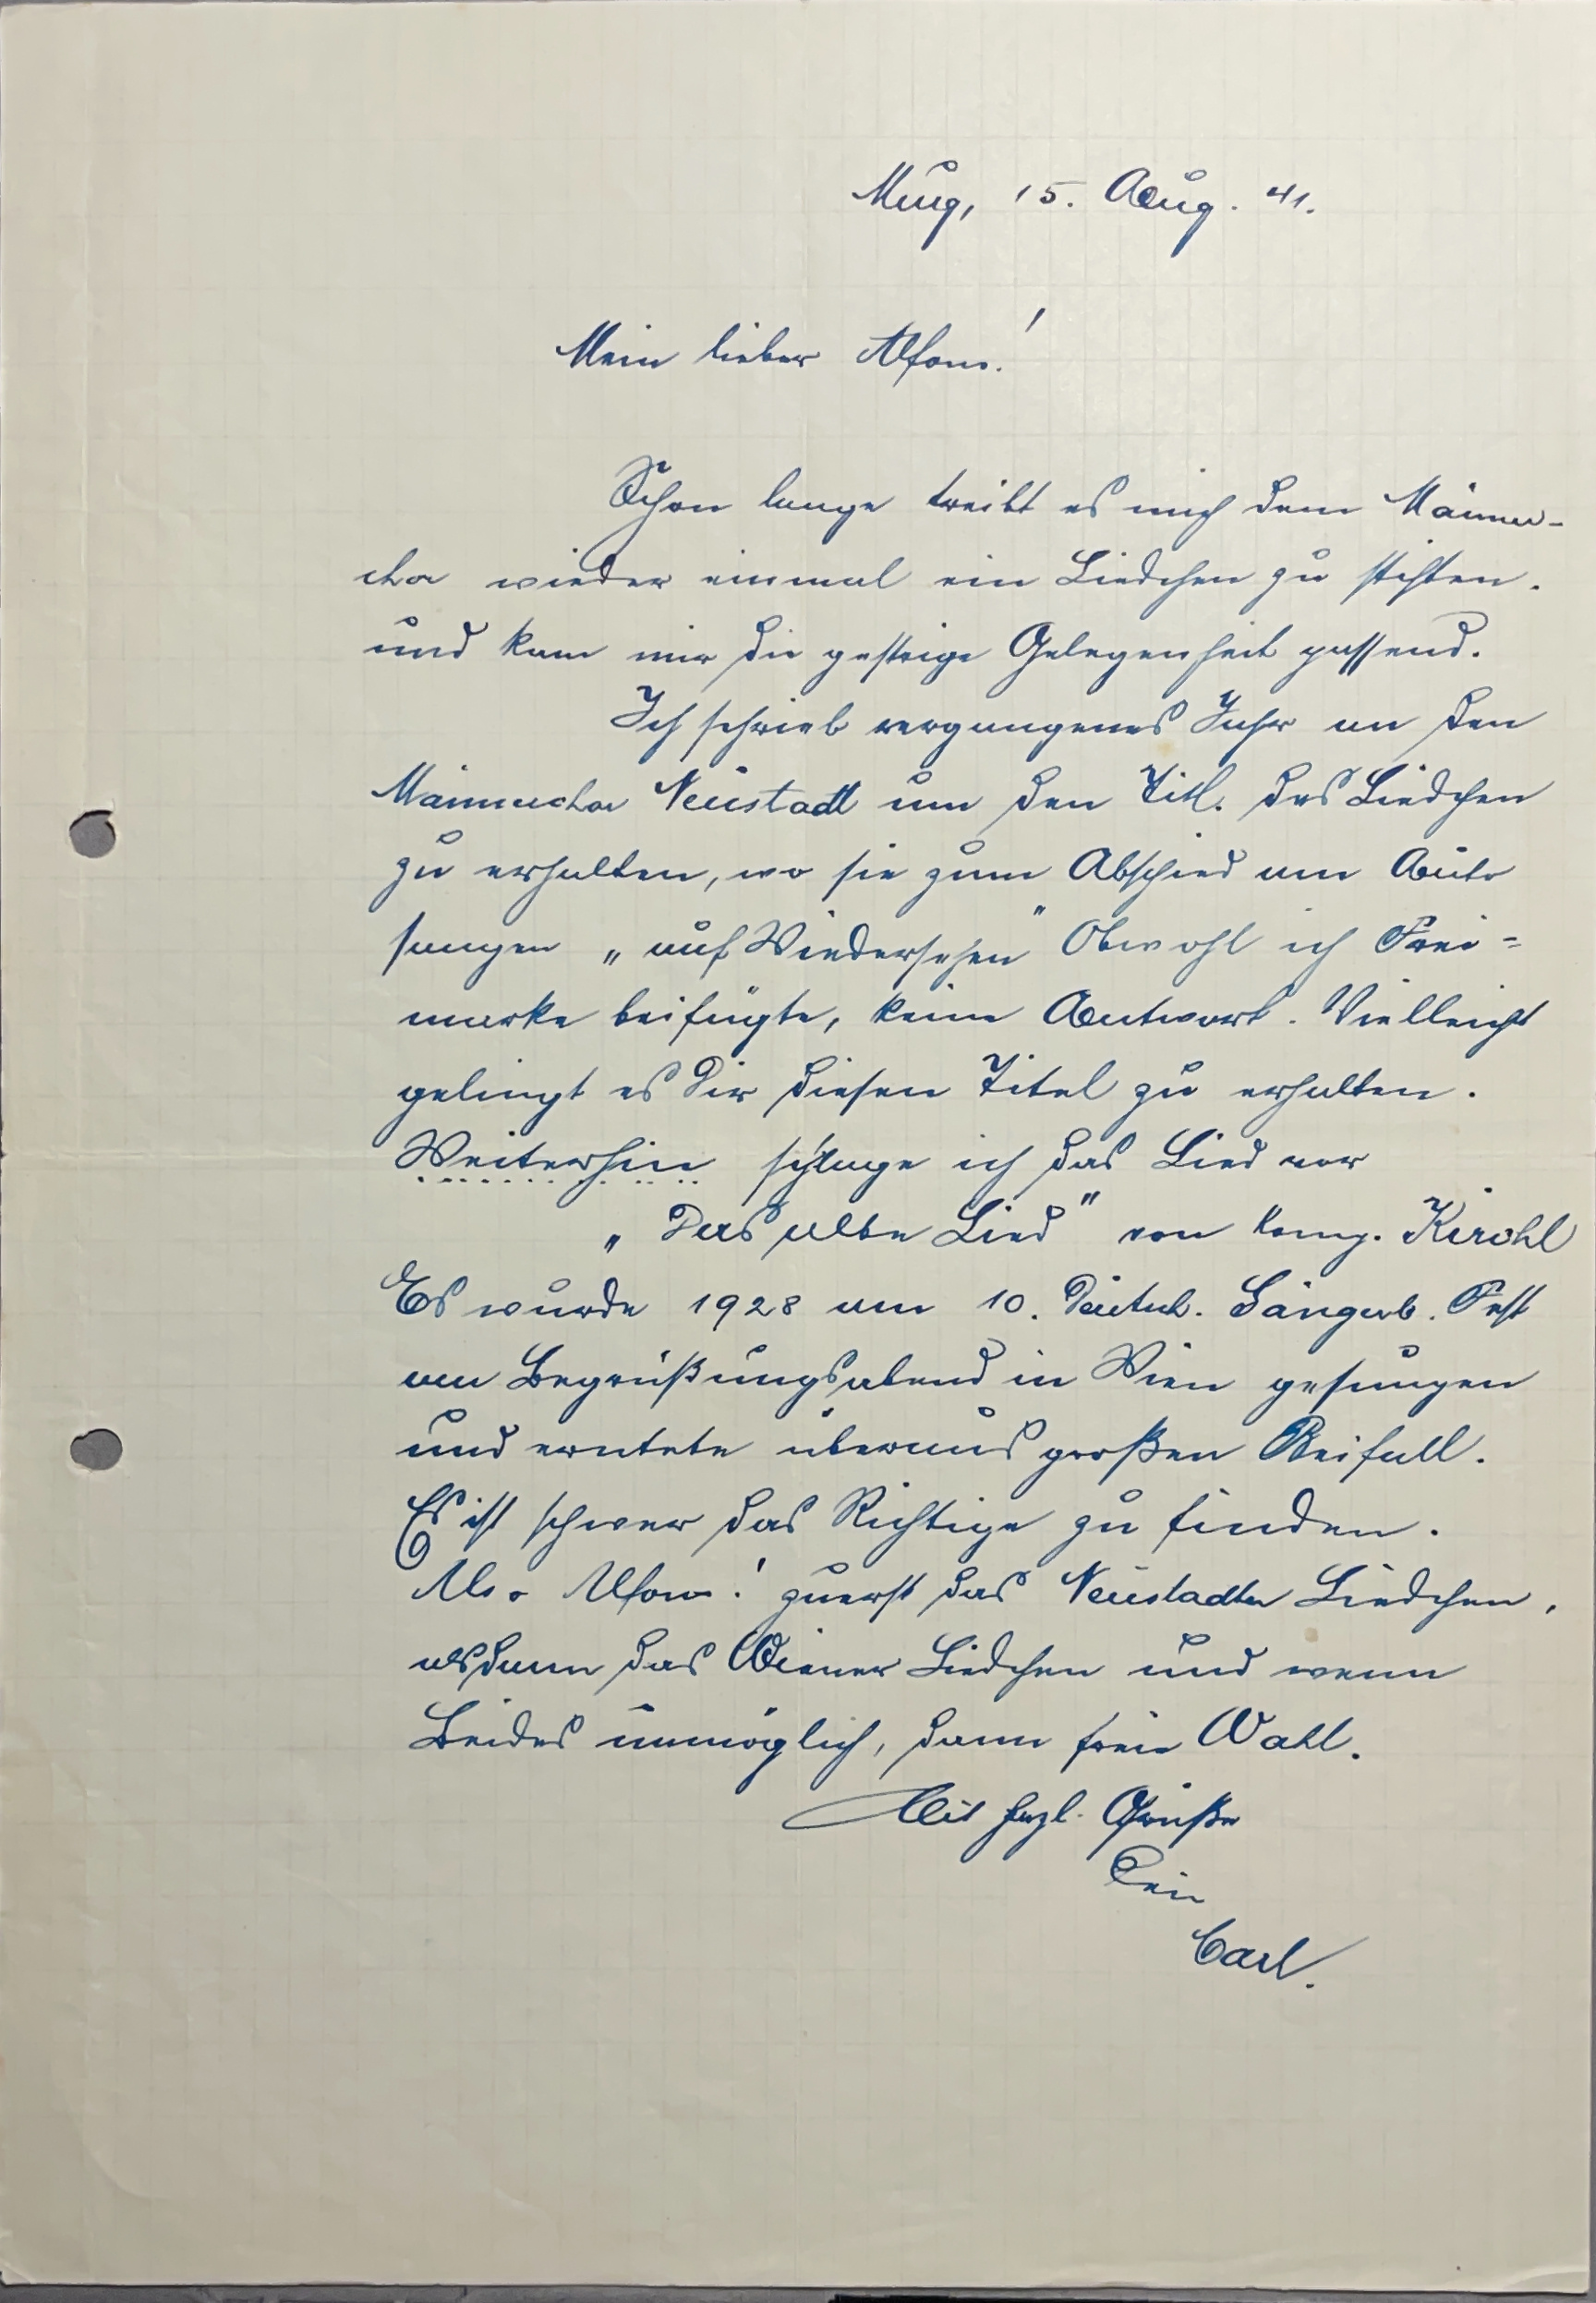
\includegraphics[width=\textwidth]{./assets/Images/Akte_076_S001.jpg}
  \caption{Beispiel für handschriftlichen Text in Akte\_076 erkannt mit Transkribus}\label{}
\end{figure}

  \begin{figure}[htbp]
  \centering
  \begin{tcolorbox}[colback=oldLetter, colframe=black, sharp corners, width=\textwidth]
    Murg. 15. Aug 41 

    
    Mein lieber Alfons! 

    Sehen lunge Lreitt es mich dem Männer- 

    chor wieder einmal ein Liedehen zu stehten. 

    und kam mir die gestege Gelegenheit gussend. 

    Männechor Venstad um den Title das Liedchen 

    zu erhalten, wo sie zum Abschied am Aute 

    sängen ``auf Wiederschen Owohl ich Frei! 

    märke beifügte, keine Aentwarb. Vielleicht 

    gelingt es Dir diesen Iitel zu erhalten. 
    
    Weiterhin sänge ich fal Lied nur 
    
    ``Bas alte Lied'' von being. Rerohl 

    Es wurde 1928 am 10. Dachub. Sängerb. Frst 

    von Begrüssungsabend in Dien gesungen. 

    und erntete überaus grossen Reifall. 

    Es ich schwer das Richtige zu finden. 

    Aler Alfon, werst das Vemsladler Liedchen. 

    alsdann das Biener Lidchen und wenn 

    Leides unmöglich, dann freu Nall. 

    Mit herzl. Grüsse 

    Dein 

    Carl 
  \end{tcolorbox}
  \caption{Transkription von \autoref{fig:Carl-handschrift}}
  \label{fig:Carl-Transkribus}

\end{figure}

ChatGPT produziert daraus:

\begin{tcolorbox}[colback=oldLetter, colframe=black, sharp corners, width=\textwidth]
Murg, 15. Aug. 41

Mein lieber Alfons!

Schon lange treibt es mich, dem Männerchor wieder einmal ein Liedchen zu stiften, und kam mir die günstige Gelegenheit gelegen.

Ich schrieb vergangenes Jahr an den Männerchor Venstad, um den Titel des Liedchens zu erhalten, das sie zum Abschied am Auto sangen: \enquote{Auf Wiedersehen, o wohl ich frei!}

Ich fügte eine Frankierung bei, erhielt jedoch keine Antwort. Vielleicht gelingt es Dir, diesen Titel zu erhalten.

Weiterhin sang ich das Lied nur \enquote{Das alte Lied von Wien}. Obwohl es am 10. Dezember 1928 beim Sängerbund-Fest von Begrüssungsabend in Wien gesungen wurde und überaus grossen Beifall erntete, ist es schwer, das Richtige zu finden.

Aber Alfons, zuerst das Venstadler Liedchen, dann das Wiener Liedchen und wenn beides unmöglich, dann Fröhlichsein.

Mit herzlichen Grüssen

Dein

Carl
\end{tcolorbox}
\captionof{figure}{Transkription durch ChatGPT von \autoref{fig:Carl-Transkribus}}
\label{fig:Carl-LLM}

Durch ChatGPT verliert der Text zwar seine ursprüngliche Formatierung und Zeilenumbrüche, aber wird nun nahezu fehlerfrei lesbar. Nur das \enquote{Venstadler Liedchen} ist eigendlich eines aus \enquote{Neustadt}. Eine anschliessende menschliche Korrektur ermöglicht also den Abgeleich mit dem nun lesbaren Text, und die Korrektur der Transkription.

Korrigiert und getagt lautet der Brief nun:
  \begin{figure}[htbp]
  \centering
\begin{tcolorbox}[colback=oldLetter, colframe=black, sharp corners, width=\textwidth]
  \textbf{\colorbox{place}{\texttt{Murg}}}.  \textbf{\colorbox{date}{\texttt{15. Aug 41}}} \\
\\
Mein lieber  \textbf{\colorbox{person}{\texttt{Alfons}}}!\\
Seit langem treibt es mich dem  \textbf{\colorbox{organization}{\texttt{Männer-}}}\\
\textbf{\colorbox{organization}{\texttt{chor}}} wieder einmal ein Liedchen zu stiften.\\
und kam mir die günstige Gelegenheit passend.\\
Ich schrieb vergangenes Jahr an den\\
Männechor Vorstand um den Titel das Liedchen\\
zu erhalten, wo sie zum Abschied am Auto \\
sangen \enquote{auf Wiederschen} Obwohl ich  \textbf{\colorbox{unclear}{\texttt{Frank-}}}\\
marke beifügte, keine Antwort. Vielleicht\\
gelingt es Dir diesen Titel zu erhalten.\\
Weiterhin sänge ich das Lied nur\\
\enquote{Das alte Lied} von  \textbf{\colorbox{abbrev}{\texttt{Komp.}}}\textbf{\colorbox{person}{\texttt{ Kirchl}}}\\
Es wurde \textbf{\colorbox{date}{\texttt{1928}}} am \textbf{\colorbox{eventTag}{\texttt{10. Deutsch. Sängerb. Fest}}}\\
am Begrüssungsabend in \textbf{\colorbox{place}{\texttt{Wien}}} gesungen.\\
und erntete überaus grossen Beifall.\\
Es ich schwer das Richtige zu finden.\\
Also \textbf{\colorbox{person}{\texttt{Alfons}}}! zuerst das \textbf{\colorbox{place}{\texttt{Neustadter}}} Liedchen.\\
alsdann das \textbf{\colorbox{place}{\texttt{Wiener}}} Liedchen und wenn\\
Beides unmöglich, dann freie Wahl.\\
Mit herzl. Grüssen \\
Dein\\
\textbf{\colorbox{person}{\texttt{Carl}}}\\
\end{tcolorbox}
\caption{Tagging von \autoref{fig:Carl-LLM}}\label{fig:Tagging-Carl-LLM}
\end{figure}
\begingroup
\begin{figure}[htbp]
\begin{tcolorbox}[colback=oldLetter, colframe=black, sharp corners, width=\textwidth]
\textbf{\colorbox{place}{\texttt{München}}}, \textbf{\colorbox{date}{\texttt{28.V.1941}}} \\
\\
Lieber \textbf{\colorbox{person}{\texttt{Otto}}}!\\
Nur wer die Sehnsucht kennt weiss was ich leide\\
Ich wandle traurig her in schwarzer Seide.\\
Die Sehnsucht brennt, du bist so fern.\\
Ach lieber \textbf{\colorbox{person}{\texttt{Otto}}}, wie hab ich dich gern.\\
Ich schnitt es gern in alle Rinden.\\
Ach \textbf{\colorbox{person}{\texttt{Otto}}}, wann u.\ \ wo kann ich dich finden?\\
Deine dich nie vergessende\\
\textbf{\colorbox{person}{\texttt{Lina Fingerdick}}}\\
\\
An\\
\textbf{\colorbox{person}{\texttt{Herrn Otto Bollinger}}}\\
z.Hd. \textbf{\colorbox{person}{\texttt{Herrn Alfons Zimmermann}}}\\
\textbf{\colorbox{organization}{\texttt{Vereinsführer des Männerchor}}}\\
\textbf{\colorbox{place}{\texttt{Murg}}}\\
\textbf{\colorbox{place}{\texttt{Laufenburg (Baden)}}}\\
\textbf{\colorbox{place}{\texttt{Rhina}}}
\end{tcolorbox}
\end{figure}
\endgroup

%––––––––––––––––––––––––––––––––––––––––––––––––––––––––––––––––––––––––––––––––––––––%
%––––––––––––––––––––––––––––––––––––––––––––––––––––––––––––––––––––––––––––––––––––––%
%––––––––––––––––––––––––           Bibliographie         –––––––––––––––––––––––––––––%
%––––––––––––––––––––––––––––––––––––––––––––––––––––––––––––––––––––––––––––––––––––––%
%––––––––––––––––––––––––––––––––––––––––––––––––––––––––––––––––––––––––––––––––––––––%
\pagecolor{white}
\newpage
\begingroup
\small
\singlespacing%
\printbibliography[
heading=bibintoc,
title={Bibliographie}%title of the 'references' section, change this if necessary
]%
\endgroup

\newpage
\appendix
\section{Anhang}
\begingroup
\small
\subsection{PDF\_to\_JPEG.py}\label{section:PDF_to_JPEG}
\begin{minted}[
frame=lines,
framesep=2mm,
baselinestretch=1.2,
bgcolor=LightGray,
fontsize=\footnotesize,
linenos,
breaklines=true,  %Automatischer Zeilenumbruch
breakanywhere=true % Minted darf überall umbrechen (optional)
]{python}
import os
import fitz  # PyMuPDF

def convert_pdf_to_jpg(src_folder, dest_folder):
    # Überprüfen, ob der Zielordner existiert, und ihn ggf. erstellen
    if not os.path.exists(dest_folder):
        os.makedirs(dest_folder)

    # Durchgehen durch alle Dateien im Quellordner
    for root, dirs, files in os.walk(src_folder):
        for file in files:
            # Überprüfen, ob die Datei eine PDF-Datei ist
            if file.lower().endswith(".pdf"):
                # Vollständigen Pfad zur PDF-Datei erstellen
                pdf_path = os.path.join(root, file)
                # PDF-Datei öffnen
                doc = fitz.open(pdf_path)
                # Durch alle Seiten der PDF-Datei gehen
                for page_num in range(len(doc)):
                    page = doc[page_num]
                    # Seite in ein PixMap-Objekt umwandeln (für die Konvertierung in JPG)
                    pix = page.get_pixmap()
                    # Dateinamen ohne Dateiendung extrahieren
                    filename_without_extension = os.path.splitext(file)[0]
                    # Ausgabedateinamen erstellen mit führenden Nullen für die 
                    # Seitennummer
                    output_filename = f"{filename_without_extension}_S{page_num + 1:03d}.jpg"


                    # Vollständigen Pfad zur Ausgabedatei erstellen
                    output_path = os.path.join(dest_folder, output_filename)
                    # Bild speichern
                    pix.save(output_path)
                # PDF-Datei schliessen
                doc.close()
                
                # Erfolgsmeldung ausgeben
                print(f"{file} wurde erfolgreich umgewandelt und gespeichert
                in {dest_folder}")

# Pfade zu den Ordnern mit den PDF-Dateien (Quelle) und den JPG-Dateien (Ziel)
src_folder = r"/Users/svenburkhardt/Documents/D_Murger_Männer_Chor_Forschung/Scan_Männerchor/Männerchor_Akten_1925–1945/Scan_Männerchor_PDF"
dest_folder = r"/Users/svenburkhardt/Documents/D_Murger_Männer_Chor_Forschung/Masterarbeit/JPEG_Akten_Scans"


# Funktion aufrufen, um die Konvertierung durchzuführen
convert_pdf_to_jpg(src_folder, dest_folder)

\end{minted}
\subsection{Tagging in Transkribus}


    Transkribus und seine Modelle unterstützen nicht nur beim Transkribieren der Texte, sondern erlauben auch das Taggen von \textit{Named Entities}.  
    Für die vorliegende Arbeit sind dabei besonders Personen, Orte, Organisationen und Daten relevant.  
    Um hierfür ein stringentes Verfahren zu entwickeln, wurden die Tags wie folgt definiert:
    
    \begin{description}

    % Abbreviations
    \item \textbf{\colorbox{abbrev}{\texttt{abbrev}}}
        
    Mit dem Tag \texttt{\texttt{\textbf{{\colorbox{abbrev}{abbrev}}}}} werden alle Abkürzungen getaggt, die für eine eindeutige Entität stehen. 
    
    \noindent\textbf{\ding{43} Beispiel 1}: Dr., Prof., St., Hr., Frl., Dipl.-Ing., etc.
    
    \textbf{\ding{43} Beispiel 2}: Organisationskürzel, wenn sie eindeutig sind: 
    \colorbox{VeryLightGray}{\textless\ \  abbrev\textgreater\ \  V.D.A.\textless\ \  /abbrev\textgreater}.

    \textbf{\textbf{\ding{43} Beispiel 3}}: Falls eine dazugehörige Entität vorhanden ist, wird die Abkürzung getaggt und wird gleichzeitig als zugehörige Entität getaggt:
    
    \colorbox{VeryLightGray}{\textless\ \  person\textgreater\ \  \textless\ \  abbrev\textgreater\ \  Dr.\textless\ \  /abbrev\textgreater\ \  Weiss{\textless\ \  /person\textgreater}}

    
    % Unclear    
    \item \textbf{\colorbox{unclear}{\texttt{unclear}}}
    

    Mit dem Tag \texttt{\texttt{\textbf{{\colorbox{unclear}{unclear}}}}} werden unleserliche oder schwer entzifferbare Textstellen markiert. 

    
    \noindent\textbf{\ding{43} Beispiel 1}: Unklare Zeichen oder fehlende Buchstaben: 

    \colorbox{VeryLightGray}{\enquote{Er wohnte in\textless\ \  unclear\textgreater\ \  [\ldots]\textless\ \  unclear\textgreater}.}

    \textbf{\ding{43} Beispiel 2}: Teilweise lesbare Wörter:

    \colorbox{VeryLightGray}{\enquote{{\textless\ \  place\textgreater\ \  Frei\textless\ \  unclear\textgreater\ \  [\ldots]\textless\ \  unclear\textgreater\ \  \textless\ \  place\textgreater}}.}
    
%Sic   
    \item\texttt{\textbf{{\colorbox{sic}{sic}}}} 

    Mit dem Tag \texttt{sic} werden Wörter markiert, die im Originaltext in einer falschen oder ungewöhnlichen Schreibweise geschrieben wurden. 
    
    \noindent\ding{43} Beispiel 1: Veraltete oder falsche Schreibweisen: 

    \colorbox{VeryLightGray}{\enquote für dass.}

    \ding{43} Beispiel 2: Offensichtliche Tippfehler, wenn sie im Originaltext so vorkommen: 

    \colorbox{VeryLightGray}{\enquote{Wir haben {<sic>einen</sic>} grosse Freude.}}

    \ding{43} Beispiel 3: Falls eine Korrektur notwendig ist, kann sie als Kommentar ergänzt werden. 

    \end{description}

    \subsubsection{Inhaltliche Tags}
    \begin{description}
    % Person
    \item\texttt{\textbf{{\colorbox{person}{person}}}}
        
    Mit dem Tag \texttt{\colorbox{person}{person}} sollen alle Strings getaggt, die eine direkte Zuordnung einer Person ermöglichen.
    
    \noindent \textbf{\ding{43} Beispiel 1}: Vereinsführer, Alfons, Zimmermann, Alfons Zimmermann, Z. A. Zimmermann, Herr Zimmermann, Herr Alfons Zimmermann, etc. 

    \textbf{\ding{43} Beispiel 2}: Funktionen wie Oberlehrer, Chorleiter, etc.
    Wenn Ort, Name oder Organisation bekannt sind. Eine Person kann sowohl mit ihrem Namen als auch ihrer Funktion (wie Dirigent) getaggt werden.  
    Aus der Korrespondenz ist in der Regel eine zugehörige Organisation ersichtlich, mit deren Verknüpfung eine namentlich nicht genannte Person identifiziert werden könnte.

    
    % Signature    
    \item\texttt{\textbf{{\colorbox{signature}{signature}}}}
        
    Mit dem Tag \texttt{\colorbox{signature}{signature}} werden alle Strings getaggt, die eine handschriftliche Unterschrift darstellen.  
    Der Tag \texttt{\colorbox{signature}{signature}} ist nahezu deckungsgleich mit dem Tag \texttt{\colorbox{person}{person}}.  
    Er dient zur \textbf{graduellen Unterscheidung}, ob ein Name im Fliesstext als gesichert leserlich oder handschriftlich als Signatur vorliegt.  
    
    \noindent \textbf{\ding{43} Beispiel 1}: Eindeutig lesbare Signaturen werden direkt getaggt:  

    \colorbox{VeryLightGray}{\texttt{\textless\ \  signature\textgreater\ \  A. Zimmermann\textless\ \  /signature\textgreater}}. 

    \textbf{\ding{43} Beispiel 2}: Teilweise unleserliche Signaturen werden mit dem Tag \texttt{\colorbox{unclear}{unclear}} innerhalb von \texttt{\colorbox{signature}{signature}} markiert: 

    \colorbox{VeryLightGray}{\texttt{\textless\ \  signature\textgreater\ \  R. We\textless\ \  unclear\textgreater\ \  [\ldots]\textless\ \  /unclear\textgreater\textless\ \  /signature\textgreater}}. 

    
    \textbf{\ding{43} Beispiel 3}: Wenn nur ein Teil des Namens lesbar ist, aber eine Identifikation unsicher bleibt, sollte die Unterschrift 
    vollständig im Tag \texttt{\colorbox{unclear}{unclear}} innerhalb von \texttt{\colorbox{signature}{signature}} stehen:\\

    \colorbox{VeryLightGray}
    {\texttt{\textless\ \  signature\textgreater\ \  \textless\ \  unclear\textgreater\ \  \textit{etwas unleserliches}\textless\ \  /unclear\textgreater\ \  \textless\ \  /signature\textgreater}.} 
    
    \textbf{\ding{43} Beispiel 4}: Wenn eine Signatur einer bekannten Person zugeordnet werden kann, aber nicht vollständig lesbar ist, bleibt die Signatur erhalten und wird \textbf{ohne} den Tag \texttt{\colorbox{person}{person}} zu verwenden: 

    \colorbox{VeryLightGray}{\texttt{\textless\ \  signature\textgreater\ \  A. Zimm\textless\ \  unclear\textgreater\ \  [\ldots]\textless\ \  /unclear\textgreater\textless\ \  /signature\textgreater}.} 
    
    \textbf{\ding{43} Beispiel 5}: Wenn eine Unterschrift vollständig transkribiert wurde und die Person bekannt ist, wird sie nur mit \texttt{\colorbox{signature}{signature}} getaggt, \textbf{ohne} den Tag \texttt{\colorbox{person}{person}} zu verwenden:  

    \colorbox{VeryLightGray}{\texttt{\textless\ \  signature\textgreater\ \  Alfons Zimmermann\textless\ \  /signature\textgreater}.} 
    
    % Organization    
    \item\texttt{\textbf{{\colorbox{organization}{organization}}}}
        
    Mit dem Tag \texttt{\colorbox{organization}{organization}} werden alle Strings getaggt, die eine direkte Zuordnung einer Organisation ermöglichen.  
    
    \noindent \textbf{\ding{43} Beispiel 1}: Männerchor Murg, Verein Deutscher Arbeiter (V.D.A.), Murgtalschule, etc.

    \textbf{\ding{43} Beispiel 2}: Abkürzungen, wenn sie eine Organisation eindeutig bezeichnen, z.B. V.D.A., NSDAP, STAGMA, etc.
    

    % Place    
    \item\texttt{\textbf{{\colorbox{place}{place}}}}
        
    Mit dem Tag \texttt{\colorbox{place}{place}} werden alle Strings getaggt, die sich auf einen geografischen Ort beziehen.  
    
    \noindent \textbf{\ding{43} Beispiel 1}: Murg (Baden), Freiburg, Berlin, Murgtal, Schwarzwald, etc.

    \textbf{\ding{43} Beispiel 2}: Orte mit näherer Bestimmung, z.B. \enquote{bei Berlin}, \enquote{im Murgtal} werden getaggt:  

    \colorbox{VeryLightGray}{\texttt{\textless\ \  place\textgreater\ \  im Murgtal\textless\ \  /place\textgreater}.} 

    
    % Date    
    \item\texttt{\textbf{{\colorbox{date}{date}}}}
        
    Mit dem Tag \texttt{\colorbox{date}{date}} werden alle expliziten und implizierten Datumsangaben markiert.  
    
    \noindent \textbf{\ding{43} Beispiel 1}:  29.05.1936

    \textbf{\ding{43} Beispiel 2}: 29. Mai 1936

    \textbf{\ding{43} Beispiel 3}: den 29.\ \  d. Mts.:

    \colorbox{VeryLightGray}{\texttt{\textless\ \  date when=\enquote{29.05.1936}\textgreater\ \  den 2.\textless\ \  /date\textgreater} \texttt{\textless\ \  abbrev\textgreater\ \  d. Mts.\textless\ \  /abbrev\textgreater}}

% Event
    \item\texttt{\textbf{{\colorbox{eventTag}{event}}}}
    
    Mit dem Tag \texttt{\colorbox{eventTag}{event}} werden expliziten und implizierten Ereignisse markiert. Diese Ereignisse haben einen zeitlichen oder räumlichen Bezug, und können benannt werden. Dazu zählen:

    \noindent \textbf{\ding{43} Beispiel 1}: \enquote{Jubiläumskonzert}

    \textbf{\ding{43} Beispiel 2} \enquote{Gründung des Vereins} 

    \textbf{\ding{43} Beispiel 2}\enquote{Kriegsausbruch} oder \enquote{Kriegsende}

    Konzepte, die nicht klar in den Texten benannt werden, wie beispielsweise die Suche nach einem Dirigenten, können nicht immer Ereignis getaggt werden. Sie sollen später aber in der Datenbank implementiert werden.
    \end{description}
    
    \subsubsection{Strukturelle Tags}
    \begin{description}

    % Abbreviations
    \item\texttt{\textbf{{\colorbox{abbrev}{abbrev}}}}
    
        
    Mit dem Tag \texttt{\texttt{\textbf{{\colorbox{abbrev}{abbrev}}}}} werden alle Abkürzungen getaggt, die für eine eindeutige Entität stehen.

    
    \noindent\textbf{\ding{43} Beispiel 1}: Dr., Prof., St., Hr., Frl., Dipl.-Ing., etc.

    \textbf{\ding{43} Beispiel 2}: Organisationskürzel, wenn sie eindeutig sind:\\\colorbox{VeryLightGray}{\textless\ \  abbrev\textgreater\ \  V.D.A.\textless\ \  /abbrev\textgreater}.

    \textbf{\textbf{\ding{43} Beispiel 3}}: Falls eine dazugehörige Entität vorhanden ist, wird die Abkürzung getaggt und wird gleichzeitig als zugehörige Entität getaggt:

    \colorbox{VeryLightGray}{\textless\ \ person\textgreater\ \  \textless\ \  abbrev\textgreater\ \  Dr.\textless\ \  /abbrev\textgreater\ \  Weiss{\textless\ \  /person\textgreater}}
    
    % Unclear    
    \item\texttt{\textbf{{\colorbox{unclear}{unclear}}}}
    

    Mit dem Tag \texttt{\texttt{\textbf{{\colorbox{unclear}{unclear}}}}} werden unleserliche oder schwer entzifferbare Textstellen markiert.
    
    \noindent\textbf{\ding{43} Beispiel 1}: Unklare Zeichen oder fehlende Buchstaben: 

    \colorbox{VeryLightGray}{\enquote{Er wohnte in\textless\ \ unclear\textgreater\ \ [\ldots]\textless\ \ unclear\textgreater}.}

    \textbf{\ding{43} Beispiel 2}: Teilweise lesbare Wörter:

    \colorbox{VeryLightGray}{\enquote{{\textless~place\textgreater~Frei\textless~unclear\textgreater~[\ldots]\textless~unclear\textgreater~\textless~place\textgreater}}.}

    
%Sic   
    \item\texttt{\textbf{{\colorbox{sic}{sic}}}} 

    Mit dem Tag \texttt{sic} werden Wörter markiert, die im Originaltext in einer falschen oder ungewöhnlichen Schreibweise geschrieben wurden.

    \noindent\ding{43} Beispiel 1: Veraltete oder falsche Schreibweisen: 

    \colorbox{VeryLightGray}{\enquote für dass.}

    \ding{43} Beispiel 2: Offensichtliche Tippfehler, wenn sie im Originaltext so vorkommen: 

    \colorbox{VeryLightGray}{\enquote{Wir haben {<sic>einen</sic>} grosse Freude.}}

    \ding{43} Beispiel 3: Falls eine Korrektur notwendig ist, kann sie als Kommentar ergänzt werden. 

    \end{description}
    \endgroup
\end{document}
